\documentclass[10pt,twoside,a4paper]{memoir}
\usepackage[ascii]{}
\usepackage[french]{babel}
\usepackage[T1]{fontenc}
\usepackage{longtable}
\usepackage[utf8]{inputenc}
\usepackage{lmodern}
\usepackage{lettrine}
\usepackage{geometry}
\usepackage{amsmath,amssymb,amsfonts,amsgen,amsbsy,textcomp,pifont}
\usepackage{bbold,stackrel,dsfont,mathrsfs,soul,tcolorbox,verbatimbox}
\usepackage{amsthm}
\usepackage{textcomp}
\usepackage{color}
\usepackage{xcolor}
\usepackage{colortbl}
\usepackage{ae,aecompl}
\usepackage{graphicx}
\DeclareGraphicsExtensions{.pdf}
\usepackage{fancyhdr}
\usepackage{fancybox}
\usepackage{fancyvrb}
\usepackage[open=true]{bookmark}
\usepackage{caption}
\usepackage{subcaption}
\usepackage{listings}
\usepackage{array,multirow,multicol}
\usepackage{lastpage}
\usepackage{cellspace}
\usepackage{enumitem}
\usepackage{float}
\usepackage{xspace}
\usepackage{layout}
\usepackage{epsfig}
\usepackage{epstopdf}
\usepackage{pifont}
\usepackage{ulem}
\usepackage{url}
\usepackage{rotating}
\usepackage{chngcntr}
%%%%%   ALE   %%%%%
\usepackage{microtype}
\usepackage{tabularx}
\usepackage{stmaryrd}
\usepackage{cleveref}
\usepackage{empheq,etoolbox}
\usepackage{tikz}
\usetikzlibrary{arrows}
\newcommand\irregularcircle[2]{% radius, irregularity
  \pgfextra {\pgfmathsetmacro\len{(#1)+rand*(#2)}}
  +(0:\len pt)
  \foreach \a in {10,20,...,350}{
    \pgfextra {\pgfmathsetmacro\len{(#1)+rand*(#2)}}
    -- +(\a:\len pt)
  } -- cycle
}
\def\b_v{\mathbf{v}}
\def\U{\mathbf{U}}
\def\V{\mathbf{V}}
\renewcommand{\div}{\mathrm{div}}
\newcommand{\velocity}{\vec{u}}
\newcommand{\vale}{\vec{u}_{\text{ALE}}} 
\newcommand{\normal}{\vec{ n}}
\newcommand{\point}{x}

%%%%%   CMFD   %%%%%

\DeclareMathAlphabet{\mathpzc}{OT1}{pzc}{m}{it}
\def\l|{\left|\left|}
\def\r|{\right|\right|}
\def\R{\mathds R}
\def\P{\mathds P}
\def\N{\mathds N}
\def\Z{\mathds Z}
\def\E{\mathds E}
\def\1{\mathds 1}
\def\T{{\sf T}}
\def\B{{\sf B}}
\def\S{{\sf S}}
\def\G{{\sf G}}
\def\Vect{\mathrm{ Vect}}
\def\th{\mathrm{\,th\,}}
\def\ch{\mathrm{\,ch\, }}
\def\argth{\mathrm{\,ath\, }}
\def\sh{\mathrm{\,sh\, }}
\def\ve{\varepsilon}
\def\hZ{\hat Z}
\def\hpsi{\hat \psi}
\def\cM{{\cal M}}
\def\de{{\rm d}}
\def\red{\color{red}}
\def\pink{\color{pink}}
\def\blue{\color{blue}}
\def\green{\color{green}}
\def\gray{\color{gray}}
\def\white{\color{white}}

%%%%%   SENSITIVITY   %%%%%
\def\b_u{\mathbf{u}}

%%%%%   Phase_field   %%%%%
\usetikzlibrary{trees}
\usetikzlibrary{decorations.pathmorphing}
\usetikzlibrary{decorations.markings}
\usetikzlibrary{arrows,shapes,patterns}
\usetikzlibrary{fpu}
\usepackage{pdflscape}
\usepackage{footmisc}
\usepackage[mathscr]{eucal}
\usepackage{framed,verbatim,alltt}

\newenvironment{disarray}%
 {\everymath{\displaystyle\everymath{}}\array}%
 {\endarray}

\lstset{upquote=true,
        columns=fullflexible,
        keepspaces=true,
        breaklines,
        breakindent=0pt,
        basicstyle=\ttfamily\small
        }
% \definecolor{blizzardblue}{rgb}{0.67, 0.9, 0.93}
\makeatletter
\newsavebox{\lstb@x}
\lstnewenvironment{inputfile}
  {\setbox\lstb@x\hbox\bgroup\color@setgroup}
  {\color@endgroup\egroup\colorbox{gray!25}{\usebox{\lstb@x}}}
\makeatother

% \definecolor{blizzardblue}{rgb}{0.67, 0.9, 0.93}
%\lstnewenvironment{inputfile}
%{\lstset{backgroundcolor=\color{blizzardblue},mathescape=true,basicstyle=\ttfamily, columns=fullflexible, keepspaces=true}}{}
 
%%%%%%%%%%%%%%%%%%%%%%%%%%%%%%%%%%%%%%%%%%%%%%%%%%%%%%%%%%%%%
% espacement table des matieres et des figures entre numero et titre
\usepackage{tocloft}
\newcommand{\DF}{\displaystyle\frac}
\renewcommand{\cftpartnumwidth}{3em}
\cftsetindents{figure}{0em}{4em}
\cftsetindents{table}{0em}{4em}
%
% Pour supprimer les encadres rouges des liens et definir leur fonte en bleu
\usepackage{imakeidx}
\usepackage{hyperref}
\hypersetup{linkcolor=blue,colorlinks=true,bookmarks=true,bookmarksopen=true,bookmarksnumbered=true}
%
\setlength\hoffset{0cm}
\setlength\voffset{0cm}
\setlength\oddsidemargin{0cm}
\setlength\evensidemargin{0cm}
\setlength\topmargin{0cm}
\setlength\headheight{0.45cm}
\setlength\headsep{0.6cm}
\setlength\marginparsep{0cm}
\setlength\marginparwidth{0cm}
\setlength\footskip{1.4cm}
\setlength{\textheight}{670pt} 
\setlength\textwidth{16.4cm}
\setlength{\cellspacebottomlimit}{5pt}
\setlength{\cellspacetoplimit}{5pt}
\setlength{\parindent}{0pt}
\setcounter{tocdepth}{2}
\setsecnumdepth{section}
% espacement corps de texte
\baselineskip=14pt
%
% redefinition de la numerotation des figures et des tableaux
\renewcommand{\thefigure}{\Roman{part}.\arabic{chapter}.\arabic{figure}}
\renewcommand{\thetable}{\Roman{part}.\arabic{chapter}.\arabic{table}}
%
\makeatletter
%% Because html converters don't know tabularnewline
\floatstyle{ruled}\providecommand{\tabularnewline}{\\}
%% nouvelle commande algorithm pour des zones de code
\floatstyle{ruled}
\newfloat{algorithm}{tbp}{loa}[chapter]
\providecommand{\algorithmname}{Algorithm}
\floatname{algorithm}{\protect\algorithmname}
%
\makeatother
%
\fancypagestyle{part}{%
%%\fancyhead[L]{}
%%\fancyhead[R]{\textit{\rightmark}}
\lfoot{\textit{TrioCFD Models Documentation}}
\cfoot{}
\rfoot{\thepage}
\renewcommand{\headrulewidth}{0.5pt}
\renewcommand{\footrulewidth}{0.3pt}}
%
\fancypagestyle{chapter}{%
%%\fancyhead[L]{\textit{\rightmark}}
%%\fancyhead[R]{}
\lfoot{\textit{TrioCFD Models Documentation}}
\cfoot{}
\rfoot{\thepage}
\renewcommand{\headrulewidth}{0.5pt}
\renewcommand{\footrulewidth}{0.3pt}}
%
\pagestyle{fancy}
\renewcommand{\chaptermark}[1]{\markboth{#1}{#1}}
\renewcommand{\sectionmark}[1]{\markright{#1}}
\renewcommand{\headrulewidth}{0.5pt}
\renewcommand{\footrulewidth}{0.3pt}
%numerotation equation
\renewcommand{\theequation}{\thepart.\thesection~~eq\arabic{equation}}
%%\lhead{\leftmark}
\chead{}
%%\rhead{\rightmark}
\lfoot{\textit{TrioCFD Models Documentation}}
\cfoot{}
\rfoot{\thepage}
%
% definition du style des parties
\usepackage{indentfirst}
\renewcommand{\beforepartskip}{\null\vskip 5pt plus 1.8fil \newpage}
\renewcommand{\afterpartskip}{\vskip 0pt plus 0.0fil }
\renewcommand*{\partnumfont}{\normalfont\HUGE\sffamily}
\renewcommand*{\parttitlefont}{\normalfont\Huge\sffamily}
\renewcommand{\part}[1]{%
  \phantomsection
  \refstepcounter{part}%
  \addcontentsline{toc}{part}%
    {\protect\partnumberline{\thepart}#1}
  \pagestyle{part}
  \beforepartskip
  \begin{adjustwidth}{}{10mm}\printpartnum. \space \printparttitle{#1}\end{adjustwidth}
  \afterpartskip
  }
% definition du style des chapitres
%
\renewcommand{\clearforchapter}{\null\vskip 1pt}

\makechapterstyle{customchapstyle}{%
  \pagestyle{chapter}
  \clearforchapter
  \renewcommand*{\chapnumfont}{\normalfont\HUGE\sffamily}
  \renewcommand*{\chaptitlefont}{\normalfont\huge\sffamily}
  \settowidth{\chapindent}{\chapnumfont 111}
  \renewcommand*{\chapterheadstart}{\begingroup
    \vspace*{\beforechapskip}%
    \begin{adjustwidth}{}{}%
    \hrulefill
    \smash{\rule{0.4pt}{15mm}}
    \end{adjustwidth}\endgroup}
  \renewcommand*{\printchaptername}{}
  \renewcommand*{\chapternamenum}{}
  \renewcommand*{\printchapternum}{%
    \begin{adjustwidth}{}{}
    \hfill
    \raisebox{10mm}[0pt][0pt]{\chapnumfont \Roman{part}.\thechapter}%
                              \hspace*{1em}
    \end{adjustwidth}\vspace*{-3.0\onelineskip}}
  \renewcommand*{\printchaptertitle}[1]{%
    \vskip\onelineskip
    \raggedleft {\chaptitlefont ##1}\par\nobreak}}
%
\counterwithin*{chapter}{part}
%
\makeindex
%%%%%%%%%%%%%%%%%%%%%%%%%%%%%%%%%%%%%%%%%%%%%%%%%%%%%%%%%%%%%%%%%%%%%%%%%%%%%%%%%%%%%%
% debut du document
%%%%%%%%%%%%%%%%%%%%%%%%%%%%%%%%%%%%%%%%%%%%%%%%%%%%%%%%%%%%%%%%%%%%%%%%%%%%%%%%%%%%%%
\begin{document}
%
% 1ere page
\thispagestyle{empty}
%\cfoot{}
%\renewcommand{\headrulewidth}{0pt}
%\renewcommand{\footrulewidth}{0pt}
\begin{multicols}{2}
%%
\includegraphics[scale=0.75]{../pictures/cealogo.png}
\begin{flushright}\Ovalbox{\begin{minipage}{8cm} \begin{center} \vspace{0.4cm}\Large{DES/ISAS/DM2S/STMF/LMSF}\vspace{0.4cm}\end{center}\end{minipage}}\end{flushright}
\begin{flushright}\Ovalbox{\begin{minipage}{4cm} \begin{center} \vspace{0.4cm}\Large{\thepage/\pageref{LastPage}}\vspace{0.4cm}\end{center}\end{minipage}}\end{flushright}
\end{multicols}
\cornersize{.2}
\Ovalbox{\begin{minipage}{16.2cm}
\begin{center} \vspace{2cm}
\parbox[t]{12cm}{\hspace{1cm}\huge{\textbf{USER DOCUMENTATION :}}
\newline
\hspace{3cm}\LARGE{\textbf{Models Documentation TrioCFD}}} \end{center}
\vspace{0.4cm}
\begin{center}
\includegraphics[scale=0.5]{../pictures/TrioCFD.png} \end{center}
\vspace{0.4cm}
\begin{center}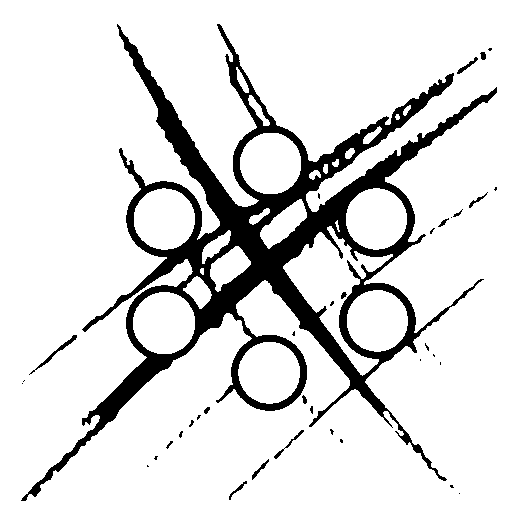
\includegraphics[scale=0.35]{../pictures/logo_DM2S.png} \end{center}
\vspace{0.4cm}
\setlength{\tabcolsep}{0.5cm}
\begin{tabular}{ Sc|Sc|Sc|Sc }
\hline
Code Version & Date & Code manager & Authors \\
 & & J. DARONA & \\ \hline
 & &\multirow{3}{*}{
\includegraphics[scale=0.6]{../validation_report/tools/sign_JD.png}} &  \\
v1.9.1 & \today && TrioCFD Team\\
 & &&  \\ \hline
\multicolumn{2}{Sc|}{ } & \multicolumn{2}{Sl}{\textit{Input file : } models\_report\_TrioCFD.tex } \\
\multicolumn{2}{c|}{\textbf{DES/ISAS/DM2S} } & \multicolumn{2}{l}{\textit{Software : } TrioCFD } \\
\multicolumn{2}{c|}{\textbf{CEA SACLAY} } & \multicolumn{2}{c}{ } \\
\cline{3-4}
\multicolumn{2}{c|}{\textbf{91191 GIF-SUR-YVETTE CEDEX} } & \multicolumn{2}{c}{ } \\
\multicolumn{2}{Sc|}{ } & \multicolumn{2}{Sc}{\large{\textbf{DES/ISAS/DM2S/STMF/LMSF/UD}} } \\
\multicolumn{2}{c|}{ } & \multicolumn{2}{c}{ } \\
\end{tabular}
\end{minipage}}
\newpage
%
%
% Style chapitres
\chapterstyle{customchapstyle}
%
\tableofcontents
\clearpage
%
%\listoffigures
%
%\vspace{6cm}
\listoftables
%
%%%%%%%%%%%%%%%%%%%%%%%%%%%%%%%%%%%%%%%%%%%%%%%%%%%%%%%%%%%%%%%%%%%%%%%%%%%%%%%%%%%%%%
\part{Introduction}
\normalsize \normalfont
\vspace{3.5cm}
\rhead{INTRODUCTION}
\lhead{}

\lettrine[lines=2,slope=0pt,nindent=4pt]{\textbf{L}}{a} Gestion de Configuration Logicielle (GCL) est une discipline de management de projet qui permet de d\'efinir,
d'identifier, de g\'erer et de contr\^oler les outils de configuration tout au long du cycle de d\'eveloppement d'un
logiciel. Cette gestion de configuration logicielle est r\'egie par la norme internationale ISO 10007:2017 \cite{normISO}. Le respect des normes internationales en terme de gestion de configuration est indispensable pour tout code, d'autant plus lorsque celui-ci est utilisé dans le cadre de la sûreté nucléaire comme l'est TrioCFD. Elle a pour objectif de r\'epondre \`a la question : " Quelqu'un a obtenu un r\'esultat. Comment le reproduire ? " Le plus souvent, il ne s'agit pas de reproduire \`a l'identique, mais de reproduire avec des modifications incr\'ementales. La question est donc de comparer des r\'esultats et d'analyser leurs diff\'erences.\smallskip\newline
La gestion de configuration du logiciel se concentre sur les aspects informatiques du logiciel et du syst\`eme qui le concerne. Ainsi, la GCL s'appuie sur la gestion de version pour pouvoir identifier avec fiabilité la version du logiciel utilis\'e, mais prend \'egalement en compte l'environnement mat\'eriel (machines h\^otes, \'equipements en interface) et syst\`eme (syst\`eme d'exploitation, type de r\'eseau,...) dans lequel celui-ci fonctionne.\newline
Elle s'attache \'egalement \`a tracer le suivi des \'evolutions (correctifs, \'evolutions) en regard des adaptations du produit. A ce titre, un outil de type \textit{syst\`eme de suivi de probl\`emes (issue tracking system)} est fortement recommand\'e dans le processus de gestion. Les adaptations qui en d\'ecoulent se font en veillant en maintenir \`a jour la matrice de conformit\'e qui garantit l'assurance fonctionnelle du produit.\smallskip\newline
En r\'esum\'e, g\'erer la configuration d'un logiciel consiste \`a g\'erer :
\begin{itemize}
	\item les diff\'erentes versions de ses composants (code, outils, donn\'ees de v\'erification/validation,...)
	\item sa documentation
	\item les anomalies et les r\'eponses apport\'ees \`a leur r\'esolution
	\item les demandes de modification ou d'\'evolution
	\item les environnements : espaces de d\'eveloppement, de v\'erification, de validation, de production
\end{itemize}

Cela consiste \'egalement \`a d\'efinir les r\`egles de passage d'un environnement \`a l'autre. Cette m\'ethodologie apporte au g\'enie logiciel les moyens de r\'ealiser un produit logiciel avec une qualit\'e et une ma\^itrise du processus de d\'eveloppement \'elev\'ees.\smallskip\newline
La Gestion de Configuration Logicielle permet de nombreux b\'en\'efices :
\begin{itemize}
	\item fournit une approche disciplinée et documentée pour d\'efinir, organiser et maintenir les \'el\'ements applicatifs,
	\item garantit l'int\'egrit\'e des applications,
	\item assure que les versions pr\'ec\'edentes de tout livrable contr\^ol\'e par configuration peuvent \^etre restaur\'ees et recr\'e\'ees,
	\item assure que tous les changements ne sont r\'ealis\'es que lorsque cela est requis et seulement par les personnes autoris\'ees.
\end{itemize}

Le Plan de Gestion de Configuration (PGC) permet, quant \`a lui, de fournir \`a l'\'equipe de d\'eveloppement et de validation du logiciel une m\'ethodologie de travail et une description de l'utilisation des  outils afin de r\'epondre aux exigences de fiabilit\'e qui leur sont demand\'ees. LE PGC est utilis\'e comme base pour r\'ealiser l'ensemble des activit\'es sur le code (maintenance, d\'eveloppement, correction, gestion de version, livraison,...).\smallskip\newline

L'objectif de ce Plan de Gestion de Configuration (PGC) de TrioCFD est donc de d\'efinir, pour les diff\'erents acteurs intervenants sur TrioCFD, les m\'ethodologies pour r\'esoudre les diff\'erentes actions qu'ils ont en charge, les outils \`a leur disposition ainsi que la documentation n\'ecessaire \`a la bonne utilisation du code.\smallskip\newline
Pour ce faire, nous commencerons par nous int\'eresser aux diff\'erents termes et acteurs de TrioCFD, puis aux outils de gestion. Les outils techniques sp\'ecifiques seront ensuite d\'ecrits ainsi que la m\'ethodologie de v\'erification et de validation. Nous finirons par la description de la conduite \'a tenir pour chacune des actions possibles sur le produit et les outils de communication autour de TrioCFD. Mais d\'ebutons, tout d'abord, par un petit historique de TrioCFD et une pr\'esentation g\'en\'erale de la structure du code.

\chapter{Un peu d'histoire}
\rhead{INTRODUCTION}
\lhead{Un peu d'histoire}

\lettrine[lines=2,slope=0pt,nindent=4pt]{\textbf{L}}{e} d\'eveloppement de TRIO\_U a d\'ebut\'e en 1994 au CEA de Grenoble avec l'ambition d'unifier TRIO VF, d\'evelopp\'e \`a Grenoble, Trio EF, d\'evelopp\'e \`a Saclay, et Genepi.\smallskip\newline
L'id\'ee initiale \'etait de cr\'eer un seul code unifi\'e (d'o\`u le \_U de TRIO\_U) code dans un langage plus r\'ecent \`a savoir le C++ puisque TRIO VF et Genepi \'etaient en Esope, TRIO EF en FORTRAN. Une premi\`ere maquette avait \'et\'e réalisée en se basant
sur le principe de cr\'eer une classe C++ par maille. Or, cette m\'ethodologie nécessitait des ressources machine beaucoup trop cons\'equentes pour les calculs fins. Un nouveau maquettage a \'et\'e alors réalisé avec une classe C++ par probl\`eme (Conduction, Hydraulique,...), par \'equation (\textit{e.g.} EDP), par op\'erateur (gradient, divergence, laplacien,...), par variable physique ($rho$, $mu$,..),... C'est cette seconde structure qui a \'et\'e finalement retenue et qui est, aujourd'hui encore, appliqu\'ee dans TRUST et ses Baltiks.\smallskip\newline
En ce qui concerne l'unification des codes, celle-ci ne s'est finalement pas faite et TRIO\_U a donc d\'ebut\'e uniquement avec TRIO VF et été d\'evelopp\'e sur Grenoble jusqu'\`a la migration du service de Thermohydraulique de Grenoble vers Saclay dans les ann\'ees 2010. Genepi est rest\'e un code ind\'ependant. Quant \`a TRIO EF, son d\'eveloppement n'a pas \'et\'e poursuivi.\smallskip\newline
Au fil des ann\'ees, les mod\`eles, fonctionnalit\'es et outils du code ont \'et\'e enrichis progressivement. L'historique de ces principales am\'eliorations sont pr\'ecis\'ees dans la frise chronologique \ref{figure:Histo-triou}.\smallskip\newline
En 2015, TRIO\_U v1.7.1 a \'et\'e scind\'e en deux parties : TrioCFD et TRUST. 
Cette s\'eparation entre TRUST et TrioCFD a \'et\'e faite de mani\`ere à ce que le code TRUST contienne toute la partie \texttt{noyau logiciel (kernel)} \'a savoir les op\'erateurs, les solveurs, la discr\'etisation, les outils de maillage et de post-traitement, les sch\'emas en espace et en temps et le parall\'elisme. TRUST est ainsi capable de r\'esoudre de mani\`ere autonome des probl\`emes laminaires monophasiques incompressibles ou quasi-compressibles en 2D ou 3D. TrioCFD regroupe, quant \`a lui, la partie \texttt{mod\`eles physiques pouss\'es pour la CFD} comme la turbulence
(LES et RANS), le diphasique (Front-tracking et Interface diffuse), les interactions fluide-structure (m\'ethode ALE),... Ces mod\`eles physiques sont rang\'es dans des modules distincts appel\'es \texttt{Baltik} faisant de TrioCFD un code modulaire.\newpage
\footnotesize
%\scriptsize
\begin{tikzpicture}
	\draw (8,0) -- (8,18.52) ;
	\draw (0,0) -- (0,0.01) ;
	\draw (7.8,18.52) -- (8.2,18.52) ;
	\draw (7.8,18.52) node[left]{$1994$} ;
	\draw[blue,thick,dashed] (8.0,18.52) -- (8.7,18.52) ;
	\draw[red] (8.8,18.52) node[right]{D\'ebut du projet Trio\_U} ;
	\draw[magenta,thick,dashed] (6.3,18.52) -- (7.0,18.52) ;
	\draw (6.2,18.52) node[left]{\textcolor{magenta}{Version en Unix}} ;
	\draw[decorate ,decoration={brace,amplitude=10pt,raise=0.5cm}] (8.35,18.32) -- (8.35,16.2) node[midway,right=1cm]{Maquettage};
	\draw (7.8,18.10) -- (8.0,18.10) ;
	\draw (7.8,17.68) -- (8.2,17.68) ;
	\draw (7.8,17.68) node[left]{$1995$} ;
	\draw (7.8,17.26) -- (8.0,17.26) ;
	\draw (7.8,16.84) -- (8.2,16.84) ;
	\draw (7.8,16.84) node[left]{$1996$} ;
	\draw[magenta,thick,dashed] (6.3,16.84) -- (7.0,16.84) ;
	\draw (6.2,16.84) node[left]{\textcolor{magenta}{Passage en gestion de configuration sous SCCS}} ;
	\draw (7.8,16.42) -- (8.0,16.42) ;
	\draw (7.8,16.00) -- (8.2,16.00) ;
	\draw (7.8,16.00) node[left]{$1997$} ;
	\draw[blue,thick,dashed] (8.0,16.00) -- (8.7,16.00) ;
	\draw (8.8,16.00) node[right]{\textcolor{blue}{v1.0} Discr\'etisation VDF seulement} ;
	\draw[green,thick,dashed] (6.3,16.00) -- (7.0,16.00) ;
	\draw[green] (6.2,16.00) node[left]{Mise en place des TNR} ;
	\draw (7.8,15.58) -- (8.0,15.58) ;
	\draw (7.8,15.16) -- (8.2,15.16) ;
	\draw (7.8,15.16) node[left]{$1998$} ;
	\draw[magenta,thick,dashed] (8.0,15.16) -- (8.7,15.16) ;
	\draw[magenta] (8.8,15.16) node[right]{Changement de gestionnaire de configuration : ClearCase} ;
	\draw[magenta,thick,dashed] (6.4,15.16) -- (7.0,15.16) ;
	\draw[magenta,thick,dashed] (6.4,15.37) -- (6.4,14.85) ;
	\draw[magenta,thick,dashed] (6.4,15.37) -- (6.3,15.37) ;
	\draw[magenta,thick,dashed] (6.4,14.85) -- (6.3,14.85) ;
	\draw[magenta] (6.2,15.37) node[left]{$1^{\`ere}$ Version Linux} ;
	\draw[magenta] (6.2,14.95) node[left]{$1^{\`ere}$ Maquette de parall\'elisme pour les machines CRAY} ;
	\draw (7.8,14.74) -- (8.0,14.74) ;
	\draw[blue,thick,dashed] (8.0,14.74) -- (8.7,14.74) ;
	\draw (8.8,14.74) node[right]{\textcolor{blue}{v1.1} Ajout de la discr\'etisation VEF} ;
	\draw (7.8,14.32) -- (8.2,14.32) ;
	\draw (7.8,14.32) node[left]{$1999$} ;
	\draw[cyan,thick,dashed] (8.0,14.32) -- (8.7,14.32) ;
	\draw[cyan] (8.8,14.32) node[right]{Visualisation des r\'esultats avec meshDV} ;
	\draw[cyan,thick,dashed] (6.3,14.32) -- (7.0,14.32) ;
	\draw[cyan] (6.2,14.32) node[left]{Interface avec Ansys ICEM CFD} ;
	\draw[cyan] (6.2,14.01) node[left]{(g\'en\'eration automatique du maillage pour TrioCFD)} ;
	\draw (7.8,13.90) -- (8.0,13.90) ;
	\draw (7.8,13.48) -- (8.2,13.48) ;
	\draw (7.8,13.48) node[left]{$2000$} ;
	\draw (7.8,13.06) -- (8.0,13.06) ;
	\draw[blue,thick,dashed] (8.0,13.06) -- (8.7,13.06) ;
	\draw[magenta] (8.8,13.06) node[right]{\textcolor{blue}{v1.2} $1^{\`ere}$ Version parall\`ele officielle} ;
	\draw (7.8,12.64) -- (8.2,12.64) ;
	\draw (7.8,12.64) node[left]{$2001$} ;
	\draw (7.8,12.22) -- (8.0,12.22) ;
	\draw[blue,thick,dashed] (8.0,12.22) -- (8.7,12.22) ;
	\draw (8.8,12.22) node[right]{\textcolor{blue}{v1.3} \textbf{Module} Rayonnement : mod\`eles de radiation} ;
	\draw (7.8,11.80) -- (8.2,11.80) ;
	\draw (7.8,11.80) node[left]{$2002$} ;
	\draw (7.8,11.38) -- (8.0,11.38) ;
	\draw[blue,thick,dashed] (8.0,11.27) -- (8.7,11.27) ;
	\draw (8.8,11.27) node[right]{\textcolor{blue}{v1.4} \textbf{Module} Turbulence : Ajout de nouveaux } ;
	\draw (10.0,10.87) node[right]{mod\`eles de turbulence pour la LES} ;
	\draw (7.8,10.96) -- (8.2,10.96) ;
	\draw (7.8,10.96) node[left]{$2003$} ;
	\draw[black,thick,dashed] (6.3,10.96) -- (7.0,10.96) ;
	\draw (6.2,10.96) node[left]{$1^{\`ere}$ version utilisable du Quasi-Compressible} ;
	\draw (7.8,10.54) -- (8.0,10.54) ;
	\draw (7.8,10.12) -- (8.2,10.12) ;
	\draw (7.8,10.12) node[left]{$2004$} ;
	\draw[cyan,thick,dashed] (8.0,10.12) -- (8.7,10.12) ;
	\draw[cyan] (8.8,10.12) node[right]{Remplacement de meshDV par VisIT} ;
	\draw[cyan,thick,dashed] (6.4,10.12) -- (7.0,10.12) ;
	\draw[cyan,thick,dashed] (6.4,10.33) -- (6.4,09.91) ;
	\draw[cyan,thick,dashed] (6.4,10.33) -- (6.3,10.33) ;
	\draw[cyan,thick,dashed] (6.4,09.91) -- (6.3,09.91) ;
	\draw[cyan] (6.2,10.33) node[left]{Utilisation du format MED} ;
	\draw[cyan] (6.2,09.91) node[left]{Interfa\c cage avec SALOME pour le maillage} ;
	\draw (7.8,09.70) -- (8.0,09.70) ;
	\draw (7.8,09.28) -- (8.2,09.28) ;
	\draw (7.8,09.28) node[left]{$2005$} ;
	\draw (7.8,08.86) -- (8.0,08.86) ;
	\draw (7.8,08.44) -- (8.2,08.44) ;
	\draw (7.8,08.44) node[left]{$2006$} ;
	\draw[blue,thick,dashed] (8.0,08.30) -- (8.7,08.30) ;
	\draw (8.8,08.30) node[right]{\textcolor{blue}{v1.5} \textbf{Module} Front-Tracking discontinu en VDF et VEF} ;
	\draw (7.8,08.02) -- (8.0,08.02) ;
	\draw (7.8,07.60) -- (8.2,07.60) ;
	\draw (7.8,07.60) node[left]{$2007$} ;
	\draw[magenta,thick,dashed] (6.3,07.60) -- (7.0,07.60) ;
	\draw[magenta] (6.2,07.60) node[left]{Interface de couplage ICoCo} ;
	\draw (7.8,07.18) -- (8.0,07.18) ;
	\draw[magenta,thick,dashed] (8.0,07.18) -- (8.7,07.18) ;
	\draw[magenta] (8.8,07.18) node[right]{Introduction de la notion de \texttt{BALTIK}} ;
	\draw (7.8,06.76) -- (8.2,06.76) ;
	\draw (7.8,06.76) node[left]{$2008$} ;
	\draw[magenta,thick,dashed] (8.0,06.76) -- (8.7,06.76) ;
	\draw[magenta] (8.8,06.76) node[right]{Introduction du solveur de syst\`emes lin\'eaires : PetSC} ;
	\draw[green,thick,dashed] (6.3,06.76) -- (7.0,06.76) ;
	\draw[green] (6.2,06.76) node[left]{Mise en place des fiches de validation automatiques} ;
	\draw (7.8,06.34) -- (8.0,06.34) ;
	\draw[magenta,thick,dashed] (6.3,06.21) -- (8.0,06.21) ;
	\draw (6.2,06.21) node[left]{\textcolor{blue}{v1.6} \textcolor{magenta}{Refonte de la structure des donn\'ees}} ;
	\draw (7.8,05.92) -- (8.2,05.92) ;
	\draw (7.8,05.92) node[left]{$2009$} ;
	\draw (7.8,05.50) -- (8.0,05.50) ;
	\draw (7.8,05.08) -- (8.2,05.08) ;
	\draw (7.8,05.08) node[left]{$2010$} ;
	\draw[magenta,thick,dashed] (8.0,05.08) -- (8.7,05.08) ;
	\draw[magenta] (8.8,5.08) node[right]{Autre m\'ethode de couplage avec MEDcoupling} ;
	\draw (7.8,04.66) -- (8.0,04.66) ;
	\draw (7.8,04.24) -- (8.2,04.24) ;
	\draw (7.8,04.24) node[left]{$2011$} ;
	\draw (7.8,03.82) -- (8.0,03.82) ;
	\draw (7.8,03.40) -- (8.2,03.40) ;
	\draw (7.8,03.40) node[left]{$2012$} ;
	\draw (7.8,02.98) -- (8.0,02.98) ;
	\draw (7.8,02.56) -- (8.2,02.56) ;
	\draw (7.8,02.56) node[left]{$2013$} ;
	\draw (7.8,02.14) -- (8.0,02.14) ;
	\draw[magenta,thick,dashed] (8.0,02.14) -- (8.7,02.14) ;
	\draw[magenta] (8.8,2.14) node[right]{Changement de gestionnaire de configuration : GIT} ;
	\draw (7.8,01.72) -- (8.2,01.72) ;
	\draw (7.8,01.72) node[left]{$2014$} ;
	\draw (7.8,01.30) -- (8.0,01.30) ;
	\draw (7.8,00.88) -- (8.2,00.88) ;
	\draw (7.8,00.88) node[left]{$2015$} ;
	\draw (7.8,00.46) -- (8.0,00.46) ;
	\draw[blue,thick,dashed] (8.0,00.46) -- (8.7,00.46) ;
	\draw[red] (8.8,00.46) node[right]{\textcolor{blue}{v1.7.1} S\'eparation de Trio\_U en TRUST \& TrioCFD} ;
	\draw[magenta,thick,dashed] (6.3,00.46) -- (8.0,00.46) ;
	\draw[magenta] (6.2,00.46) node[left]{Passage en OpenSource} ;
	\draw (7.8,00.04) -- (8.2,00.04) ;
	\draw (7.8,00.04) node[left]{$2016$} ;
\end{tikzpicture}\smallskip
\normalsize
\begin{center}\captionof{figure}{\label{figure:Histo-triou}Historique de Trio\_U. \small code couleur : \textcolor{blue}{version livr\'ee} -
\textcolor{cyan}{outils de visualistion et mailage} - \textcolor{green}{outils de documentation et validation} -
\textcolor{magenta}{outils informatiques et de couplage} - physique et num\'erique}\end{center}\smallskip
\normalsize

Malgr\`e cette scission, TrioCFD reste tr\`es proche de TRUST autant au niveau
des outils que de la gestion quotidienne. Les deux équipes de développement s'attachent \`a sortir les versions en 
m\^eme temps pour faciliter le processus de livraison. Chaque projet est g\'er\'e par 
une forge TULEAP propre (TRUST \& TrioCFD), il existe une forge d\'edi\'ee \`a l'administration des deux projets (TRUST admin CEA). Une bonne partie des documents utiles tout comme les formations utilisateurs et d\'eveloppeurs sont communes pour TrioCFD \& TRUST.\smallskip\newline

Depuis 2015 et la scission de TRUST et TrioCFD, les 2 codes ont continu\'e \`a \'evoluer, pour TRUST, sur les aspects outils, performances et optimisations et pour TrioCFD, sur les mod\`eles physiques et la documentation. Les \'evolutions de TRUST depuis 2015 ne sont pas d\'etaill\'es dans ce pr\'esent document puisque ce Plan de Gestion Logiciel concerne TrioCFD. Il est toutefois \`a noter qu'en 2020, deux am\'eliorations majeures ont \'et\'e apportées à TRUST :
\begin{itemize}
	\item possibilit\'e de lancement de calculs sur la partie GPU des processeurs
	\item passage du code en 64 bits
\end{itemize}
\vspace{1cm}
Pour TrioCFD, les \'evolutions majeures sont explicit\'ees sur la frise chronologique
\ref{figure:Histo-triocfd}.\smallskip

\begin{tikzpicture}
	\draw[<-,>=stealth] (8,0) -- (8,14.12) ;
	\draw (0,0) -- (0,0.01) ; 
	\draw (7.8,14.12) -- (8.2,14.12) ;
	\draw (7.8,14.12) node[left]{$2015$} ;
	\draw (7.8,13.70) -- (8.0,13.70) ;
	\draw (7.8,13.28) -- (8.0,13.28) ;
	\draw[blue,thick,dashed] (8.0,13.28) -- (8.7,13.28) ;
	\draw (8.8,13.28) node[right]{\textcolor{blue}{v1.7.1} S\'eparation de Trio\_U en TRUST \& TrioCFD} ;
	\draw[green,thick,dashed] (6.3,13.28) -- (8.0,13.28) ;
	\draw (6.2,13.28) node[left]{Passage en OpenSource} ;
	\draw (7.8,12.86) -- (8.0,12.86) ;
	\draw (7.8,12.44) -- (8.2,12.44) ;
	\draw[blue,thick,dashed] (8.0,12.58) -- (8.7,12.58) ;
	\draw (8.8,12.58) node[right]{\textcolor{blue}{v1.7.2}};
	\draw (7.8,12.44) node[left]{$2016$} ;
	\draw (7.8,12.02) -- (8.0,12.02) ;
	\draw (7.8,11.60) -- (8.0,11.60) ;
	\draw[blue,thick,dashed] (8.0,11.60) -- (8.7,11.60) ;
	\draw (8.8,11.60) node[right]{\textcolor{blue}{v1.7.3} Ajout d'un mod\`ele non-lin\'eaire k-epsilon (turbulence)} ;
	\draw[blue,thick,dashed] (6.3,11.74) -- (8.0,11.74) ;
	\draw (6.2,11.94) node[left]{Ajout d'un nouveau mod\`ele } ;
	\draw (6.2,11.54) node[left]{de turbulence Bas-Reynolds} ;
	\draw (7.8,11.18) -- (8.0,11.18) ;
	\draw[blue,thick,dashed] (8.0,10.90) -- (8.7,10.90) ;
	\draw (8.8,10.90) node[right]{\textcolor{blue}{v1.7.4}};
	\draw[green,thick,dashed] (6.3,10.90) -- (8.0,10.90) ;
	\draw (6.2,10.90) node[left]{\textcolor{green}{Nouvelle doc} : Reference Guide} ;
	\draw (7.8,10.76) -- (8.2,10.76) ;
	\draw (7.8,10.76) node[left]{$2017$} ;
	\draw (7.8,10.34) -- (8.0,10.34) ;
	\draw[blue,thick,dashed] (8.0,10.34) -- (8.7,10.34) ;
	\draw (8.8,10.34) node[right]{Front-Tracking Discontinu : couplage avec la thermique} ;
	\draw (7.8,09.92) -- (8.0,09.92) ;
	\draw[blue,thick,dashed] (8.0,09.92) -- (8.7,09.92) ;
	\draw (8.8,09.92) node[right]{\textcolor{blue}{v1.7.5} \textbf{Baltik} Schema\_Euler\_Implicite\_Stationnaire} ;
	\draw (7.8,09.50) -- (8.0,09.50) ;
	\draw[blue,thick,dashed] (8.0,09.22) -- (8.7,09.22) ;
	\draw (8.8,09.22) node[right]{\textcolor{blue}{v1.7.6}};
	\draw (7.8,09.08) -- (8.2,09.08) ;
	\draw (7.8,09.08) node[left]{$2018$} ;
	\draw (7.8,08.66) -- (8.0,08.66) ;
	\draw (7.8,08.24) -- (8.0,08.24) ;
	\draw[blue,thick,dashed] (8.0,08.24) -- (8.7,08.24) ;
	\draw (8.8,08.24) node[right]{\textcolor{blue}{v1.7.7}} ;
	\draw (7.8,07.82) -- (8.0,07.82) ;
	\draw[blue,thick,dashed] (8.0,07.54) -- (8.7,07.54) ;
	\draw (8.8,07.74) node[right]{\textcolor{blue}{v1.7.8} \textbf{Baltik} P1NCP0RT : sch\'ema P1NC-P0 avec} ;
	\draw (8.8,07.34) node[right]{projection de Raviart-Thomas} ;
	\draw (7.8,07.40) -- (8.2,07.40) ;
	\draw (7.8,07.40) node[left]{$2019$} ;
	\draw (7.8,06.98) -- (8.0,06.98) ;
	\draw (7.8,06.56) -- (8.0,06.56) ;
	\draw[blue,thick,dashed] (8.0,06.56) -- (8.7,06.56) ;
	\draw (8.8,06.56) node[right]{\textcolor{blue}{v1.7.9} \textbf{Baltik} ALE pour interactions fluide/structure} ;
	\draw (7.8,06.14) -- (8.0,06.14) ;
	\draw[blue,thick,dashed] (8.0,05.86) -- (8.7,05.86) ;
	\draw (8.8,06.06) node[right]{\textcolor{blue}{v1.8.0} D\'eplacement des mod\`eles de Turbulence } ;
	\draw (8.8,05.66) node[right]{de TRUST vers TrioCFD} ;
	\draw (7.8,05.72) -- (8.2,05.72) ;
	\draw (7.8,05.72) node[left]{$2020$} ;
	\draw (7.8,05.30) -- (8.0,05.30) ;
	\draw (7.8,04.88) -- (8.0,04.88) ;
	\draw[blue,thick,dashed] (8.0,04.88) -- (8.7,04.88) ;
	\draw (8.8,04.88) node[right]{\textcolor{blue}{v1.8.1}} ;
	\draw (7.8,04.46) -- (8.0,04.46) ;
	\draw (7.8,04.04) -- (8.2,04.04) ;
	\draw[blue,thick,dashed] (8.0,04.18) -- (8.7,04.18) ;
	\draw (8.8,04.18) node[right]{\textcolor{blue}{v1.8.2} \textbf{Baltik} Sensitivity\_analysis} ;
	\draw[green,thick,dashed] (6.3,04.18) -- (8.0,04.18) ;
	\draw (6.2,04.18) node[left]{\textcolor{green}{Nouvelle doc} : Rapport de validation} ;
	\draw (7.8,04.04) node[left]{$2021$} ;
	\draw (7.8,03.62) -- (8.0,03.62) ;
	\draw (7.8,03.20) -- (8.0,03.20) ;
	\draw[green,thick,dashed] (8.0,03.20) -- (8.7,03.20) ;
	\draw (8.8,03.20) node[right]{\textcolor{blue}{v1.8.3} Restructuration des Baltiks} ;
	\draw[green,thick,dashed] (6.3,03.20) -- (7.98,03.20) ;
	\draw (6.2,03.20) node[left]{\textcolor{green}{Nouvelle doc} : Description des mod\`eles} ;
	\draw (7.8,02.78) -- (8.0,02.78) ;
	\draw[green,thick,dashed] (6.3,02.50) -- (8.0,02.50) ;
	\draw (6.2,02.70) node[left]{\textcolor{green}{Nouvelle doc} : Plan de Gestion } ;
	\draw (6.2,02.30) node[left]{ de Configuration} ;
	\draw[blue,thick,dashed] (8.0,02.50) -- (8.7,02.50) ;
	\draw (8.8,02.50) node[right]{\textcolor{blue}{v1.8.4}};
	\draw (7.8,02.36) -- (8.2,02.36) ;
	\draw (7.8,02.36) node[left]{$2022$} ;
	\draw (7.8,01.94) -- (8.0,01.94) ;
	\draw (9.8,01.86) node[right]{\textbf{Baltik} Optimisation/Aposteriori};
	\draw (7.8,01.52) -- (8.0,01.52) ;
	\draw[blue,thick,dashed] (8.0,01.52) -- (8.7,01.52) ;
	\draw[green,thick,dashed] (6.3,01.52) -- (8.0,01.52) ;	
	\draw (6.2,01.52) node[left]{R\'eorganisation des fiches de validation} ;	
	\draw (8.8,01.52) node[right]{\textcolor{blue}{v1.9.0} \textbf{Baltik} Multiphase/CMFD};
	\draw (7.8,01.10) -- (8.0,01.10) ;
	\draw (9.8,01.18) node[right]{\textbf{Baltik} Multiphase/Front\_tracking\_IJK};
	\draw (7.8,00.68) -- (8.2,00.68) ;
	\draw (7.8,00.42) node[left]{$2023$} ;
	\draw (7.8,00.42) -- (8.0,00.42) ;
%	\draw (7.8,01.84) -- (8.0,01.84) ;
%	\draw (7.8,01.42) -- (8.0,01.42) ;
%	\draw (7.8,01.00) -- (8.2,01.00) ;
%	\draw (7.8,01.00) node[left]{$2022$} ;
\end{tikzpicture}\smallskip
\begin{center}\captionof{figure}{\label{figure:Histo-triocfd}Historique de TrioCFD}\end{center}\smallskip
Il est \`a noter que m\^eme si TRUST supporte la partie "sch\'emas num\'eriques", lorsqu'un nouveau sch\'ema est amen\'e \`a \^etre d\'evelopp\'e pour des besoins TrioCFD, l'\'elaboration de ce nouveau sch\'ema est, dans un premier temps d\'evelopp\'e, v\'erif\'e et valid\'e dans TrioCFD avant d'\^etre revers\'e dans TRUST si d'autres Baltiks sous base TRUST (FLICA5, Genepi2,...) sont int\'eress\'es par ce sch\'ema.\newpage

Depuis la cr\'eation du projet, de nombreuses améliorations sur la parallélisme du produit ont permis d'augmenter, de manière très importante, les capacités de calcul. La plateforme TRUST/TrioCFD est maintenant en mesure d'effectuer des calculs haute performance (en anglais : High Performance Computing ou HPC). Les progrès récents (2020-2021) sur cet aspect viennent de 3 améliorations majeures :
\begin{itemize}
	\item \textbf{l'am\'elioration des processus d'entr\'ees/sorties :} le code utilise une base de	processeurs MPI pour \'ecrire certaines de ses donn\'ees de sortie. Cela signifie qu'il est n\'ecessaire d'avoir autant de processeurs MPI que de fichiers pour un seul calcul. Si cela est acceptable pour de petites simulations (jusqu'\`a 500-1000 n\oe{}uds MPI), cette m\'ethodologie n'est plus envisageable lorsque les calculs sont lanc\'es sur 10 000 n\oe{}uds MPI ou plus. Gr\^ace au support du format HDF5, le processus a 	\'et\'e rationnalis\'e. La structure des donn\'ees reste similaire (une donn\'ee par processeur) mais un fichier physique donn\'e est d\'esormais remplac\'e par un ensemble de donn\'ees correspondant, dans un seul 	fichier HDF5. Cette strat\'egie a \'et\'e mise en place dans les cas/situations les plus gourmands en terme de ressources machine (fichiers de v\'erification, fichiers de sauvegarde/reprise, stockage des informations de 	division de domaine,...) permettant ainsi une r\'eduction drastique de nombre d'i-nodes utilis\'es sur le système de fichiers du cluster.
	\item \textbf{le portage du code sur des identifiants 64 bits :} pour les tailles de maillage n\'ecessaires dans une simulation massive, le format 32 bits s'est av\'er\'e trop restrictif. En effet, les diverses entit\'es du maillage (sommets, faces, volumes) d'un maillage de 2 millards d'\'el\'ements ne peuvent pas \^etre index\'ees en utilisant seulement 4 octets (32 bits). Le noyau du code C++ ainsi que divers outils 	accompagnant la plateforme (notamment les plugins de visualisation pour le logiciel VisIt) ont \'et\'e port\'es sur une indexation en 64 bits.
	\item \textbf{l'optimisation de la m\'emoire :} la plateforme TRUST/TrioCFD s'appuie fortement sur la biblioth\`eque PETSc (manipulation des vecteurs et matrices denses et creuses et r\'esolution de syst\`emes lin\'eaires) et certaines des matrices du calcul, notamment la matrice jacobienne utilis\'ee dans les sch\'emas num\'eriques implicites, n'\'etaient, jusqu'\`a pr\'esent, pas remplies de fa\c con optimale. Des optimisations ont \'et\'e faites dans ce sens.
\end{itemize}

Gr\^ace \`a ces am\'eliorations sur la parall\'elisation et les performances, TRUST/TrioCFD est d\'esormais capable de r\'esoudre des simulations extrêmement fines en utilisant la parall\'elisation massive. Le tableau \ref{tab:perfo} retrace les \'evolutions en terme de puissance de calcul de la plateforme.
\begin{table}[H]
\begin{centering}
\footnotesize
\begin{tabular}{Sc Sc Sc}
\hline\hline
\rowcolor{lightgray}\textbf{Ann\'ee} & \textbf{nombre d'\'el\'ements du maillage}  & \textbf{nombre de c\oe{}urs} \tabularnewline
\hline
1999 & 10 millions &  \tabularnewline\hline
2010 & 500 millions & 10 000\tabularnewline\hline
2020 & 1 milliard & 17 000 \tabularnewline\hline
2021 & 2 milliards & 50 000\tabularnewline
\hline\hline
\end{tabular}
\normalsize
\par\end{centering}
\caption{\label{tab:perfo}Evolution des performances de calcul de la plateforme TRUST/TrioCFD}
\end{table}


\chapter{Pr\'esentation g\'en\'erale et cartographie}
\rhead{INTRODUCTION}
\lhead{Pr\'esentation et cartographie}

\lettrine[lines=2,slope=0pt,nindent=4pt]{\textbf{D}}{epuis} la s\'eparation de TRUST et TrioCFD, TrioCFD est devenu un \texttt{Baltik} (\textbf{B}uild an \textbf{A}pplication \textbf{L}inked to \textbf{T}r\textbf{i}o\_U \textbf{K}ernel) de TRUST. Cela implique que TrioCFD h\'erite de tous les outils de TRUST \`a savoir :
\begin{itemize}[label=$\Rightarrow$, font=\LARGE]
  \item \textbf{La discr\'etisation :}
  \begin{itemize}
    \item Finite Volume Difference (VDF) ou Volumes Finis
    \item Finite Volume Element (VEF) ou El\'ements Finis
    \item PolyMach
  \end{itemize}
  \item \textbf{Conditions aux limites :} pour les parois et le fluide
  \item \textbf{Sch\'emas en temps :}
  \begin{itemize}
    \item explicite : Euler, Runge-Kutta, Adams-Bashforth, Crank-Nicholson
    \item semi-implicite
    \item implicite : Euler, Adams-Moulton, backward differentiation
  \end{itemize}
  \item \textbf{Sch\'emas en espace pour la convection :}
  \begin{itemize}
    \item jusqu'au $4^{\`eme}$ ordre
    \item upwind, centered stabilized, MUSCL, QUICK, ...
  \end{itemize}
  \item \textbf{Les outils de de g\'en\'eration de maillage :}
  \begin{itemize}
    \item l'outil interne \`a TRUST pour les cas les plus simples
    \item SALOME \cite{Salome}
    \item Gmesh \cite{Gmesh}
  \end{itemize}
  \item \textbf{Post-traitement :}
  \begin{itemize}
    \item sur les variables principales
    \item sur les propriétés physiques
    \item sur (quasiment) ce qu'on veut via des sondes définies dans le jdd
    \item visualisation : SALOME, VisIT, GnuPlot
  \end{itemize}
  \item \textbf{Cas tests automatisés :}
  \begin{itemize}
    \item fiches de validation (.prm)
    \item g\'en\'eration d'un rapport pdf par prm
    \item comparaison pixel \`a pixel des pdf pour le processus de validation
  \end{itemize}
  \item \textbf{Suivi de l'impact des autres BALTIKs sur TrioCFD}
  \item \textbf{HPC (High Performance Computing) :}
  \begin{itemize}
    \item parallélisme massif (MPI)
    \item pr\'esent sur les calculateurs CEA (cluster CURIE : 2 petaFLOPS - cluster AIRAIN : 420 teraFLOPS)
  \end{itemize}
\end{itemize}\smallskip

Tous ces outils étant hérités de TRUST, leur gestion est du ressort de l'équipe TRUST. Par conséquent, leur processus ne sera pas décrit dans ce présent PGC. Toutefois, une description de certains de ces outils sera faite dans les sections suivantes.\\
TrioCFD est en langage C++ pour la partie source du code tandis que les procédures sont en Python ou en bash. Le code source est constitué d'environ 1 500 classes et 513 636 lignes de code (fichiers .cpp et .h). La mod\'elisation d'un applicatif considéré est définie dans un Jeu De Données (.data) et toutes les ex\'ecutions (compilation du code, lancement du jeu de données,...) se font en ligne de commande. \smallskip\\

TrioCFD est lui-même composé de plusieurs Baltiks et sous-Baltiks ayant tous un domaine de compétence spécifique. Ils sont \`a l'heure actuelle au nombre de 10 et 2 d'entre eux contiennent eux-même 2 sous-Baltiks. Le tableau \ref{tab:carto-baltiks} dresse la liste de ces Baltiks et sous-Baltiks, leur domaine de compétence ainsi que leur dépendance interne.

\begin{table}[H]
\begin{centering}
\footnotesize
\begin{tabular}{Sc Sc Sc}
\hline\hline
\rowcolor{lightgray}\textbf{Baltik} & \textbf{Description}  & \textbf{D\'ependances} \tabularnewline
\hline
\textbf{ALE} & M\'ethode Arbitrary Langrangian-Eulerian  & Turbulence \tabularnewline
 & pour les interactions fluide-structure & \tabularnewline\hline
\textbf{Critere\_Entrainement\_Gaz} &  & Turbulence \tabularnewline\hline
\textbf{Multiphase} & & \tabularnewline
$\hookrightarrow$ CMFD & Computational Multiphase Fluid Dynamics  & SO \tabularnewline
$\hookrightarrow$ Front\_tracking\_IJK & Int\'egration de TrioIJK dans TrioCFD  & Turbulence \& FTD \tabularnewline
$\hookrightarrow$ Front\_tracking\_discontinu & Suivi d'interface avec la méthode de Front-Tracking & Turbulence \tabularnewline
$\hookrightarrow$ Phase\_field & Écoulements diphasiques incompressibles de & SO \tabularnewline
& fluides non miscibles & \tabularnewline\hline
\textbf{P1NCP0RT} & Approximation P1/P0 non conforme avec les &  \tabularnewline
& éléments de Raviart-Thomas & SO \tabularnewline\hline
\textbf{Rayonnement} & Rayonnement thermique & \tabularnewline
$\hookrightarrow$ Rayonnement\_milieu\_transparent & dans différents & Turbulence \tabularnewline
$\hookrightarrow$ Rayonnement\_semi\_transp & milieux & Turbulence \tabularnewline\hline
\textbf{Schema\_Euler\_Implicite\_Stationnaire} &  & Turbulence \tabularnewline\hline
& Quantification des changements dans la solution d'un & \tabularnewline
\textbf{Sensitivity\_analysis} &  système d'EDP (ici Navier-Stokes) dus aux variations & SO \tabularnewline
& des paramètres d'entrée & \tabularnewline\hline
& Baltik principal de TrioCFD dont quasiment & \tabularnewline
\textbf{Turbulence} & tous les autres Baltiks dépendent. Il contient l'ensemble & SO \tabularnewline
& des modèles de turbulence (Bas-Reynolds, k-epsilon, & \tabularnewline
& lois de parois,...) quelle que soit la discrétisation considérée & \tabularnewline\hline
& Baltik contenant les fiches de validation pour & \tabularnewline
\textbf{validation} & les tests à effets intégraux. Les fiches de validation & Turbulence \tabularnewline
& des tests à effets séparés sont présents dans le répertoire & \tabularnewline
& \texttt{/share} du Baltik concerné &  \tabularnewline\hline
\textbf{Zoom} & & Turbulence \tabularnewline
\hline\hline
\end{tabular}
\normalsize
\par\end{centering}
\caption{\label{tab:carto-baltiks}Cartographie des BALTIKS et sous-BALTIKS de TrioCFD}
\end{table}

Ces différents Baltiks permettent de couvrir les domaines de modélisation physique suivants :
\begin{itemize}[label=$\Rightarrow$, font=\LARGE]
  \item Hydraulique avec ou sans turbulence
  \item Thermohydraulique avec ou sans turbulence
  \item Quasi-compressible
  \item Écoulements diphasiques
  \begin{itemize}
    \item Front-Tracking
    \item Interface diffuse incompressible
    \item Modèle Homogène Équilibré (HEM) pr\'esent dans le Baltik CMFD
  \end{itemize}
  \item Interactions fluide/structure par la méthode ALE
  \item Chimie
\end{itemize}

Les outils seront décrits dans la troisième partie de ce document mais avant cela, intéressons nous aux différents termes spécifiques qui seront utilisés par la suite.

%%%%%%%%%%%%%%%%%%%%%%%%%%%%%%%%%%%%%%%%%%%%%%%%%%%%%%%%%%%%%%%%%%%%%%%%%%%%%%%%%%%%%%
\part{\label{sec:Equations-de-conservations}\'Equations de conservations : masse, quantit\'e de mouvement et \'energie}
\normalsize \normalfont
\rhead{\'EQUATIONS DE CONSERVATIONS}
\chapter{Rappel des \'equations fondamentales de la dynamique des fluides}

Dans cette section on rappelle les \'equations fondamentales de la dynamique
des fluides. Elle permet d'introduire les principales notations et
les \'equations aux d\'eriv\'ees partielles fondamentales sans hypoth\`eses
physiques simplificatrices. Les d\'emonstrations peuvent \^etre trouv\'ees
dans les r\'ef\'erences classiques. Dans la section \ref{sub:ConservMasse},
on rappelle l'\'equation de conservation de la masse (encore appel\'ee
\'equation de continuit\'e) et dans la section \ref{sub:QDM} on rappelle
l'\'equation de conservation de la quantit\'e de mouvement. Plusieurs
formes math\'ematiques \'equivalentes entre elles existent dans la litt\'erature
: forme locale, forme locale notation vectorielle, forme locale conservative,
forme locale conservative en notation vectorielle, formes macroscopiques,
etc ... Ici on choisit la forme locale conservative avec notations
vectorielles.


\chapter{\label{sub:ConservMasse}Conservation de la masse}
\lhead{Conservation de la masse}
\rhead{\'EQUATIONS DE CONSERVATIONS}
\begin{equation}
\frac{\partial\rho}{\partial t}+\boldsymbol{\nabla}\cdot(\rho\mathbf{u})=0\label{eq:ConvMasse}
\end{equation}
o\`u $\rho\equiv\rho(\mathbf{x},\,t)$ est la densit\'e avec $\mathbf{x}$
la position et $t$ le temps, et $\mathbf{u}\equiv\mathbf{u}(\mathbf{x},\,t)$
la vitesse. D'autres formes \'equivalentes de cette \'equation peuvent
\^etre rencontr\'ees en appliquant l'identit\'e vectorielle $\boldsymbol{\nabla}\cdot(\rho\mathbf{u})=\rho\boldsymbol{\nabla}\cdot\mathbf{u}+\mathbf{u}\cdot\boldsymbol{\nabla}\rho$
et en faisant appara\^itre la d\'eriv\'ee mat\'erielle $d\rho/dt=\partial\rho/\partial t+\mathbf{u}\cdot\boldsymbol{\nabla}\rho$.


\chapter{\label{sub:QDM}Conservation de la quantit\'e de mouvement}
\lhead{Conservation de la quantit\'e de mouvement}
\rhead{\'EQUATIONS DE CONSERVATIONS}
L'\'equation de conservation de la Quantit\'e De Mouvement (QDM) traduit
le principe fondamental de la dynamique qui indique que la variation
de quantit\'e de mouvement \`a l'int\'erieur d'un volume de contr\^ole est
\'egale \`a la somme de toutes les forces ext\'erieures qui lui sont appliqu\'ees.
Les forces qui s'appliquent sur le volume \'el\'ementaires peuvent \^etre
s\'epar\'ees en forces de volume et forces de surface. Ces derni\`eres s'expriment
comme un vecteur contrainte qui agit sur une surface, et ce vecteur
contrainte s'exprime \`a son tour comme le produit scalaire d'un tenseur
des contraintes $\mathbf{T}$ (de composante $T_{ij}$) et du vecteur
normal \`a la surface $\mathbf{n}$. La contrainte totale est d\'ecompos\'ee
en deux parties : $T_{ij}=-p\delta_{ij}+\tau_{ij}$. La premi\`ere est
le tenseur des contraintes associ\'ees \`a la pression $-p\delta_{ij}$
o\`u $p\equiv p(\mathbf{x},\,t)$ est la pression et $\delta_{ij}$
est le symbole de Kronecker qui vaut un si $i=j$ et z\'ero sinon. La
seconde, not\'ee $\tau_{ij}$ est associ\'ee aux contraintes visqueuses.
La pression agit de fa\c con isotrope et sa valeur d\'epend de l'\'etat thermodynamique
du fluide. Les contraintes visqueuses sont li\'ees \`a l'\'etat de d\'eformation
du fluide

Comme pour l'\'equation de conservation de la masse, plusieurs formes
math\'ematiques et \'equivalentes entre elles peuvent \^etre d\'eduites. Son
\'ecriture sous forme locale conservative est :
\begin{equation}
\frac{\partial(\rho\mathbf{u})}{\partial t}+\boldsymbol{\nabla}\cdot(\rho\mathbf{u}\mathbf{u})=-\boldsymbol{\nabla}p+\boldsymbol{\nabla}\cdot\boldsymbol{\tau}+\mathbf{F}_{v}\label{eq:QDM}
\end{equation}


Dans l'\'equation (\ref{eq:QDM}), le membre de gauche de l'\'equation
repr\'esente la quantit\'e d'acc\'el\'eration par unit\'e de volume. Les termes
du membre de droite repr\'esentent respectivement (\emph{i}) les forces
associ\'ees \`a la pression par unit\'e de volume, (\emph{ii}) les contraintes
visqueuses par unit\'e de volume et (\emph{iii}) la force externes par
unit\'e de volume. Lorsqu'on ne consid\`ere que la gravit\'e elle s'exprime
sous la forme : $\mathbf{F}_{v}=\rho\mathbf{g}$.


\chapter{Forme du tenseur des contraintes visqueuses}
\lhead{Forme du tenseur des contraintes visqueuses}
\rhead{\'EQUATIONS DE CONSERVATIONS}
Le tenseur des contraintes visqueuses $\mathbf{\tau}$ est g\'en\'eralement
exprim\'e en fonction des taux de d\'eformation dans l'\'ecoulement. On
rappelle ci-dessous les d\'efinitions des tenseurs des taux de d\'eformation
et des taux de rotation \`a partir desquels sera exprim\'e le tenseur
des contraintes visqueuses.


\subsection*{Rappel du tenseur des taux de d\'eformation}

L'accroissement de vitesse de deux particules fluides positionn\'ees
respectivement en $\mathbf{r}$ et $\mathbf{r}+d\mathbf{r}$ et de
vitesse $\mathbf{u}$ et $\mathbf{u}+d\mathbf{u}$ s'exprime sous
la forme $du_{i}=\sum_{j=1}^{3}(\partial u_{i}/\partial x_{j})dx_{j}$
au premier ordre par rapport aux composantes $dx_{j}$ (pour $j=1,2,3$).
Dans cette expression, les quantit\'es $G_{ij}=\partial u_{i}/\partial x_{j}$
sont les \'el\'ements d'un tenseur de rang deux, le tenseur des taux de
d\'eformation du fluide (ou des gradients de vitesse). En trois dimensions,
il s'\'ecrit sous la forme d'une matrice $3\times3$ qui peut \^etre d\'ecompos\'ee
en une partie sym\'etrique et une partie antisym\'etrique :

\begin{equation}
G_{ij}=\frac{\partial u_{i}}{\partial x_{j}}=\frac{1}{2}\left(\frac{\partial u_{i}}{\partial x_{j}}+\frac{\partial u_{j}}{\partial x_{i}}\right)+\frac{1}{2}\left(\frac{\partial u_{i}}{\partial x_{j}}-\frac{\partial u_{j}}{\partial x_{i}}\right)\label{eq:TauxDeformation}
\end{equation}


Le premier terme est le tenseur des taux des d\'eformations :

\begin{equation}
S_{ij}=\frac{1}{2}\left(\frac{\partial u_{i}}{\partial x_{j}}+\frac{\partial u_{j}}{\partial x_{i}}\right)\label{eq:TenseurDeformations}
\end{equation}
et il est sym\'etrique ($S_{ij}=S_{ji}$). Le second terme est le tenseur
des taux de rotation :

\begin{equation}
\Omega_{ij}=\frac{1}{2}\left(\frac{\partial u_{i}}{\partial x_{j}}-\frac{\partial u_{j}}{\partial x_{i}}\right)\label{eq:TenseurRotations}
\end{equation}
et ce tenseur est antisym\'etrique ($\Omega_{ij}=-\Omega_{ji}$).


\subsection*{Forme du tenseur des contraintes visqueuses pour un fluide newtonien}

Lorsque les fluides sont newtoniens la relation contrainte-d\'eformation
est lin\'eaire et isotrope. La relation g\'en\'erale s'\'ecrit :

\begin{equation}
\tau_{ij}=\eta\left(2S_{ij}-\frac{2}{3}S_{kk}\delta_{ij}\right)+\zeta S_{kk}\delta_{ij}\label{eq:Contraintes-Newtonien}
\end{equation}
qui fait appara\^itre deux viscosit\'es, la viscosit\'e dynamique $\eta\equiv\eta(\mathbf{x},\,t)$
et la viscosit\'e de volume $\zeta$ (ou deuxi\`eme viscosit\'e). Le premier
terme correspond \`a une d\'eformation sans changement de volume tandis
que le second terme correspond \`a une dilatation isotrope. Dans la
majeure partie des applications on ne tient pas compte de la viscosit\'e
en volume ($\zeta=0$) et le tenseur des contraintes s'\'ecrit $\tau_{ij}=2\eta S_{ij}-(2/3)\eta S_{kk}\delta_{ij}$,
soit en utilisant la relation (\ref{eq:TenseurDeformations}) :

\begin{equation}
\tau_{ij}=\eta\left(\frac{\partial u_{i}}{\partial x_{j}}+\frac{\partial u_{j}}{\partial x_{i}}\right)-\frac{2}{3}\eta\left(\frac{\partial u_{k}}{\partial x_{k}}\right)\delta_{ij}\label{eq:Contraintes}
\end{equation}
ou encore en notations vectorielles :

\begin{equation}
\boldsymbol{\tau}=\eta(\boldsymbol{\nabla}\mathbf{u}+\boldsymbol{\nabla}^{T}\mathbf{u})-\frac{2}{3}\eta(\boldsymbol{\nabla}\cdot\mathbf{u})\mathbf{I}\label{eq:Contraintes-Deformations_Newtonien}
\end{equation}
o\`u $\mathbf{I}$ est la matrice diagonale unit\'e.


\subsection*{Fluide newtonien de viscosit\'e constante}

Lorsque la viscosit\'e du fluide $\eta$ est constante (i.e. $\eta(\mathbf{x},\,t)=\eta_{0}=\mbox{Cte}$),
le terme des contraintes visqueuses $\boldsymbol{\nabla}\cdot\boldsymbol{\tau}$
dans l'\'equation (\ref{eq:QDM}) s'exprime sous la forme :

\begin{eqnarray*}
\frac{\partial\tau_{ij}}{\partial x_{j}} & = & \eta_{0}\left[\frac{\partial^{2}u_{i}}{\partial x_{j}\partial x_{j}}+\frac{\partial}{\partial x_{j}}\left(\frac{\partial u_{j}}{\partial x_{i}}\right)\right]-\frac{2}{3}\eta_{0}\frac{\partial}{\partial x_{j}}(\boldsymbol{\nabla}\cdot\mathbf{u})\delta_{ij}\\
 & = & \eta_{0}\left[\frac{\partial^{2}u_{i}}{\partial x_{j}\partial x_{j}}+\frac{\partial}{\partial x_{i}}(\boldsymbol{\nabla}\cdot\mathbf{u})\right]-\frac{2}{3}\eta_{0}\frac{\partial}{\partial x_{i}}(\boldsymbol{\nabla}\cdot\mathbf{u})\\
 & = & \eta_{0}\boldsymbol{\nabla}^{2}u_{i}+\frac{\eta_{0}}{3}\frac{\partial}{\partial x_{i}}(\boldsymbol{\nabla}\cdot\mathbf{u})
\end{eqnarray*}


C'est-\`a-dire en notations vectorielles :

\begin{equation}
\boldsymbol{\nabla}\cdot\boldsymbol{\tau}=\eta_{0}\boldsymbol{\nabla}^{2}\mathbf{u}+\frac{\eta_{0}}{3}\boldsymbol{\nabla}(\boldsymbol{\nabla}\cdot\mathbf{u})\label{eq:ContraintVisq-constante}
\end{equation}



\chapter{R\'esum\'e}
\lhead{R\'esum\'e}
\rhead{\'EQUATIONS DE CONSERVATIONS}

\section{Cas g\'en\'eral pour un fluide newtonien}

Les \'equations de conservation de la masse et de la quantit\'e de mouvement
s'\'ecrivent sous la forme g\'en\'erale :

\begin{subequations}

\begin{eqnarray}
\frac{\partial\rho}{\partial t}+\boldsymbol{\nabla}\cdot(\rho\mathbf{u}) & = & 0\label{eq:Bilan_ConservMasse}\\
\frac{\partial(\rho\mathbf{u})}{\partial t}+\boldsymbol{\nabla}\cdot(\rho\mathbf{u}\mathbf{u}) & = & -\boldsymbol{\nabla}p+\boldsymbol{\nabla}\cdot\boldsymbol{\tau}+\rho\mathbf{F}_{v}\label{eq:Bilan_QDM}
\end{eqnarray}
o\`u $\rho\equiv\rho(\mathbf{x},\,t)$ et $\mathbf{u}\equiv\mathbf{u}(\mathbf{x},\,t)$
sont les inconnues du syst\`eme d'\'equations. La loi d'\'etat sur la pression
et l'hypoth\`ese de fluide newtonien pour le tenseur des contraintes
permettent de fermer le syst\`eme. La loi d'\'etat sur la pression et
les mod\`eles de type \og bas Mach \fg{} qui s\'eparent la pression
en une pression thermodynamique et une pression hydrodynamique sont
pr\'esent\'es dans le chapitre suivant. Pour un fluide newtonien, le tenseur
des contraintes $\mathbf{\tau}$ est reli\'e \`a celui des d\'eformations
$\mathbf{D}$ par la relation :

\end{subequations}

\begin{equation}
\boldsymbol{\tau}=\eta(\boldsymbol{\nabla}\mathbf{u}+\boldsymbol{\nabla}^{T}\mathbf{u})-\frac{2}{3}\eta(\boldsymbol{\nabla}\cdot\mathbf{u})\mathbf{I}\label{eq:Bilan_TenseurContrainte}
\end{equation}
o\`u la viscosit\'e dynamique est not\'ee $\eta\equiv\eta(\mathbf{x},\,t)$
et la viscosit\'e de volume $\zeta$ a \'et\'e n\'eglig\'ee.


\section{Cas particulier d'une viscosit\'e constante}

Lorsque la viscosit\'e est consid\'er\'ee constante (i.e. $\eta(\mathbf{x},\,t)=\eta_{0}=\mbox{Cte}$),
le terme de divergence du tenseur des contraintes $\boldsymbol{\nabla}\cdot\boldsymbol{\tau}$
se simplifie \`a l'aide de la relation (\ref{eq:ContraintVisq-constante})
et le syst\`eme d'\'equations devient :

\begin{subequations}

\begin{eqnarray}
\frac{\partial\rho}{\partial t}+\boldsymbol{\nabla}\cdot(\rho\mathbf{u}) & = & 0\label{eq:Bilan_ConservMasse-1}\\
\frac{\partial(\rho\mathbf{u})}{\partial t}+\boldsymbol{\nabla}\cdot(\rho\mathbf{u}\mathbf{u}) & = & -\boldsymbol{\nabla}p+\eta_{0}\boldsymbol{\nabla}^{2}\mathbf{u}+\frac{\eta_{0}}{3}\boldsymbol{\nabla}(\boldsymbol{\nabla}\cdot\mathbf{u})+\rho\mathbf{F}_{v}\label{eq:Bilan_QDM-1}
\end{eqnarray}


\end{subequations}


\section{Cas particulier des \'ecoulements incompressibles avec viscosit\'e variable}

Lorsque le fluide est consid\'er\'e incompressible (i.e. $\rho(\mathbf{x},\,t)=\rho_{0}=\mbox{Cte})$
alors l'\'equation de conservation de la masse devient $\boldsymbol{\nabla}\cdot\mathbf{u}=0$
(car $\partial\rho_{0}/\partial t=0$ et $\boldsymbol{\nabla}\rho_{0}=\mathbf{0}$),
le terme non lin\'eaire s'\'ecrit $\boldsymbol{\nabla}\cdot(\rho_{0}\mathbf{u}\mathbf{u})=\rho_{0}\mathbf{u}\cdot\boldsymbol{\nabla}\mathbf{u}$
et le tenseur des contraintes visqueuses (Eq. (\ref{eq:ContraintVisq-constante}))
se simplifie lui aussi en $\boldsymbol{\tau}=\eta(\boldsymbol{\nabla}\mathbf{u}+\boldsymbol{\nabla}^{T}\mathbf{u})$. 

\begin{subequations}

\begin{align}
\boldsymbol{\nabla}\cdot\mathbf{u} & =0,\label{eq:ContinuiteMP-1}\\
\rho_{0}\frac{\partial\mathbf{u}}{\partial t}+\rho_{0}\mathbf{u}\cdot\boldsymbol{\nabla}\mathbf{u} & =-\boldsymbol{\nabla}p+\boldsymbol{\nabla}\cdot\left[\eta(\boldsymbol{\nabla}\mathbf{u}+\boldsymbol{\nabla}^{T}\mathbf{u})\right]+\rho_{0}\mathbf{F}_{v}\label{eq:DBF-1-1}
\end{align}


\end{subequations}

Dans cette formulation, la viscosit\'e dynamique $\eta$ reste dans
le terme entre crochets car il peut d\'ependre de la position comme
dans les mod\`eles de turbulence.


\section{Cas particulier des \'ecoulements incompressibles avec viscosit\'e constante}

Enfin, lorsque le fluide est consid\'er\'e incompressible et de viscosit\'e
dynamique $\eta_{0}$ constante, le tenseur des contraintes visqueuses
(Eq. (\ref{eq:ContraintVisq-constante})) se simplifie une nouvelle
fois en $\boldsymbol{\nabla}\cdot\boldsymbol{\tau}=\eta_{0}\boldsymbol{\nabla}^{2}\mathbf{u}$
et le syst\`eme d'\'equations devient :

\begin{subequations}

\begin{align}
\boldsymbol{\nabla}\cdot\mathbf{u} & =0,\label{eq:ContinuiteMP}\\
\rho_{0}\frac{\partial\mathbf{u}}{\partial t}+\rho_{0}\mathbf{u}\cdot\boldsymbol{\nabla}\mathbf{u} & =-\boldsymbol{\nabla}p+\eta_{0}\boldsymbol{\nabla}^{2}\mathbf{u}+\rho_{0}\mathbf{F}_{v}\label{eq:DBF-1}
\end{align}


\end{subequations}

\newpage
\chapter{Conservation de l'\'energie}
\lhead{Conservation de l'\'energie}
\rhead{\'EQUATIONS DE CONSERVATIONS}
Plusieurs formes de l'\'equation de bilan de l'\'energie sont possibles
selon que l'on consid\`ere la conservation de l'\'energie totale, l'\'energie
interne, l'enthalpie totale ou l'enthalpie. Des formulations peuvent
\^etre d\'eduites sur la temp\'erature ou m\^eme l'entropie. Dans la suite,
on restreint la pr\'esentation \`a l'\'ecriture de la conservation de l'\'energie
interne qui sera \'ecrite sous forme \'equivalente sur l'\'equation de la
temp\'erature.

L'\'equation de bilan de l'\'energie interne $e$ s'\'ecrit \cite[p. 126]{Book_Candel}
:

\begin{equation}
\frac{\partial\rho e}{\partial t}+\boldsymbol{\nabla}\cdot(\rho e\mathbf{u})=-\boldsymbol{\nabla}\cdot\mathbf{q}-p\boldsymbol{\nabla}\cdot\mathbf{u}+\boldsymbol{\tau}:\boldsymbol{\nabla}\mathbf{u}\label{eq:Energie}
\end{equation}
Dans cette \'equation, le membre de gauche repr\'esente le taux de variation
de l'\'energie interne par unit\'e de volume. Dans le membre de droite,
le premier terme repr\'esente le flux de chaleur par unit\'e de volume
; le second terme repr\'esente la puissance des forces de pression par
unit\'e de volume ; et le dernier terme repr\'esente la puissance des
forces visqueuses par unit\'e de volume. Ce dernier est la fonction
de dissipation visqueuse qui est toujours positive ou nulle. Ainsi
les forces visqueuses entra\^inent toujours un accroissement de l'\'energie
interne du fluide et donc de sa temp\'erature.

L'\'equation de conservation de l'\'energie interne peut se reformuler
en une \'equation sur la temp\'erature $T$. Cette \'equation prend deux
formes diff\'erentes selon que l'on utilise la chaleur sp\'ecifique \`a
volume constant $C_{v}$ ou bien \`a pression constante $C_{p}$. Formul\'ee
en $C_{v}$, elle s'\'ecrit :

\begin{subequations}

\begin{equation}
\frac{\partial(\rho C_{v}T)}{\partial t}+\boldsymbol{\nabla}\cdot(\rho C_{v}T\mathbf{u})=-\boldsymbol{\nabla}\cdot\mathbf{q}-T\left(\frac{\partial p}{\partial T}\right)_{\rho}\boldsymbol{\nabla}\cdot\mathbf{u}+\boldsymbol{\tau}:\boldsymbol{\nabla}\mathbf{u}+\rho T\frac{dC_{v}}{dt}\label{eq:Energie_Cv}
\end{equation}
Formul\'ee en $C_{p}$ elle s'\'ecrit :

\begin{equation}
\frac{\partial(\rho C_{p}T)}{\partial t}+\boldsymbol{\nabla}\cdot(\rho C_{p}T\mathbf{u})=-\boldsymbol{\nabla}\cdot\mathbf{q}-\left(\frac{\partial\ln\rho}{\partial\ln T}\right)\frac{dp}{dt}+\boldsymbol{\tau}:\boldsymbol{\nabla}\mathbf{u}+\rho T\frac{dC_{p}}{dt}\label{eq:Energie_Cp}
\end{equation}


\end{subequations}
\begin{description}
\item [{Remarque}] : lorsque le gaz est consid\'er\'e parfait, i.e. $\rho=p_{th}/(RT)$
o\`u $R$ est la constante des gaz parfaits et $p_{th}$ est la pression
thermodynamique, le coefficient $(\partial\ln\rho/\partial\ln T)$
vaut $(\partial\ln\rho/\partial\ln T)=-1$. En supposant que le flux
de chaleur est d\'efini par la loi de Fourier $\mathbf{q}=-\lambda\boldsymbol{\nabla}T$
o\`u $\lambda$ est la conductivit\'e thermique, l'Eq. (\ref{eq:Energie_Cp})
devient :
\end{description}
\begin{equation}
\frac{\partial(\rho C_{p}T)}{\partial t}+\boldsymbol{\nabla}\cdot(\rho C_{p}T\mathbf{u})=\boldsymbol{\nabla}\cdot(\lambda\boldsymbol{\nabla}T)+\frac{dp_{th}}{dt}+\boldsymbol{\tau}:\boldsymbol{\nabla}\mathbf{u}+\rho T\frac{dC_{p}}{dt}\label{eq:Energie_Cp-1}
\end{equation}


L'introduction de la pression thermodynamique $p_{th}$ sera utile
pour les mod\`eles \og bas Mach \fg{}.

\newpage
\chapter{Approximation de Boussinesq en incompressible}
\lhead{Approximation de Boussinesq en incompressible}
\rhead{\'EQUATIONS DE CONSERVATIONS}
Pour des \'ecoulements incompressibles, lorsque la densit\'e est suppos\'ee
constante $\rho=\rho_{0}=\mbox{Cte}$, la densit\'e n'est ni une fonction
de la temp\'erature ni de la composition du fluide (pour les m\'elanges
miscibles). Dans ce cas, les effets de flottabilit\'e sont uniquement
pris en compte par les forces gravitationnelles. Cette simplification
est connue comme l'\og approximation de Boussinesq \fg{} et valable
en consid\'erant que la variation de densit\'e $\Delta\rho\ll\rho_{0}$.
Dans ce cas, le terme force s'\'ecrit dans les \'equations (\ref{eq:ContinuiteMP-1})--(\ref{eq:DBF-1-1})
ou (\ref{eq:ContinuiteMP})--(\ref{eq:DBF-1}) :

\begin{equation}
\mathbf{F}_{v}=-\mathbf{g}\beta_{T}(T-T_{0})\label{eq:ApproxBoussinesq}
\end{equation}
o\`u $\beta_{T}$ est le coefficient de dilatation thermique et $T_{0}$
une temp\'erature de r\'ef\'erence. Dans cette relation, le signe n\'egatif
indique que si la diff\'erence de temp\'erature est positive $\Delta T=T-T_{0}>0$
(i.e. pr\`es de la paroi chaude en convection naturelle), alors la force
est dirig\'ee dans le sens oppos\'e \`a la gravit\'e $\mathbf{g}$.


\chapter{\label{sub:Numerique-dans-TrioCFD}Num\'erique dans \texttt{TrioCFD}}
\lhead{Num\'erique dans \texttt{TrioCFD}}
\rhead{\'EQUATIONS DE CONSERVATIONS}
Dans ce document on d\'etaille les m\'ethodes num\'eriques mises en \oe uvre
dans \texttt{TrioCFD} pour le mod\`ele incompressible d\'efini par les
\'equations (\ref{eq:ContinuiteMP-1})--(\ref{eq:DBF-1-1}). Deux m\'ethodes
de discr\'etisation spatiales sont possibles dans l'outil de calculs
: la m\'ethode des Volume-El\'ements Finis (VEF) et celle des Volumes
Diff\'erences Finies (VDF) mais on ne d\'ecrit que la partie VEF. Dans
la suite, le domaine de calcul est not\'e $\Omega$.


\section{Sch\'ema en temps (valable en VEF et VDF)}

Apr\`es discr\'etisation, le syst\`eme matrice-vecteur r\'esolu s'\'ecrit :

\begin{equation}
\left\{ \begin{array}{rcl}
\delta t^{-1}\mathbf{M}U^{n+1}+\mathbf{A}U^{n+1}+\mathbf{L}(U^{n})U^{n+1}+\mathbf{B}^{T}P^{n+1} & = & F^{n}+\delta t^{-1}\mathbf{M}U^{n},\\
\mathbf{B}U^{n+1} & = & 0.
\end{array}\right.\label{eq:NavierStokes-dis-FV}
\end{equation}
o\`u $U^{n+1}\in\mathbb{R^{N_{\mathbf{u}}}}$ repr\'esente le vecteur
vitesse discr\'etis\'e au temps $(n+1)\delta t$ o\`u $\delta t$ est le
pas de temps et $N_{\mathbf{u}}$ est le nombre de degr\'es de libert\'e
pour discr\'etiser spatialement la vitesse. Les matrices en gras seront
d\'efinies ci-dessous car d\'ependantes de la discr\'etisation en espace.
$P^{n+1}\in\mathbb{R}^{N_{p}}$ repr\'esente la pression discr\'etis\'ee
au temps $(n+1)\delta t$ et $N_{p}$ est le nombre de degr\'es de libert\'e
pour discr\'etiser spatialement la pression.

Afin de d\'ecoupler la vitesse et la pression, la r\'esolution des \'equations
(\ref{eq:ContinuiteMP-1})--(\ref{eq:DBF-1-1}) est r\'ealis\'ee en trois
\'etapes \cite{Chor68,Tema68}: 
\begin{itemize}
\item \textbf{\'etape de pr\'ediction :} calculer $U^{*}$ solution de 
\[
{\delta t}^{-1}\mathbf{M}U^{*}+\mathbf{A}U^{*}+\mathbf{L}(U^{n})U^{*}+\mathbf{B}^{T}P^{n}=F^{n}+\delta t^{-1}\mathbf{M}U^{n}.
\]
\`a cette \'etape $\mathbf{B}U^{*}\neq0$. 
\item \textbf{Calcul de la pression :} calculer $P'$ solution de 
\[
\mathbf{B}\mathbf{M}^{-1}\mathbf{B}^{T}P'={\delta t}^{-1}\mathbf{B}U^{*},\quad P^{n+1}=P'+P^{n}.
\]

\item \textbf{\'etape de correction :} calculer $U^{n+1}$ solution de 
\[
\mathbf{M}U^{n+1}=\mathbf{M}U^{*}-{\delta t}\mathbf{B}^{T}P'.
\]
\end{itemize}
\begin{description}
\item [{Remarque}] : plusieurs solveurs ont \'et\'e test\'es (SIMPLE, SIMPLER,
PISO) qui, selon les probl\`emes ont montr\'e une convergence relativement
faible. Le solveur utilis\'e \`a ce jour est inspir\'e de la r\'ef\'erence \cite{Guermond-Quartapelle_IJNMF1998}.
\end{description}

\section{Sch\'ema en espace VEF }

La m\'ethode num\'erique est bas\'ee sur la m\'ethode des \'el\'ements finis de
Crouzeix-Raviart non conformes \cite{CrRa73}, et d\'etaill\'es dans \cite{Emon92,Heib03,Fort06,Angeli_etal_FVCA2017}.
Pour ($d=2$) (resp. $d=3$), on consid\`ere l'espace $xy$ de $\mathbb{R}^{2}$
(resp. l'espace $xyz$ de $\mathbb{R}^{3}$) d'origine $O$. On note
($\mathbf{e}_{x},\,\mathbf{e}_{y},\,\mathbf{e}_{z})$ ($\mathbf{e}_{1},\,\mathbf{e}_{2},\,\mathbf{e}_{3})$
les vecteurs de la base canonique. On consid\`ere $\mathcal{T}_{h}:={\displaystyle \cup}{}_{\ell=1}^{N_{T}}T_{\ell}$,
un maillage r\'egulier du domaine $\Omega$ constitu\'e de simplexes (triangles
en 2D et t\'etra\`edres en 3D), de sommets $(S_{i})_{i=1}^{N_{S}}$, o\`u
$i$ est l'indice de $N_{s}$ sommets. Le nombre de simplexes (sommets)
est not\'e par $N_{T}$ (resp. $N_{S}$). Soit $T_{\ell}\in\mathcal{T}_{h},$la
fronti\`ere de $T_{\ell}$ est constitu\'ee d'ar\^etes en 2D ou de faces
en 3D, mais on les appellera \og face \fg{} dans tous les cas. Soit
$\overline{\mathcal{F}}_{h}=\cup_{k=1}^{\overline{N}_{F}}F_{k}$ l'ensemble
des faces du maillage, et $\mathcal{F}_{h}=\cup_{k=1}^{N_{F}}F_{k}$
l'ensemble des faces int\'erieures, o\`u $\overline{N}_{F}$ (resp. $N_{F}$)
est le nombre total (resp. interne) de faces. On note $M_{k}$ le
barycentre de la face $F_{k}$, et $\mathbf{n}_{k}$ le vecteur normal
unitaire sortant \`a $F_{k}$.

Soit $P_{1}(T)$ l'ensemble des polyn\^omes d'ordre 1 d\'efinis sur $T$.
L'espace de discr\'etisation des vitesses est :

\begin{equation}
X_{h}:=\{\mathbf{v}_{h}\,|\,\forall T\in\mathcal{T}_{h},\,\mathbf{v}_{h}\in P_{1}(T)^{d}\,\mbox{et}\,\forall\,F\in\mathcal{F}{}_{h}:\,[\mathbf{v}_{h}](\mathbf{x}_{F})=\mathbf{0}\,\},\label{eq:CrRa}
\end{equation}
o\`u $\mathbf{x}_{F}$ repr\'esente le barycentre de la face $F$, et
$[\mathbf{v}_{h}](\mathbf{x}_{F})$ est le saut de $\mathbf{v}_{h}$
sur la face $F$. On suppose que $\overline{F}=\overline{T}\cap\overline{T'}$,
telle que $\mathbf{n}_{F}=\mathbf{n}_{T,F}$. Le saut $[\mathbf{v}_{h}](\mathbf{x}_{F})$
est d\'efini par : 
\[
[\mathbf{v}_{h}](\mathbf{x}_{F}):=\mathbf{v}_{h|T_{\ell}}(\mathbf{x}_{F})-\mathbf{v}_{h|T_{\ell'}}(\mathbf{x}_{F})\mbox{ if }\overline{F}=\overline{T}_{\ell}\cap\overline{T}_{\ell'},\mbox{ et }\mathbf{n}_{F}=\mathbf{n}_{T_{\ell}|F}.
\]
L'espace $X_{h}$ est muni de la semi-norme $||\mathbf{v}_{h}||_{h}=\left(\sum_{\ell=1}^{T_{\ell}}|\mathbf{v}_{h|T_{\ell}}|_{1,T_{\ell}}^{2}\right)^{1/2}$,
o\`u $|\mathbf{v}_{h|T_{\ell}}|_{1,T_{\ell}}$ est la semi-norme de
$\mathbf{v}_{h|T_{\ell}}\in H^{1}(T_{\ell})$. On note $X_{0,h}:=\{\mathbf{v}_{h}\in X_{h}\,|\,\mathbf{u}_{h|\partial\Omega}=0\}$. 

Soit $\lambda_{i}|_{T}$ la coordonn\'ees barycentrique associ\'ee au
sommet $S_{i}|_{T}$ et $\left(\mathbf{e}^{\beta}\right)_{\beta=1}^{d}$
les vecteurs de la base canonique. Les fonctions de base associ\'ees
\`a l'espace $X_{h}$ sont les vecteurs $\left(\left(\boldsymbol{\varphi}_{i}^{\beta}\right)_{i=1}^{N_{F}}\right)_{\beta=1}^{d}$
tels que $\boldsymbol{\varphi}_{i}^{\beta}|_{T}=\left(1-d\lambda_{i}|_{T}\right)\mathbf{e}^{\beta}$.
On appelle $\psi_{j}$ la fonction caract\'eristique associ\'ee au triangle
$T_{j}$.


\section{Matrices volume-\'el\'ements finis pour l'approximation P1NC/P0}

Soit $(\mathbf{u}{}_{h}^{n},\,p_{h}^{n})\in X_{h}\times L_{h}$ l'approximation
spatiale de $(\mathbf{u}^{n},\,p^{n})$ dans $X_{h}\times L_{h}$
telle que : 
\[
\mathbf{u}_{h}^{n}:=\sum_{\beta=1}^{d}\sum_{i=1}^{N_{F}}\left(U_{i}^{\beta}\right)^{n}\boldsymbol{\varphi}{}_{i}^{\beta},\quad p_{h}^{n}:=\sum_{\ell=1}^{N_{T}}P_{\ell}^{n}\psi_{\ell}.
\]
Posons : $U_{n}=(\,(U_{i}^{\beta})^{n}\,)_{\beta,i}\in\mathbb{R}^{N_{\mathbf{u}}}$,
$F^{n}=(\,(\mathbf{f}^{n+1},\boldsymbol{\varphi}_{i}^{\beta})_{0}\,)_{\beta,i}\in\mathbb{R}^{N_{\mathbf{u}}}$,
avec $N_{\mathbf{u}}:=d\,N_{F}$, et $p_{h}^{n}=(P_{\ell}^{n})_{\ell}\in\mathbb{R}^{N_{T}}$. 
\begin{itemize}
\item La matrice de masse $\mathbf{M}\in\mathbb{R}^{N_{\mathbf{u}}\times N_{\mathbf{u}}}$
est compos\'ee de $d$ blocs diagonaux \'egaux \`a $\mathbf{M}_{F}\in\mathbb{R}^{N_{F}\times N_{F}}$
tels que $\left(\mathbf{M}_{F}\right)_{i,j}=(\phi_{i},\phi_{j})_{0}$
avec $\phi_{i}|_{T}=\left(1-d\lambda_{i}|_{T}\right)$. 


Pour $d=2$, on obtient que la matrice de masse $2D$ est diagonale
: 
\[
\left(\mathbf{M}_{F}\right)_{i,j}=\delta_{ij}\sum_{\ell\,|\,M_{i}\in T_{\ell}}\frac{|T_{\ell}|}{3}.
\]
La matrice de masse 2D de la m\'ethode des \'el\'ements finis non conformes
de Crouzeix-Raviart est \'egale \`a la matrice de masse 2D obtenue par
la m\'ethode des volumes finis d\'ecrite dans la th\`ese de Emonot \cite{Emon92}.
Ce n'est plus le cas en 3D, mais dans le code \texttt{TrioCFD} c'est
la la matrice de masse de la discr\'etisation en volumes finis qui est
impl\'ement\'ee pour laquelle

\end{itemize}
\[
\left(\mathbf{M}_{F}\right)_{i,j}=\delta_{ij}\sum_{\ell\,|\,M_{i}\in T_{\ell}}\frac{|T_{\ell}|}{4}.
\]

\begin{itemize}
\item La matrice de rigidit\'e $\mathbf{A}\in\mathbb{R}^{N_{\mathbf{u}}\times N_{\mathbf{u}}}$
est compos\'ee de $d$ blocs diagonaux \'egaux \`a $\mathbf{A}_{F}\in\mathbb{R}^{N_{F}\times N_{F}}$tels
que $\left(\mathbf{A}_{F}\right)_{i,j}=(\nabla\phi_{i},\nabla\phi_{j})_{0}$.
On obtient : 
\[
\left(\mathbf{A}_{F}\right)_{i,j}=\sum_{\ell\,|\,M_{i},M_{j}\in T_{\ell}}|T_{\ell}|^{-1}\mathbf{S}_{i,\ell}\cdot\mathbf{S}_{j,\ell},
\]
o\`u $\mathbf{S}_{i,\ell}$ est le vecteur \og face normale \fg{}
associ\'e \`a la face oppos\'ee au sommet $S_{i}$ dans le triangle $T_{\ell}$.


La matrice de rigidit\'e de la m\'ethode des \'el\'ements finis non conformes
de Crouzeix-Raviart est \'egale \`a la matrice de rigidit\'e obtenue par
la m\'ethode des volumes finis d\'ecrite dans la th\`ese de Emonot.

\item La matrice de couplage $\mathbf{B}\in\mathbb{R}^{N_{T}\times N_{\mathbf{u}}}$
est compos\'ee de $d$ blocs tels que $\mathbf{B}=(\mathbf{B}^{\beta})_{\beta=1}^{d}$,
$\mathbf{B}^{\beta}\in\mathbb{R}^{N_{T}\times N_{F}}$ et :


\[
(\mathbf{B}^{\beta})_{\ell,j}=-\mathbf{S}_{j,\ell}\cdot\mathbf{e}^{\beta}
\]


\item Dans le cas o\`u la pression est $P_{1}$, on a $p_{h}^{n}=(P_{i}^{n})_{i}\in\mathbb{R}^{N_{S}}$
et la matrice de couplage $\mathbf{B}\in\mathbb{R}^{N_{S}\times N_{\mathbf{u}}}$
est telle que : 
\[
\begin{array}{rcl}
(\mathbf{B}^{\beta})_{i,k} & = & -\sum_{\ell\,|\,M_{k},S_{i}\in T_{\ell}}(\,(d+1)d\,)^{-1}\mathbf{S}_{i,\ell}\cdot\mathbf{e}^{\beta}\end{array}.
\]

\end{itemize}

%%%%%%%%%%%%%%%%%%%%%%%%%%%%%%%%%%%%%%%%%%%%%%%%%%%%%%%%%%%%%%%%%%%%%%%%%%%%%%%%%%%%%%
\part{\label{sec:Modeles-de-turbulence}Mod\`eles de turbulence}
\normalsize \normalfont
\rhead{MODELES DE TURBULENCE}
\chapter{Introduction}
\lhead{Introduction}
\rhead{MODELES DE TURBULENCE}
Les mod\`eles et m\'ethodes num\'eriques de turbulence peuvent \^etre class\'ees
en trois cat\'egories selon les \'echelles r\'esolues : (1) la m\'ethode de
simulation num\'erique directe (Direct Numerical Simulation -- DNS),
(2) la simulation des grandes \'echelles (Large Eddy Simulation -- LES)
et (3) la m\'ethode des \'equations de Navier-Stokes moyenn\'ees (Reynolds-Averaged
Navier-Stokes -- RANS). La DNS r\'esout les \'equations de Navier-Stokes
sans mod\`ele de turbulence et toutes les \'echelles spatiales et temporelles
de la turbulence sont r\'esolues. Par cons\'equent, le maillage en DNS
doit \^etre suffisamment fin pour capturer les tourbillons de tailles
s'\'etendant de la plus petite \'echelle de dissipation (\'echelle de Kolmogorov)
jusqu'\`a l'\'echelle de longueur caract\'eristique de la taille du domaine.
La th\'eorie de la turbulence montre que le nombre de points du maillage
en DNS 3D est de l'ordre de $O(\mbox{Re}^{9/4})$ o\`u $\mbox{Re}$
est le nombre de Reynolds turbulent. Les co\^uts de calcul de la DNS
sont par cons\'equent tr\`es importants pour des forts nombres de Reynolds.

Contrairement \`a la DNS, la LES r\'esout seulement les grandes structures
des \'ecoulements en filtrant les \'equations de Navier-Stokes avec un
filtre spatial et la petite \'echelle non r\'esolue est mod\'elis\'ee en utilisant
des mod\`eles de sous-grille. La gamme des \'echelles r\'esolues en LES
est beaucoup plus petite qu'en DNS et par cons\'equent les co\^uts de
calcul sont r\'eduits de fa\c con significative. On pr\'esentera les deux
principaux mod\`eles LES dans la section \ref{sec:LES}.

Enfin, les mod\`eles RANS sont compos\'es d'un ensemble d'\'equations de
Navier-Stokes moyenn\'ees, avec des mod\`eles de turbulence pour fermer
le tenseur de Reynolds suppl\'ementaire qui est induit par les fluctuations.
Les mod\`eles RANS r\'esolvent seulement l'\'ecoulement moyen aux \'echelles
macroscopiques et il s'agit de la m\'ethode la plus \'economique pour
la simulation de la turbulence. Dans la suite on pr\'esente un des mod\`eles
RANS dans la section \ref{sec:Modele-RANS}.


\chapter{\label{sec:LES}Simulations des grandes \'echelles}
\lhead{Simulations des grandes \'echelles}
\rhead{MODELES DE TURBULENCE}
L'approche de la turbulence bas\'ee sur la Simulation des Grandes Echelles
(SGE, ou Large Eddy Simulation -- LES) consiste \`a obtenir par r\'esolution
directe des \'equations de Navier-Stokes, les caract\'eristiques de grande
taille de la turbulence pour n'avoir \`a mod\'eliser que les mouvements
de \og petite taille \fg{}. Les contributions des grandes \'echelles
sont isol\'ees en introduisant un op\'erateur de moyenne spatiale filtr\'ee
: $\tilde{f}(\mathbf{x},\,t)=\int_{V}G(\mathbf{x},\,\mathbf{x}')f(\mathbf{x}',\,t)dV$
et toute fonction du champ de l'\'ecoulement est d\'ecompos\'ee en $f(\mathbf{x},\,t)=\tilde{f}(\mathbf{x},\,t)+f'(\mathbf{x},\,t)$
o\`u $f'(\mathbf{x},\,t)$ est la fluctuation de sous-maille.

En appliquant l'op\'erateur de moyenne filtr\'ee aux \'equations du mouvement
on obtient :

\begin{subequations}

\begin{eqnarray}
\frac{\partial\tilde{u}_{j}}{\partial x_{j}} & = & 0\label{eq:divu_LES}\\
\frac{\partial\tilde{u}_{i}}{\partial t}+\frac{\partial}{\partial x_{j}}(\widetilde{u_{i}u_{j}}) & = & \frac{1}{\rho_{0}}\frac{\partial\tilde{p}}{\partial x_{i}}+\nu\frac{\partial^{2}\tilde{u}_{i}}{\partial x_{j}\partial x_{j}}\label{eq:QDM_LES}
\end{eqnarray}


\end{subequations}

La moyenne spatiale filtr\'ee du produit $\widetilde{u_{i}u_{j}}$ est
r\'e\'ecrite sous la forme :

\[
\widetilde{u_{i}u_{j}}=\tilde{u}_{i}\tilde{u}_{j}+\tilde{L}_{ij}+\tilde{R}_{ij}
\]
o\`u :

\begin{subequations}

\begin{eqnarray}
\tilde{L}_{ij} & = & \widetilde{\tilde{u}_{i}\tilde{u}_{j}}-\tilde{u}_{i}\tilde{u}_{j}\label{eq:Tension-Leonard}\\
\tilde{R}_{ij} & = & \widetilde{\tilde{u}_{i}u_{j}'}+\widetilde{\tilde{u}_{j}u_{i}'}+\widetilde{u_{i}'u_{j}'}\label{eq:Tension-Reynolds}
\end{eqnarray}


\end{subequations}

La relation (\ref{eq:Tension-Leonard}) caract\'erise les tensions de
Leonard tandis que la relation (\ref{eq:Tension-Reynolds}) caract\'erise
les tensions de Reynolds de sous-maille. Le probl\`eme de fermeture
de la proc\'edure SGE consiste \`a d\'eterminer une relation de $\tilde{R}_{ij}$
pour obtenir la solution d'une r\'ealisation de l'\'ecoulement.


\subsection{Smagorinski}

Le tenseur des contraintes de sous-maille $\tilde{R}_{ij}$ peut \^etre
repris sous la forme :

\[
\tilde{R}_{ij}=\tilde{T}_{ij}+\frac{1}{3}\tilde{R}_{kk}\delta_{ij}
\]


Un des mod\`eles de sous-maille tr\`es r\'epandu est celui de Smagorinsky
qui suppose une relation lin\'eaire du tenseur anisotrope $\tilde{T}_{ij}$
avec le champ des d\'eformations filtr\'e $\tilde{S}_{ij}$ telle que
:

\[
\tilde{T}_{ij}=-2\nu_{T}\tilde{S}_{ij}
\]


La viscosit\'e tourbillonnaire des structures de sous-maille $\nu_{T}$
est choisie telle que :

\begin{equation}
\nu_{T}=(C_{S}\Delta)^{2}\sqrt{\sum_{ij}\tilde{S}_{ij}\tilde{S}_{ij}}\label{eq:nu_T_smago}
\end{equation}
o\`u $\Delta$ est l'\'epaisseur du filtre et $C_{S}$ est une constante
positive qui peut varier selon les applications. Dans \cite[p. 2203]{Weickert_etal_CAMWA2009}
les auteurs disent que la valeur peut varier de $C_{S}=0.05$ \`a $C_{S}=0.16$.
Dans \texttt{TrioCFD} la valeur peut \^etre sp\'ecifi\'ee dans le fichier
de donn\'ees d'entr\'ee. Par d\'efaut, elle est fix\'ee \`a $C_{S}=0.18$ si
elle n'est pas.


\subsection{LES-WALE}

Le mod\`ele alternatif est le mod\`ele LES-WALE (Wall Adaptative Local
Eddy-viscosity) \cite{Nicoud-Ducros_LES-WALE_FTC1999} :

\begin{equation}
\nu_{T}=(C_{W}\Delta)^{2}\frac{(\tilde{S}_{ij}^{d}\tilde{S}_{ij}^{d})^{3/2}}{(\tilde{S}_{ij}\tilde{S}_{ij})^{5/2}+(\tilde{S}_{ij}^{d}\tilde{S}_{ij}^{d})^{5/4}}\label{eq:nu_WALE}
\end{equation}
avec

\[
\tilde{S}_{ij}^{d}=\tilde{S}_{ik}\tilde{S}_{kj}+\tilde{\Omega}_{ik}\tilde{\Omega}_{kj}-\frac{1}{3}\delta_{ij}\left(\tilde{S}_{mn}\tilde{S}_{mn}-\tilde{\Omega}_{mn}\tilde{\Omega}_{mn}\right)
\]
o\`u $\tilde{\Omega}{}_{ij}$ est d\'efini par 

\[
\tilde{\Omega}_{ij}=\frac{1}{2}\left(\frac{\partial\tilde{u}_{i}}{\partial x_{j}}-\frac{\partial\tilde{u}_{j}}{\partial x_{i}}\right)
\]


Dans l'Eq. (\ref{eq:nu_WALE}), $\Delta$ est choisi \`a la taille de
maille. Lorsque la valeur $C_{S}$ est \'egale \`a 0.18, une valeur appropri\'ee
de $C_{w}$ est comprise entre $0.55\leq C_{w}\leq0.6$ \cite[p. 170]{Nicoud-Ducros_LES-WALE_FTC1999}.
Dans certaines conditions d'\'ecoulements d\'ecrites dans \cite[sec 3.1]{Nicoud-Ducros_LES-WALE_FTC1999},
la valeur la plus adapt\'ee est $C_{w}=0.5$, et c'ewst celle choisie
dans les simulations (\cite[pp. 191 and 192]{Nicoud-Ducros_LES-WALE_FTC1999}).


\chapter{\label{sec:Modele-RANS}Mod\`ele RANS}
\lhead{Mod\`ele RANS}
\rhead{MODELES DE TURBULENCE}

\section{\'Equations de Reynolds}

La vitesse $\mathbf{u}(\mathbf{x},\,t)$ et la pression $p(\mathbf{x},\,t)$
du champ d'\'ecoulement d'un fluide incompressible sont r\'egies ind\'ependamment
de la temp\'erature par les \'equations de continuit\'e et de la quantit\'e
de mouvement :

\begin{align}
\boldsymbol{\nabla}\cdot\mathbf{u} & =0,\label{eq:ContinuiteMP-2}\\
\rho_{0}\left[\frac{\partial\mathbf{u}}{\partial t}+\mathbf{u}\cdot\boldsymbol{\nabla}\mathbf{u}\right] & =-\boldsymbol{\nabla}p+\eta_{0}\boldsymbol{\nabla}^{2}\mathbf{u}+\rho_{0}\mathbf{F}_{v}\label{eq:DBF-1-2}
\end{align}


Lorsque la vitesse et la pression sont trait\'ees comme des fonctions
al\'eatoires de l'espace et du temps dont on d\'ecompose les valeurs instantan\'ees
en :

\begin{eqnarray*}
\mathbf{u}(\mathbf{x},\,t) & = & \overline{\mathbf{U}}(\mathbf{x},\,t)+\tilde{\mathbf{u}}(\mathbf{x},\,t)\\
p(\mathbf{x},\,t) & = & \overline{P}(\mathbf{x},\,t)+\tilde{p}(\mathbf{x},\,t)
\end{eqnarray*}
o\`u le symbole $\overline{()}$ indique l'op\'erateur de moyenne statistique
(ou moyenne d'ensemble) et le symbole $\tilde{()}$ les fluctuations
(ou \'ecarts par rapport \`a ces moyennes), les \'equations moyenn\'ees de
masse et de quantit\'e de mouvement se traduisent par \cite[sec 4 p 73--76]{Book_Chassaing}
:

\begin{align}
\boldsymbol{\nabla}\cdot\overline{\mathbf{U}} & =0,\label{eq:ContinuiteMasse_Moyennee}\\
\rho_{0}\left[\frac{\partial\overline{\mathbf{U}}}{\partial t}+\overline{\mathbf{U}}\cdot\boldsymbol{\nabla}\overline{\mathbf{U}}\right] & =\boldsymbol{\nabla}\cdot\overline{\boldsymbol{\Sigma}}+\rho_{0}\overline{\mathbf{F}}_{v}\label{eq:QDM_Moyennee}
\end{align}
avec :

\begin{equation}
\overline{\boldsymbol{\Sigma}}=-\overline{P}\mathbf{I}+2\eta_{0}\overline{\mathbf{S}}-\rho_{0}\overline{\tilde{\mathbf{u}}\tilde{\mathbf{u}}}\qquad\mbox{et}\qquad\overline{\mathbf{S}}=\frac{1}{2}(\boldsymbol{\nabla}\overline{\mathbf{U}}+\boldsymbol{\nabla}^{T}\overline{\mathbf{U}})\label{eq:TenseurReynolds}
\end{equation}


Le bilan de quantit\'e de mouvement moyenne est appel\'ee l'\'equation de
Reynolds. Dans cette \'equation, les forces de surface font appara\^itre
un terme suppl\'ementaire $-\rho_{0}\overline{\tilde{\mathbf{u}}\tilde{\mathbf{u}}}$
qui repr\'esente l'agitation turbulente. Le syst\`eme d'\'equations est
ouvert en raison de la pr\'esence des corr\'elations des vitesses fluctuantes
$\overline{\tilde{\mathbf{u}}\tilde{\mathbf{u}}}$.


\section{Mod\`ele $(\overline{k},\,\overline{\epsilon})$}

De nombreuses mod\'elisations du tenseur de Reynolds sont possibles,
mais nous nous int\'eressons ici \`a la plus classique, bas\'ee sur l\textquoteright hypoth\`ese
de Boussinesq : 

\begin{equation}
\overline{\tilde{\mathbf{u}}\tilde{\mathbf{u}}}=-\nu_{T}2\mathbf{\overline{S}}+\frac{2}{3}\overline{k}\mathbf{I}\label{eq:Hyp_Boussinesq}
\end{equation}
o\`u $\nu_{T}$ est une viscosit\'e turbulente scalaire qui traduit les
effets d\textquoteright agitation turbulente. Le terme en $\overline{k}$
au second membre s\textquoteright apparente \`a une pression par agitation
turbulente et est int\'egr\'e dans la pression $\overline{P}$. On obtient
ainsi une \'equation ferm\'ee pour la vitesse moyenne. Dans le cadre du
mod\`ele \`a deux \'equations $\overline{k}$--$\overline{\epsilon}$ qui
nous int\'eresse, une analyse dimensionnelle donne pour la viscosit\'e
turbulente :

\begin{equation}
\nu_{T}=C'_{\eta}\frac{\overline{k}^{2}}{\overline{\epsilon}}\label{eq:nu_T_RANS}
\end{equation}


Le mod\`ele $\overline{k}$--$\overline{\epsilon}$ permet de fermer
le syst\`eme d'\'equations (\ref{eq:ContinuiteMasse_Moyennee})--(\ref{eq:TenseurReynolds})
en r\'esolvant deux \'equations suppl\'ementaires, une sur l'\'energie cin\'etique
turbulente $\overline{k}$ et l'autre sur le taux de dissipation $\overline{\epsilon}$
suivantes \cite[p. 469]{Book_Chassaing} (repris de \cite[Eq. (2.2-1 et 2.2-2)]{Launder-Spalding_NumCompTurbFlow1974})
:

\begin{subequations}

\begin{eqnarray}
\frac{\partial\overline{k}}{\partial t}+\overline{U}_{j}\frac{\partial\overline{k}}{\partial x_{j}} & = & \nu_{T}\left(\frac{\partial\overline{U}_{i}}{\partial x_{j}}+\frac{\partial\overline{U}_{j}}{\partial x_{i}}\right)\frac{\partial\overline{U}_{i}}{\partial x_{j}}+\frac{\partial}{\partial x_{j}}\left[\frac{\nu_{T}}{\sigma_{k}}\frac{\partial\overline{k}}{\partial x_{j}}\right]-\overline{\epsilon}\label{eq:EnerCinTurb_k}\\
\frac{\partial\overline{\epsilon}}{\partial t}+\overline{U}_{j}\frac{\partial\overline{\epsilon}}{\partial x_{j}} & = & C_{\epsilon_{1}}\nu_{T}\frac{\overline{\epsilon}}{\overline{k}}\left(\frac{\partial\overline{U}_{i}}{\partial x_{j}}+\frac{\partial\overline{U}_{j}}{\partial x_{i}}\right)\frac{\partial\overline{U}_{i}}{\partial x_{j}}+\frac{\partial}{\partial x_{j}}\left[\frac{\nu_{T}}{\sigma_{\epsilon}}\frac{\partial\overline{\epsilon}}{\partial x_{j}}\right]-C_{\epsilon_{2}}\frac{\overline{\epsilon}^{2}}{\overline{k}}\label{eq:TauxDissip_eps}
\end{eqnarray}


\end{subequations}

Les \'equations (\ref{eq:EnerCinTurb_k}) et (\ref{eq:TauxDissip_eps})
sont des \'equations de type advection-diffusion avec des termes source.
Le terme de production d\textquoteright \'energie cin\'etique turbulente
(premier terme du membre de droite) joue un r\^ole important dans les
mod\'elisations pari\'etales. Les valeurs standards des cinq constantes
du mod\`ele $C'_{\eta}$, $C_{\epsilon_{1}}$, $C_{\epsilon_{2}}$,
$\sigma_{k}$ et $\sigma_{\epsilon}$ sont fix\'ees par d\'efaut \`a : $C'_{\eta}=0.09$,
$C_{\epsilon_{1}}=1.44$, $C_{\epsilon_{2}}=1.92$, $\sigma_{k}=1.0$
et $\sigma_{\epsilon}=1.3$. Certaines d'entre elles peuvent aussi
varier selon le type d'\'ecoulement consid\'er\'e (voir table \ref{tab:Synthese-valeurs_Coeffkeps})
:

\begin{table}
\begin{centering}
\begin{tabular}{ccccccc}
\hline 
R\'ef\'erence & $C_{\eta}'$ & $\sigma_{k}$ & $\sigma_{\epsilon}$ & $C_{\epsilon_{1}}$ & $C_{\epsilon_{2}}$ & \'ecoulement\tabularnewline
\hline 
\cite{Jones-Launder_IJHMT1972} & 0.09 & 1.0 & 1.3 & 1.55 & 2.00 & Haut Reynolds\tabularnewline
\cite{Launder-Sharma_LettHMT1974} & 0.09 & 1.0 & 1.3 & 1.44 & 1.92 & Tourbillonnant\tabularnewline
\cite{Chien_AIAA1982} & 0.09 & 1.0 & 1.3 & 1.35 & 1.92 & Bas Reynolds\tabularnewline
\cite{Fan_etal_AIAA1993} & 0.09 & 1.0 & 1.3 & 1.39 & 1.80 & Bas Reynolds\tabularnewline
\cite{Morgans-etal_Conf1999} & 0.09 & 1.0 & 1.3 & 1.60 & 1.92 & Jet\tabularnewline
\cite{Bahari-Hejazi_IJPMS2009} & 0.09 & 1.0 & 1.3 & 1.40 & 1.92 & Flottabilit\'e\tabularnewline
\hline 
\end{tabular}
\par\end{centering}

\protect\caption{\label{tab:Synthese-valeurs_Coeffkeps}Synth\`ese des valeurs des param\`etres
du mod\`ele $\overline{k}-\overline{\epsilon}$ (repris de \cite{Genty_RapportCEA_2019}).}
\end{table}



\section{Autres mod\`eles \`a deux \'equations}


\subsection*{Mod\`ele $(\overline{k},\,\overline{\epsilon})$-\og r\'ealisable \fg{}}

Alternativement au mod\`ele $(\overline{k},\,\overline{\epsilon})$,
d'autres mod\`eles de fermeture \`a deux \'equations existent dans la litt\'erature
: les mod\`eles $(\overline{k},\,\overline{\epsilon})$ modifi\'es (parmi
eux le $(\overline{k},\,\overline{\epsilon})$-\og r\'ealisable \fg{}
, mod\`ele pour lequel les validations sont en cours). Le mod\`ele $(\overline{k},\,\overline{\epsilon})$-\og r\'ealisable \fg{}
s'\'ecrit \cite[Eq. (22) et (23) p. 233]{Shi_etal_keps-realisable_CF1995}
:

\begin{subequations}

\begin{eqnarray}
\frac{\partial\overline{k}}{\partial t}+\overline{U}_{j}\frac{\partial\overline{k}}{\partial x_{j}} & = & \frac{\partial}{\partial x_{j}}\left(\frac{\nu_{T}}{\sigma_{k}}\frac{\partial\overline{k}}{\partial x_{j}}\right)+\left(2\nu_{T}S_{ij}-\frac{2}{3}\overline{k}\delta_{ij}\right)\frac{\partial\overline{U}_{i}}{\partial x_{j}}-\overline{\epsilon}\label{eq:Eq_k_real}\\
\frac{\partial\overline{\epsilon}}{\partial t}+\overline{U}_{j}\frac{\partial\overline{\epsilon}}{\partial x_{j}} & = & \frac{\partial}{\partial x_{j}}\left[\frac{\nu_{T}}{\sigma_{\epsilon}}\frac{\partial\overline{\epsilon}}{\partial x_{j}}\right]+C_{1}S\epsilon-C_{2}\frac{\overline{\epsilon}^{2}}{\overline{k}+\sqrt{\nu\overline{\epsilon}}}\label{eq:Eq_eps_real}
\end{eqnarray}
avec

\end{subequations}

\begin{subequations}

\begin{equation}
S=\sqrt{2S_{ij}S_{ij}},\quad C_{1}=\max\left\{ 0.43,\,\frac{\eta}{5+\eta}\right\} ,\quad\eta=\frac{S\overline{k}}{\overline{\epsilon}}\label{eq:Coeff1_real}
\end{equation}
et \cite[Eq. (19) p. 232 et (21) p. 233]{Shi_etal_keps-realisable_CF1995}
:

\begin{equation}
C_{\eta}=\frac{1}{A_{0}+A_{s}U^{(*)}\frac{\overline{k}}{\overline{\epsilon}}},\quad\mbox{o\`u }A_{0}=4,\quad A_{s}=\sqrt{6}\cos\phi,\quad\phi=\frac{1}{3}\arccos\left(\sqrt{6}W\right),\quad W=\frac{S_{ij}S_{jk}S_{ki}}{(S_{ij}S_{ij})^{3/2}}\label{eq:Coeff2_real}
\end{equation}
et une vitesse $U^{(*)}$ calcul\'ee par \cite[Eq. (20) p. 232]{Shi_etal_keps-realisable_CF1995}

\begin{equation}
U^{(*)}=\sqrt{S_{ij}S_{ij}+\tilde{\Omega}_{ij}\tilde{\Omega}_{ij}},\quad\tilde{\Omega}_{ij}=\Omega_{ij}-2\epsilon_{ijk}\omega_{k},\quad\Omega_{ij}=\overline{\Omega}_{ij}\epsilon_{ijk}\omega_{k}\label{eq:Coeff3_real}
\end{equation}
o\`u $\overline{\Omega}_{ij}$ est le taux de rotation moyen dans un
rep\`ere de r\'ef\'erence en rotation de vitesse angulaire $\omega_{k}$.

\end{subequations}

Dans \texttt{TrioCFD}, ce mod\`ele $(\overline{k},\,\overline{\epsilon})$-\og r\'ealisable \fg{}
a \'et\'e d\'evelopp\'e et valid\'e dans \cite{Angeli_Leterrier_keps-real_NT2018}.


\section{Mod\`ele \og bas Reynolds \fg{}}

Les lois de paroi, \'etablies \`a partir de r\'esultats exp\'erimentaux, permettent
d\textquoteright \'eviter de calculer la solution des \'equations de Navier-Stokes
et du mod\`ele de turbulence proche de la paroi. Le mod\`ele $(\overline{k},\,\overline{\epsilon})$,
coupl\'e \`a une loi de paroi, permet ainsi de simuler le c\oe ur de
l\textquoteright \'ecoulement en se pr\'eservant d\textquoteright un co\^ut
de calcul trop grand d\^u \`a un maillage trop fin proche de la paroi.
Cependant, ce type de mod\`ele est inadapt\'e lorsque le premier point
du maillage se trouve dans la sous-couche visqueuse ($y^{+}<+30$).
Plus le nombre de Reynolds est haut plus cette sous-couche visqueuse
est d'\'epaisseur n\'egligeable, ce qui rend le mod\`ele $(\overline{k},\,\overline{\epsilon})$
avec loi de paroi bien adapt\'e aux \'ecoulements avec de grand nombre
de Reynolds. C\textquoteright est pourquoi ce mod\`ele est appel\'e \'egalement
mod\`ele $(\overline{k},\,\overline{\epsilon})$ \og haut-Reynolds \fg{}.
Lorsque l\textquoteright on \'etudie des \'ecoulements \`a faible nombre
de Reynolds, la sous-couche visqueuse devient plus importante, ce
qui rend l\textquoteright utilisation d'une loi de paroi inadapt\'ee.
\`a faible nombre de Reynolds, il peut \^etre pr\'ef\'erable d\textquoteright utiliser
des mod\`eles, appel\'es ainsi \og bas-Reynolds \fg{}, qui font d\'esormais
appel \`a des fonctions d\textquoteright amortissement et des termes
d\'ependants de la discr\'etisation pour prendre en compte la r\'esolution
num\'erique de la sous-couche visqueuse. Ces mod\`eles permettent \'egalement
d\textquoteright \'etudier l\textquoteright ensemble de l\textquoteright \'ecoulement
notamment proche de la paroi (par exemple \`a des effets de recirculation,
de d\'ecollement pour des g\'eom\'etries complexes). Le mod\`ele $(\overline{k},\,\overline{\epsilon})$
bas-Reynolds laisse l\textquoteright \'equation de transport de $\overline{k}$
du mod\`ele $(\overline{k},\,\overline{\epsilon})$ de base inchang\'ee
mais modifie celle de $\overline{\epsilon}$ par adjonction de termes
d\textquoteright att\'enuation dans la zone proche de la paroi o\`u le
nombre de Reynolds est localement plus faible. Du fait d\textquoteright un
maillage de paroi important, ce mod\`ele est donc plus co\^uteux que le
mod\`ele $(\overline{k},\,\overline{\epsilon})$ standard. Il existe
plusieurs mod\`eles bas-Reynolds dans la litt\'erature \cite{Launder-Sharma_LettHMT1974,Launder-Spalding_NumCompTurbFlow1974,Jones-Launder_IJHMT1972,Lam-Bremhorst_JFE1981}.
La forme g\'en\'erale de ces mod\`eles peut s'\'ecrire sous la forme (\'ecriture
inspir\'ee de \cite{Jones-Launder_IJHMT1972}) :

\begin{subequations}

\begin{eqnarray}
\frac{\partial\overline{k}}{\partial t}+\overline{U}_{j}\frac{\partial\overline{k}}{\partial x_{j}} & = & \nu_{T}\left(\frac{\partial\overline{U}_{i}}{\partial x_{j}}+\frac{\partial\overline{U}_{j}}{\partial x_{i}}\right)\frac{\partial\overline{U}_{i}}{\partial x_{j}}+\frac{\partial}{\partial x_{j}}\left[\left(\nu+\frac{\nu_{T}}{\sigma_{k}}\right)\frac{\partial\overline{k}}{\partial x_{j}}\right]-\overline{\epsilon}-\overline{\mathcal{K}}\label{eq:EnerCinTurb_k_LowRe}\\
\frac{\partial\overline{\epsilon}}{\partial t}+\overline{U}_{j}\frac{\partial\overline{\epsilon}}{\partial x_{j}} & = & C_{\epsilon_{1}}\nu_{T}\frac{\overline{\epsilon}}{\overline{k}}f_{\epsilon_{1}}\left(\frac{\partial\overline{U}_{i}}{\partial x_{j}}+\frac{\partial\overline{U}_{j}}{\partial x_{i}}\right)\frac{\partial\overline{U}_{i}}{\partial x_{j}}+\frac{\partial}{\partial x_{j}}\left[\left(\nu+\frac{\nu_{T}}{\sigma_{\epsilon}}\right)\frac{\partial\overline{\epsilon}}{\partial x_{j}}\right]-C_{\epsilon_{2}}f_{\epsilon_{2}}\frac{\overline{\epsilon}^{2}}{\overline{k}}+\overline{\mathcal{E}}\label{eq:TauxDissip_eps_LowRe}\\
\nu_{T} & = & C_{\eta}f_{\eta}\frac{\overline{k}^{2}}{\overline{\epsilon}}\label{eq:Nu_T_LowRe}
\end{eqnarray}


\end{subequations}


\subsection*{Mod\`ele \og bas-Reynolds \fg{} de Launder \& Spalding \cite{Launder-Spalding_NumCompTurbFlow1974}}

Pour ce mod\`ele, les termes $\overline{\mathcal{K}}$ et $\overline{\mathcal{E}}$
s'\'ecrivent \cite[Eqs. (2.3-4) et (2.3-5)]{Launder-Spalding_NumCompTurbFlow1974}
:

\begin{equation}
\overline{\mathcal{K}}=2\nu\left(\frac{\partial\overline{k}^{1/2}}{\partial x_{j}}\right)^{2},\quad\overline{\mathcal{E}}=2.0\nu\nu_{T}\left(\frac{\partial^{2}\overline{U}_{i}}{\partial x_{j}\partial x_{l}}\right)\label{eq:K-E_Model1}
\end{equation}
et les fonctions $f_{\epsilon_{1}}$, $f_{\epsilon_{2}}$, $f_{\eta}$
sont donn\'ees par \cite[Eqs. (2.3-6) et (2.3-7)]{Launder-Spalding_NumCompTurbFlow1974}
:

\[
f_{\epsilon_{1}}=1,\quad f_{\epsilon_{2}}=1.0-0.3e^{-Re_{t}^{2}},\quad f_{\eta}=e^{-2.5/(1+Re_{t}/50)}
\]
o\`u $Re_{t}$ est le nombre de Reynolds turbulent d\'efini par $Re_{t}=\overline{k}^{2}/\nu\overline{\epsilon}$.
Les valeurs des coefficients empiriques sont $C_{\eta}=0.09$, $C_{\epsilon_{1}}=1.44$,
$C_{\epsilon_{2}}=1.92$, $\sigma_{k}=1.0$ et $\sigma_{\epsilon}=1.3$.


\subsection*{Mod\`ele de Jones \& Launder \cite{Jones-Launder_IJHMT1972}}

Ce mod\`ele est formul\'e dans la r\'ef\'erence originale \cite{Jones-Launder_IJHMT1972}
en ne consid\'erant qu'une seule d\'eriv\'ee spatiale $\partial/\partial y$
dans les \'equations (\ref{eq:EnerCinTurb_k_LowRe}) et (\ref{eq:TauxDissip_eps_LowRe}).
Dans ce cas, les termes $\overline{\mathcal{K}}$ et $\overline{\mathcal{E}}$
de ce mod\`ele s'\'ecrivent \cite[Eqs. (8) et (9)]{Jones-Launder_IJHMT1972}
:

\[
\overline{\mathcal{K}}=2\nu\left(\frac{\partial\overline{k}^{1/2}}{\partial y}\right)^{2},\quad\overline{\mathcal{E}}=2.0\nu\nu_{T}\left(\frac{\partial^{2}\overline{U}_{i}}{\partial y^{2}}\right)
\]
qui, en 3D s'\'ecrivent de mani\`ere identique aux deux relations de l'\'equation
(\ref{eq:K-E_Model1}). les fonctions $f_{\epsilon_{1}}$, $f_{\epsilon_{2}}$,
$f_{\eta}$ sont donn\'ees par \cite[Eq. (12)]{Jones-Launder_IJHMT1972}
:

\[
f_{\epsilon_{1}}=1,\quad f_{\epsilon_{2}}=1.0-0.3e^{-Re_{t}^{2}},\quad f_{\eta}=e^{-2.5/(1+Re_{t}/50)}
\]


Les param\`etres empiriques du mod\`ele sont donn\'es par \cite[Table 1]{Jones-Launder_IJHMT1972}
: $C_{\eta}=0.09$, $C_{\epsilon_{1}}=1.55$, $C_{\epsilon_{2}}=2$,
$\sigma_{k}=1.0$ et $\sigma_{\epsilon}=1.3$. Ce mod\`ele ne se diff\'erencie
du pr\'ec\'edent (celui de Launder \& Spalding) que par les valeurs des
param\`etres $C_{\epsilon_{1}}$et $C_{\epsilon_{2}}$.


\subsection*{Mod\`ele de Lam \& Bremhorst \cite{Lam-Bremhorst_JFE1981}}

Dans ce mod\`ele les termes $\overline{\mathcal{K}}$ et $\overline{\mathcal{E}}$
dans les \'equations (\ref{eq:EnerCinTurb_k_LowRe}) et (\ref{eq:TauxDissip_eps_LowRe})
sont nuls et les fonctions $f_{\epsilon_{1}}$, $f_{\epsilon_{2}}$,
$f_{\eta}$ sont donn\'ees par \cite[Eq. (11), (12) et (13)]{Lam-Bremhorst_JFE1981}
:

\[
f_{\epsilon_{1}}=1+\left(\frac{A_{c}}{f_{\eta}}\right)^{3},\quad f_{\epsilon_{2}}=1-e^{-Re_{t}^{2}},\quad f_{\eta}=(1-e^{-A_{\eta}Re_{y}})^{2}\left(1+\frac{A_{t}}{Re_{t}}\right)
\]
o\`u $Re_{y}$ est le nombre de Reynolds turbulent qui varie avec la
distance $y$ \`a la paroi et qui est d\'efini par $Re_{y}=\overline{k}^{1/2}y/\nu$.
Les coefficients $A_{\eta}$, $A_{t}$ et $A_{c}$ sont cal\'es en comparant
les r\'esultats num\'eriques \`a des mesures exp\'erimentales. Les valeurs
obtenues sont (\cite[sec. 3.1]{Lam-Bremhorst_JFE1981}) $A_{\eta}=0.0165$,
$A_{t}=20.5$, et $A_{c}=0.05$. Les valeurs des autres coefficients
sont $C_{\epsilon_{1}}=1.44$ et $C_{\epsilon_{2}}=1.92$.


\subsection*{Mod\`ele de Launder \& Sharma \cite{Launder-Sharma_LettHMT1974}}

Ce mod\`ele est formul\'ee pour les \'ecoulements tourbillonnants (disque
en rotation) pour lesquels les coordonn\'ees ind\'ependantes sont $r$
et $y$ o\`u $r$ est la distance radiale \`a l'axe du disque et $y$
est la distance normale \`a la surface du disque. Dans ce cas, des termes
suppl\'ementaires qui impliquent le gradient de $V_{\theta}/r$ apparaissent
dans les \'equations de $\overline{k}$ et de $\overline{\epsilon}$.
Les fonctions $f_{\epsilon_{2}}$ et $f_{\eta}$ et les constantes
sont l\'eg\`erement diff\'erentes \cite[Eqs. (5), (6)]{Launder-Sharma_LettHMT1974}
:

\[
f_{\epsilon_{2}}=1.0-0.3e^{-Re_{t}^{2}},\quad f_{\eta}=e^{-3.4/(1+Re_{t}/50)^{2}}
\]
et \cite[Eqs. (5), (6) et valeurs au-dessous]{Launder-Sharma_LettHMT1974}
$C_{\eta}=0.09$, $C_{\epsilon_{1}}=1.44$, $C_{\epsilon_{2}}=1.92$,
$\sigma_{k}=1.0$ et $\sigma_{\epsilon}=1.3$.


\subsection*{Dans \texttt{TrioCFD}}

Dans \texttt{TrioCFD}, les mod\`eles de turbulence en $(\overline{k},\,\overline{\epsilon})$
\og bas Reynolds \fg{} de Jones \& Launder \cite{Jones-Launder_IJHMT1972}
et celui de Lam \& Bremhorst \cite{Lam-Bremhorst_JFE1981} ont \'et\'e
mis en \oe uvre dans \cite{Peybernes_LowReynolds_NT2016}. Les fonctions
et param\`etres de Launder \& Sharma \cite{Launder-Sharma_LettHMT1974}
sont \'egalement disponibles.


\chapter{Lois de parois}
\lhead{Lois de parois}
\rhead{MODELES DE TURBULENCE}
Dans le cadre des \'etudes de turbulence, en particulier pour des cas
avec des g\'eom\'etries complexes, la r\'esolution des ph\'enom\`enes physiques
ayant lieu en proche paroi est g\'en\'eralement co\^uteuse en terme de temps
de calcul car elle demande un maillage tr\`es fin dans ces zones o\`u
les gradients de vitesse et de temp\'erature sont tr\`es \'elev\'es. Or il
est primordial de pr\'edire correctement ces ph\'enom\`enes car par simple
conservation du d\'ebit, une mauvaise description pari\'etale de la vitesse
entrainera une mauvaise description au c\oe ur de l\textquoteright \'ecoulement.
Plut\^ot que de faire porter l\textquoteright effort sur une r\'esolution
fine, il est alors classique de faire porter l\textquoteright effort
sur une mod\'elisation du gradient de vitesse pari\'etal, qui permet de
conserver un maillage relativement grossier \`a la paroi. Ces approches
sont connues sous le nom de " lois de paroi " ou " traitement de paroi
" (on rencontre tr\`es souvent les termes anglais de " wall functions
" et " wall treatment ") et permettent une diminution notable des
temps de simulation. Elles sont depuis longtemps int\'egr\'ees \`a la plupart
des codes de calcul industriels.

Les lois disponibles avec le mod\`ele $\overline{k}$--$\overline{\epsilon}$
dans \texttt{TrioCFD} sont formul\'ees de mani\`ere \`a d\'ecrire contin\^ument
toute la couche limite. Pour la vitesse adimensionn\'ee, la loi de paroi
de Reichardt est utilis\'ee \cite{Reichardt1940} :

\[
U^{+}=\frac{1}{\kappa}\ln(1+\kappa y^{+})+A\left(1-e^{-y^{+}/11}-\frac{y^{+}}{11}e^{-y^{+}/3}\right)
\]
avec

\[
A=\frac{1}{\kappa}\ln\left(\frac{E}{\kappa}\right)
\]


Les valeurs des constantes sont $\kappa=0.415$ et $E=9.11$. Asymptotiquement,
on retrouve le comportement lin\'eaire lorsque $y^{+}$ tend vers z\'ero,
et le comportement logarithmique lorsque $y^{+}$ devient " grand
". De plus, cette loi donne une description raisonnable de la zone
tampon. Les quantit\'es $\overline{k}$ et $\overline{\epsilon}$ sont
d\'ecrites, pour tout $y^{+}$, par :

\begin{eqnarray*}
\overline{k}^{+} & = & 0.07y^{+2}e^{-y^{+}/9}+\frac{1}{\sqrt{C_{\eta}}}\left(1-e^{-y^{+}/20}\right)^{2}\\
\overline{\epsilon}^{+} & = & \frac{1}{\kappa(y^{+4}+15^{4})^{1/4}}
\end{eqnarray*}


Ces formulations respectent le comportement g\'en\'eralement admis \`a la
paroi, \`a savoir :

\[
\overline{k}(y=0)=0\,;\qquad\frac{d\overline{k}}{dy}(y=0)=0\,;\qquad\frac{d\overline{\epsilon}}{dy}(y=0)=0
\]



\section{Autres mod\`eles de turbulence dans \texttt{TrioCFD}}

Signalons que la loi d\'evelopp\'ee par Ciofalo et Collins \cite{Ciofalo-Collins_NHTB1989}
est \'egalement disponible mais uniquement pour la discr\'etisation VDF
de \texttt{TrioCFD} (maillages cart\'esiens). Il est \'egalement possible
de modifier la valeur des constantes de la loi logarithmique, ou d\textquoteright imposer
la vitesse de frottement, mais cela semble assez peu utile dans les
\'etudes industrielles. Concernant la LES, la loi de Werner et Wengle
est \'egalement impl\'ement\'ee \cite{Werner-Wengle_Proc1991} ainsi que
l\textquoteright approche TBLE (Thin Boundary Layer Equation).


\subsubsection*{Mod\`ele $(\overline{k},\,\overline{\omega})$ \`a venir}

D'autres mod\`eles de type $(\overline{k},\,\overline{\omega})$ existent
dans la litt\'erature tels que les mod\`eles $(\overline{k},\,\overline{\omega})$
et $(\overline{k},\,\overline{\epsilon})$-SST (Shear Stress Transport).
Les syst\`emes d'\'equations de ces mod\`eles sont pr\'esent\'es dans la r\'ef\'erence
\cite[sec 2.3.6 pp. 701--705]{Argyropoulos-Markatos_ReviewTurbulence_AMM2015}
de laquelle on reprend le mod\`ele $(\overline{k},\,\omega)$ pour lequel
la viscosit\'e turbulence est :

\[
\nu_{T}=\frac{\overline{k}}{\tilde{\omega}},\qquad\tilde{\omega}=\max\left\{ \omega,\,C_{lim}\sqrt{\frac{2S_{ij}S_{ij}}{\beta^{*}}}\right\} ,\qquad\mbox{avec }C_{lim}=\frac{7}{8}
\]


Le mod\`ele s'\'ecrit \cite[p. 702]{Argyropoulos-Markatos_ReviewTurbulence_AMM2015}
(repris de \cite{Wilcox_AIAA1988}) :

\begin{eqnarray*}
\frac{\partial\overline{k}}{\partial t}+\overline{U}_{j}\frac{\partial\overline{k}}{\partial x_{j}} & = & \frac{\partial}{\partial x_{j}}\left[\left(\nu+\sigma^{*}\frac{\overline{k}}{\omega}\right)\frac{\partial\overline{k}}{\partial x_{j}}\right]-\beta^{*}\overline{k}\omega+\tau_{ij}\frac{\partial\overline{U}_{i}}{\partial x_{j}}\\
\frac{\partial\omega}{\partial t}+\overline{U}_{j}\frac{\partial\omega}{\partial x_{j}} & = & \frac{\partial}{\partial x_{j}}\left[\left(\nu+\sigma\frac{\overline{k}}{\omega}\right)\frac{\partial\omega}{\partial x_{j}}\right]-\beta\omega^{2}+\frac{\sigma_{d}}{\omega}\frac{\partial\overline{k}}{\partial x_{j}}\frac{\partial\omega}{\partial x_{j}}+a\frac{\omega}{\overline{k}}\tau_{ij}\frac{\partial\overline{U}_{i}}{\partial x_{j}}
\end{eqnarray*}
avec :

\[
\sigma_{d}=\begin{cases}
0 & \mbox{si }\frac{\partial\overline{k}}{\partial x_{j}}\frac{\partial\omega}{\partial x_{j}}\leq0\\
\sigma_{d0} & \mbox{si }\frac{\partial\overline{k}}{\partial x_{j}}\frac{\partial\omega}{\partial x_{j}}>0
\end{cases},\qquad f_{\beta}=\frac{1+85\chi_{\omega}}{1+100\chi_{\omega}},\qquad\chi_{\omega}=\left|\frac{\Omega_{ij}\Omega_{jk}S_{ki}}{(\beta^{*}\omega)^{3}}\right|,\qquad\Omega_{ij}=\frac{1}{2}\left(\frac{\partial\overline{U}_{i}}{\partial x_{j}}-\frac{\partial\overline{U}_{j}}{\partial x_{i}}\right)
\]


Les coefficients sont les suivants :

\[
a=0.52,\quad\beta=\beta_{0}f_{\beta},\quad\beta_{0}=0.0708,\quad\beta^{*}=0.09,\quad\sigma=0.5,\quad\sigma^{*}=0.6,\quad\sigma_{d0}=0.125
\]

%%%%%%%%%%%%%%%%%%%%%%%%%%%%%%%%%%%%%%%%%%%%%%%%%%%%%%%%%%%%%%%%%%%%%%%%%%%%%%%%%%%%%%
\part{\label{sec:Diphasique}Mod\`eles des \'ecoulement diphasiques}
\normalsize \normalfont
%\input{./part41-FT.tex}
\rhead{\'ECOULEMENTS DIPHASIQUES}
\chapter{\label{sec:CMFD}Computational Multiphase Fluid Dynamics}
\lhead{CMFD}
\section{Turbulence implementation in TrioCFMD}
A CFD module, called CMFD (Computaional Multiphase Fluid Dynamics) is currently under development and will be able to handle single and multi-phase turbulent flows. TrioCMFD uses the PolyMAC numerical scheme \cite{Gerschenfeld_PolyMAC2018, Gerschenfeld_PolyMAC2022}. This scheme was initially developed for component scale codes. The resolution of the equations is done using semi-implicit ICE and SETS solvers. Turbulence is treated through two-equation models. There is an equation on the turbulent kinetic energy $k$ and one on the turbulent dissipation rate $\omega$ or time scale $\tau$. The equations for turbulent quantities are treated in the same way as the conservation equation for energy and solved in a Newton algorithm in the same matrix as the mass, velocity, pressure and temperature equations. \\

Turbulence acts on the momentum equation through a modified diffusivity as per the eddy-viscosity hypothesis. It acts on the energy equation through a SGDH transport term of which the user can tune the Prandtl number. \\

Work is still being done on the models presented in this section, and they are not fully validated. Datasets can be found in triocfd-code/Multiphase/CMFD/share/Validation/Rapports\_automatiques/ to launch calculations.
\newpage

\subsection{Definition of dimensionnal and dimensionless variables}

\begin{center}
\begin{tabular}{|r|l|}
	\hline Variable name & Expression \\ \hline \hline
	Distance from the face to the element & $y$ \\ \hline
	Normal unit vector of the face & $\overrightarrow{n}$ \\ \hline
	Velocity at the element center & $\overrightarrow{u}$\\ \hline
	Perpendicular velocity at the element center 
		& $\overrightarrow{u_{\perp}}=u_{\perp}\overrightarrow{n}$\\ \hline
	Parallel velocity at the element center 
		& $\overrightarrow{u_{\parallel}}=\overrightarrow{u} - (\overrightarrow{u}\cdot\overrightarrow{n})\overrightarrow{n}$\\ \hline
	Tangent unit vector 
		& $\overrightarrow{t} = \overrightarrow{u_{\parallel}}/u_{\parallel}$ \\ \hline
	Hydraulic diameter
		& $D_h$ \\ \hline
	Dynamic viscosity in the element
		& $\mu $ \\ \hline
	Volume mass in the element
		& $\rho$ \\ \hline
	Kinematic viscosity in the element 
		& $\nu = \mu/\rho$ \\ \hline
	Turbulent dynamic viscosity in the element
		& $\mu_{t} $ \\ \hline
	Turbulent kinematic viscosity in the element 
		& $\nu_t = \mu_t/\rho$ \\ \hline
	Dimensionless turbulent kinematic viscosity in the element 
		& $\nu_{t+} = \nu_t/\nu = \partial_{u_+}y_+ - 1$ \\ \hline	
	Shear stress at the face 
		& $\overrightarrow{\tau_f} = -\tau_f \overrightarrow{t}$ \\ \hline
	Friction velocity 
		& $u_\tau = \sqrt{\tau_f/\rho}$ \\ \hline
	Dimensionless distance from face to element
		& $y_+ = y u_tau / \nu$ \\ \hline
	Dimensionless velocity
		& $u_+ = u_{\parallel}/u_\tau$ \\ \hline
	Turbulent kinetic energy 
		& $k$ \\ \hline
	Dimensionless turbulent kinematic energy 
		& $k_+ = k/u_\tau^2$ \\ \hline
	Turbulent dissipation frequency
		& $\omega$ \\ \hline
	Dimensionless turbulent dissipation frequency
		& $\omega_+ = u_\tau^2/\nu$ \\ \hline
	Turbulent time scale
		& $\tau = 1/\omega$ \\ \hline
	Dimensionless turbulent time scale
		& $\tau_+ = 1/\omega_+$ \\ \hline 
	Temperature in the element 
		& $T$ \\ \hline
	Temperature in the fluid at the wall
		& $T_w$ \\ \hline
	External temperature, i.e. temperature of the wall
		& $T_{\text{ext}}$ \\ \hline
	Thermal conductivity
		& $k_T =$ \\ \hline
	Heat capacity at constant volume
		& $C_p$ \\ \hline
	Thermal diffusivity
		& $\lambda = k_T/(\rho C_p)$ \\ \hline
	Heat transfer coefficient
		& $h$	\\ \hline
	Heat flux
		& $q = h\cdot(T_\text{ext}-T)$ \\ \hline
	Characteristic temperature
		& $T_* = q/(\rho C_p u_\tau) $ \\ \hline
	Dimensionless temperature difference
		& $\theta_+ = (T_\text{ext}-T) /T_*$ \\ \hline
	Prandtl number
		& $Pr = \nu/\lambda$ \\ \hline
	Turbulent Prandtl number
		& $Pr_t = \nu_t/\lambda_t$ \\ \hline
	Von Karman constant
		& $\kappa = 0.41$ \\ \hline
	Liquid fraction 
		& $\alpha_l $ \\ \hline

\end{tabular}
\end{center}
\pagebreak

\subsection{Turbulence models implemented in TrioCMFD}

All of the constants used in the models are user-defined in the calculation dataset. This enables an easy transition from one turbulence model to another. The models that one can use to launch a calculation are the following.

\subsubsection{1988 Wilcox $k-\omega$}

This is one of the first models that uses $\omega$ and not $\epsilon$ to model the energy dissipation \cite{Wilcox1988}. Here, $\nu_t = \frac{k}{\omega}$. The turbulent equations are:

\begin{equation}
	\begin{split}
		\partial_t \rho_l k + \nabla \cdot ( \rho_l k \vec{u_l}) =  
		& { \underline{\underline{\tau_R}}::\underline{\underline{\nabla}}\vec{u_l} }
		{ - \beta_{k}\rho k \omega }
		{ + \nabla( \rho_l(\nu_l + \sigma_k \nu_t) \underline{\nabla} k) } 
		\\
		\partial_t  \rho_l \omega + \nabla \cdot (\alpha_l \rho_l \omega \vec{u_l}) =
		& { \alpha_{\omega}  \frac{\omega}{k}\underline{\underline{\tau_R}}::\underline{\underline{\nabla}}\vec{u_l} }
		{ - \beta_{\omega}\rho \omega^2 }
		{ +\nabla(  \rho_l(\nu_l + \sigma_{\omega} \nu_t) \underline{\nabla} \omega) }
	\end{split}
\end{equation}

The values of the constants are $\alpha_{\omega} = 0.55$, $\beta_{k} = 0.09$, $\beta_{\omega} = 0.075$, $\sigma_k = 0.5$ and $\sigma_{\omega} = 0.5$.

\subsubsection{Kok $k-\omega$}

This model \cite{Kok1999} was introduced after the Menter SST $k-\omega$ model \cite{Menter1993, Menter2003} showed the importance of cross-diffusion. The differences with the 1988 Wilcox model reside in the addition of a cross-diffusion term (${ \sigma_d\frac{  \rho_l}{\omega} } \text{max}\left\{{\underline{\nabla}k \cdot \underline{\nabla} \omega}, 0\right\}  $) and a modification of the value of some constants. The turbulent equations are:

\begin{equation}
	\begin{split} \label{eq_omega_Kok}
		\partial_t \rho_l k + \nabla \cdot ( \rho_l k \vec{u_l}) =  
		& { \underline{\underline{\tau_R}}::\underline{\underline{\nabla}}\vec{u_l} }
		{ - \beta_{k}\rho k \omega }
		{ + \nabla( \rho_l(\nu_l + \sigma_k \nu_t) \underline{\nabla} k) } 
		\\
		\partial_t  \rho_l \omega + \nabla \cdot (\alpha_l \rho_l \omega \vec{u_l}) =
		& { \alpha_{\omega}  \frac{\omega}{k}\underline{\underline{\tau_R}}::\underline{\underline{\nabla}}\vec{u_l} }
		{ - \beta_{\omega}\rho \omega^2 }
		{ +\nabla(  \rho_l(\nu_l + \sigma_{\omega} \nu_t) \underline{\nabla} \omega) }
		+ { \sigma_d\frac{  \rho_l}{\omega} } \text{max}\left\{{\underline{\nabla}k \cdot \underline{\nabla} \omega}, 0\right\}  
	\end{split}
\end{equation}

The values of the constants are	$\alpha_{\omega} = 0.5$, $\beta_{k} = 0.09$, $\beta_{\omega} = 0.075$, $\sigma_k = 2/3$, $\sigma_{\omega} = 0.5$ and $\sigma_d = 0.5$.

\subsubsection{Kok $k-\tau$}

This is a variation of the 1999 Kok $k-\omega$. In this model \cite{Ktau2000}, the time scale $\tau = \frac{1}{\omega}$ is introduced. We therefore have $\nu_t = k\tau$. There is an additional diffusion term that comes out of the calculation ( $- 8  \rho_l(\nu_l + \sigma_{\omega} \nu_t) ||\underline{\nabla}\sqrt{\tau}||^2$). The turbulent equations become:

\begin{equation} \label{eq_tau}
\begin{split}
		\partial_t \rho_l k + \nabla \cdot ( \rho_l k \vec{u_l}) 
		= &  { \underline{\underline{\tau_R}}::\underline{\underline{\nabla}}\vec{u_l} }
		{ - \frac{\beta_{k}\rho k}{\tau} }
		{ + \nabla(  \rho_l(\nu_l + \sigma_k \nu_t) \underline{\nabla} k)}
		\\
		\partial_t  \rho_l \tau + \nabla \cdot ( \rho_l \tau \vec{u_l})
		= & { - \alpha_{\omega}  \frac{\tau}{k}\underline{\underline{\tau_R}}::\underline{\underline{\nabla}}\vec{u_l} }
		{ + \beta_{\omega}\rho }
		{ +\nabla(  \rho_l(\nu_l + \sigma_{\omega} \nu_t) \underline{\nabla} \tau)} \\
		& { + \sigma_d \rho_l \tau \text{min}\left\{\underline{\nabla}k \cdot \underline{\nabla} \tau, 0\right\} }
		- 8  \rho_l(\nu_l + \sigma_{\omega} \nu_t) ||\underline{\nabla}\sqrt{\tau}||^2
\end{split}
\end{equation}

The $- 8  \rho_l(\nu_l + \sigma_{\omega} \nu_t) ||\underline{\nabla}\sqrt{\tau}||^2$ term presents important numerical difficulties close to the wall. In order to limit these issues, we have tried to implicit this term in 3 different ways. The comparison between these methods and the determination of the most robust solution is ongoing.\\

The constants are the same than in the 1999 Kok $k-\omega$ model: $\alpha_{\omega} = 0.5$, $\beta_{k} = 0.09$, $\beta_{\omega} = 0.075$, $\sigma_k = 2/3$, $\sigma_{\omega} = 0.5$, $\sigma_d = 0.5$.

\subsubsection{2006 Wilcox $k-\omega$}

The 2006 Wilcox $k_\omega$ model \cite{Wilcox2006} is the same as the Kok $k_\omega$ with different coefficients. It is an update of the 1988 Wilcox $k-\omega$ model. The turbulent equations are the same as in equation \ref{eq_omega_Kok}. A notable difference is the introduction of a blending function for $\beta_{\omega}$. \\

The values of the constants are: $\alpha_{\omega} = 0.52$, $\beta_{k} = 0.09$, $\beta_{\omega} = 0.0705\cdot f(\Omega_{ij},S_{ij})$, $\sigma_k = 0.6$, $\sigma_{\omega} = 0.5$ , $\sigma_d = 0.125$.

\subsection{Boundary conditions implemented in TrioCMFD}

The boundary conditions at the wall for elements small enough to be in the viscous regime are usually $\overrightarrow{u} = 0$, $T = T_{\text{wall}}$, $k=0$, $\tau = 0$, and something smart for $\omega$ ($\omega \rightarrow +\infty$ when $y\rightarrow0$).\\

When the first element is too large for the viscous regime to be valid, different boundary conditions must be implemented. 

\subsubsection{Velocity}

The viscous boundary condition on velocity is:
\begin{equation} \label{velocity_0}
	\overrightarrow{u} = 0
\end{equation}

The velocity function used in many codes when the first element is large is the log-law. We have:

\begin{equation}
	u_{+\text{Log}} = \frac{1}{\kappa}\text{ln}(y_+) + 5.1
\end{equation}

However, this is valid only for $30 \lesssim y_+ \lesssim 300$. In 1951, Reichardt \cite{Reichardt1951} proposed a formulation valid for smaller $y_+$:

\begin{equation}
	u_{+\text{Rei}} = \frac{1}{\kappa}\text{ln}(1+0.4y_+) + 7.8\left(1-\text{exp}(-y_+/11)-\frac{y_+}{11}\text{exp}(-y_+/3)\right)
\end{equation}

Here, we use a blending proposed by Knopp  \cite{Knopp2007} that is used in the Fun3D code \cite{Fun3D2015}:

\begin{equation}
	\phi = \text{tanh}\left[\left(\frac{y_+}{27}\right)^4\right]
\end{equation}
\begin{equation}\label{velocity_Knopp}
	u_+ = \phi u_{+\text{Log}} +(1-\phi) u_{+\text{Rei}}
\end{equation}

The boundary condition is enforced through the calculation of a shear stress that is calculated knowing $u_{\parallel}$ in the first element.\\

\begin{figure}[h]
	\centering
	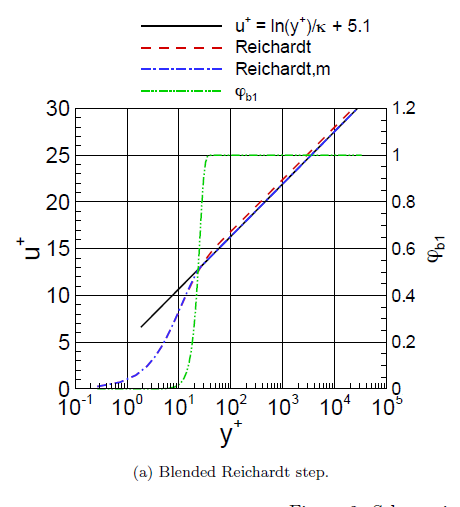
\includegraphics[width= 5cm]{Fun3D_v.png}
	\caption{RANS direct integration of the equations vs the Knopp proposal (figure from \cite{Knopp2007}).}
\end{figure}

For now, the boundary conditions that are implemented in TrioCMFD are equations \eqref{velocity_0} and \eqref{velocity_Knopp}.

\subsubsection{Turbulent kinetic energy}


Kalitzin et. al. \cite{Kalitzin2005} give a complete overview of the possible boundary conditions on the turbulent kinetic energy. Inside the viscous sublayer, the boundary condition on $k$ is:
\begin{equation}\label{eq_k_visc}
	k_{visc} = 0
\end{equation}

In the log-law region, the boundary condition is:
\begin{equation}\label{eq_k_log}
	k_{+,log} = 1/\sqrt{\beta_k}
\end{equation}

One of the often used proposals is:
\begin{equation}\label{eq_k_0}
	\partial_y k =0
\end{equation}

However, there is no universally accepted blending function. Another proposal is to use the relation $\nu_{t+} = \partial_{u_+}y_+ - 1$, but this has not been validated in a commercial code. This would yield:
\begin{equation}
	k_+ = \nu_{t+}\omega_+ = (\partial_{u_+}y_+ - 1) \omega_+
\end{equation}
\begin{equation}\label{eq_k_weak}
	\partial_y k_+ = (\partial_{u_+}y_+ - 1) \frac{u_\tau^2}{\nu} \partial_y \omega 
	- \frac{u_\tau}{\nu}\frac{\partial_{y_+}^2 u_+}{(\partial_{y_+}u_+)^2} \omega_+
\end{equation}

The formulations in equations $\eqref{eq_k_visc}$ and $\eqref{eq_k_0}$ are implemented in TrioCMFD. \\

Another simple boundary condition is a home-made transition from the viscous boundary condition to the zero-flux boundary condition by imposing a flux at the wall:
\begin{equation}\label{eq_k_blending}
	\Phi_{k, wall} = (\nu_l + \nu_t)/y \cdot (1-\tanh((y_+/20)^2))
\end{equation}

Finally, a boundary condition of equation \ref{eq_k_weak} is implemented with an imposed $k$ flux (see \cite{Mierka2007} for details on weak wall laws).

\subsubsection{Turbulent dissipation rate $\omega$}

The treatment of $\omega$ at the wall is one of the difficulties of $k-\omega$ models, as $\omega\rightarrow+\infty$ at the wall. \\

Wilcox recommends to input the values of $\omega$ in the first element by using the theoretical value of the viscous sub-layer: 
\begin{equation}
	\omega_\text{element} = \frac{6\nu}{\beta_\omega y^2}
\end{equation}

The boundary condition recommended by Menter in an SST $k-\omega$ \cite{Menter1993} is at the wall: 
\begin{equation}
	\omega_\text{wall} = 10 \frac{6\nu}{\beta_\omega y^2}
\end{equation}

Knopp proposed a blending function between the viscous and log-law regimes to obtain of $\omega$ \cite{Knopp2007}:

\begin{equation}
	\phi = \text{tanh}\left[\left(\frac{y_+}{10}\right)^2\right]
\end{equation}
\begin{equation}
	\omega_{vis} = \frac{6\nu}{\beta_\omega y^2}
\end{equation}
\begin{equation}
	\omega_{log} = \frac{u_\tau}{\sqrt{\beta_k}\kappa y}
\end{equation}
\begin{equation}
	\omega_{1} = \omega_{vis}+\omega_{log}
\end{equation}
\begin{equation}
	\omega_{2} =(\omega_{vis}^{1.2}+\omega_{log}^{1.2})^{1/1.2}
\end{equation}

\begin{equation}\label{eq_omega_Knopp}
	\omega = \phi \omega_{1} + (1-\phi) \omega_{2}
\end{equation}

They also recommend to enforce the theoretical value of $\omega$ in the first element. This is also what is done in \cite{Fun3D2015}. \\

\begin{figure}[h]
	\centering
	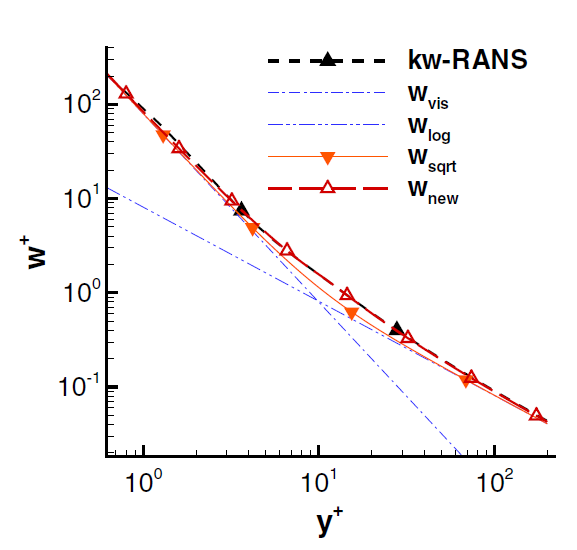
\includegraphics[width= 5cm]{Knopp_omega.png}
	\caption{RANS direct integration of the equations vs the Knopp proposal (image from \cite{Knopp2007}).}
\end{figure}

It is also possible to calculate the derivative of this theoretical value to obtain a flux to input in the first element:

\begin{equation}
	\partial_y\phi = \frac{u_\tau}{10\nu}\left(1-\text{tanh}\left[\left(\frac{y_+}{10}\right)^4\right]^2\right)
\end{equation}
\begin{equation}
	\partial_y\omega_{vis} = -\frac{12\nu}{\beta_\omega y^3}
\end{equation}\begin{equation}
	\partial_y\omega_{log} = - \frac{u_\tau}{\sqrt{\beta_k}\kappa y^2}
\end{equation}
\begin{equation}
	\partial_y\omega_{1} = \partial_y\omega_{vis}+\partial_y\omega_{log}
\end{equation}
\begin{equation}
	\partial_y\omega_{2} =(\omega_{vis}^{1.2}+\omega_{log}^{1.2})^{1/1.2}
\end{equation}
\begin{equation} \label{eq_omega_weak}
	\partial_y\omega = \partial_y\phi \omega_{1} + \phi \partial_y\omega_{1} -\partial_y\phi \omega_{2} + (1-\phi) \partial_y \omega_{2}
\end{equation}

For now, the only boundary condition that is implemented is \eqref{eq_omega_weak}, but work is ongoing on other possible boundary conditions.

\subsubsection{Turbulent time scale $\tau$}

The simplest boundary condition on $\tau$ is:
\begin{equation}\label{eq_tau_0}
	\tau_{wall}=0
\end{equation}

This is used in \cite{NEK50002020} for example. \\

Another possibility is to enforce a weak boundary condition by using $\tau = \frac{1}{\omega}$. This gives us:
\begin{equation}\label{eq_tau_weak}
	\partial_y\tau = -\frac{\partial_y\omega}{\omega^2}
\end{equation}

For now, the boundary conditions implemented on tau are \eqref{eq_tau_0} and \eqref{eq_tau_weak}. Work is ongoing on other possible boundary conditions.

\subsubsection{Temperature}

The heat transfer coefficient that we have implemented is the one proposed by Kader \cite{Kader1981}. It is compatible with adaptive wall functions. It is based on experiments and was later confirmed by DNS \cite{Mitrovic2004}. It is valid in an range where $6\cdot10^{-3}\inf Pr<6\cdot4^{4}$, for $Pr_t\approx0.85$.

\begin{equation}
	\Gamma = \frac{10^{-2}(Pr y_+)^4}{1+5Pr^3y_+}
\end{equation}
\begin{equation}
	\beta = (3.85Pr^{1/3}-1.3)^2+2.12ln(Pr)
\end{equation}
\begin{equation}
	\theta_+ = Pr y_+ \text{exp}(-\Gamma) +\left\{ 2.12ln\left[(1+y_+)\frac{2.5(2-2y/D_h)}{1+4(1-2y/D_h)^2}\right]+\beta\right\}\text{exp}(-1/\Gamma)
\end{equation}

\begin{figure}[h]
	\centering
	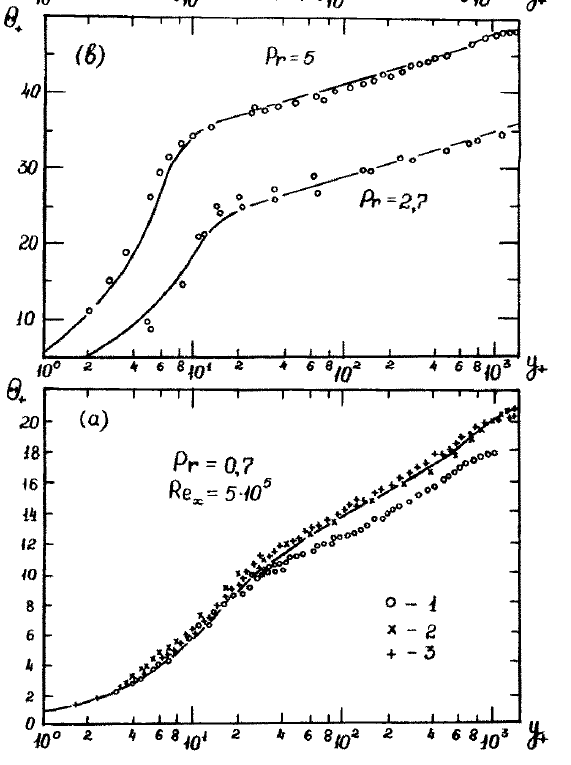
\includegraphics[width= 5cm]{Kader_T.png}
	\caption{Experimental results vs Kader forumala for different Prantl numbers (figure from \cite{Kader1981}).}
\end{figure}

\subsection{Description of the wall law algorithm implemented in TrioCMFD}

\subsubsection{Historic TrioCFD algorithm in VEF}

In VEF, the turbulent model used is $k-\epsilon$. The velocity is defined as a vector located at the center of the faces. Turbulent quantities (i.e. $k$ and $\epsilon$) as well. The information present in this subsection was determined by reading the source code.

For the velocity equation:
\begin{enumerate}
\item Calculate turbulent quantities at each face that is connected to a boundary element:
\begin{enumerate}
	\item Calculate $u_\parallel$ at the center of the face
	\item Calculate the friction viscosity $u_\tau$ using an iterative method that reconstructs the complete viscous sublayer, using $\frac{u_\parallel}{u_\tau} = u_+(\frac{y u_\tau}{\nu})$
	\item Calculate the shear stress $\tau_f = \rho u_\tau^2$
\end{enumerate}

\item Calculate the velocity diffusion terms:
\begin{enumerate}	
	\item Calculate the velocity diffusion for a $u=0$ boundary condition on the whole domain
	\item In the boundary elements, retract from the velocity diffusion the (viscosity * velocity gradient)  at the boundary face terms. Input the shear stress calculated with the wall law instead.
\end{enumerate}

\item Iterate one time step of the momentum equation

\item Update the turbulent quantity boundary conditions:
\begin{enumerate}
	\item Iterate one time step of the transport equation for $k$ and $\epsilon$.
	\item Use the equations on the turbulent quantities presented above to determine $\epsilon(y)$ and $k(y)$ at the faces connected to boundary elements.
	\item Input them in said faces at the end of each iteration (during the iterations, they are free to move as TrioCFD isn't designed to fix values inside elements or on faces as this would create a specific treatment for some internal faces and elements).
\end{enumerate}
\end{enumerate}

In VEF, the temperature is also located at the faces. To calculate the temperature diffusion, TrioCFD uses a separate equation to calculate the turbulence on temperature, recalculating $u_\tau$, $k$ and $\epsilon$ at the faces connected to a boundary element. Usually a Prandtl turbulence model is used to save calculation costs. When $k-\epsilon$ is used:
\begin{enumerate}
	\item Calculate $u_\tau$ in the faces connected to a boundary edge as for the velocity equation
	\item Calculate an equivalent distance to the edge using $u_tau$ to have the right heat flux while still using $T_{\text{wall}}$ at the edge in the diffusion operator.
	\item Iterate one time step of the conservation equation on the temperature.
	\item Iterate the equations for $k$ and $\epsilon$ as above.
\end{enumerate} 

\subsubsection{Fun3D algorithm}

See \cite{Fun3D2015}.

\begin{enumerate}
	\item Calculate $u_\parallel$
	\item Calculate the friction viscosity $u_\tau$ using Newton's method, using $\frac{u_\parallel}{u_\tau} = u_+(\frac{y u_\tau}{\nu})$
	\item Calculate the shear stress $\tau_f = \rho u_\tau^2$
	\item Obtain the momentum flux from the wall $-\tau_f \overrightarrow{t}$
	\item No heat transfer
	\item Turbulent quantities BL: it seems $\omega_{\text{element}} = \omega_{theorical}$ from equation \eqref{eq_omega_Knopp}, $k{\text{wall}} = 0$ are used (unclear in the paper)
\end{enumerate}

\subsubsection{TrioCMFD algorithm}

\begin{enumerate}
	\item Calculate $u_\parallel$
	\item Calculate the friction viscosity $u_\tau$ using dichotomic algorithm, using $\frac{u_\parallel}{u_\tau} = u_+(\frac{y u_\tau}{\nu})$
	\item Calculate the shear stress $\tau_f = \rho u_\tau^2$
	\item Obtain a friction coefficient at the wall $\alpha = \tau_f / u_\parallel$ that will be used to calculate the momentum flux
	\item Use the equation on the turbulent heat flux presented above to determine $q_{\text{wall}\rightarrow\text{phase~}n}$
	\item Calculate one of the following BC's on $k$:
	\begin{itemize}
		\item Use the equations on the turbulent quantities presented above to determine $\partial_y k(y)$ and use it as Neumann BC
		\item Use $k=0$
		\item Use $\partial_y k=0$
		\item Use equation \eqref{eq_k_blending}
	\end{itemize} 
	\item Either:
	\begin{itemize}
		\item Calculate one of the following BC's on $\omega$:
		\begin{itemize}
			\item Use the equations on the turbulent quantities presented above to determine $\partial_y \omega(y)$ and use it as Neumann BC
		\end{itemize}
		\item Calculate one of the following BC's on $\tau$:
		\begin{itemize}
			\item Use the equations on the turbulent quantities presented above to determine $\partial_y \tau(y)$ and use it as Neumann BC
			\item Use $\tau = 0$
		\end{itemize}
	\end{itemize}
	\item Iterate one time step of the complete system of equations (momentum, mass, energy, pressure, turbulent quantities)
\end{enumerate}

\subsection{Implementation for multiphase flows}

The implementation of shear-induced turbulence for single-phase flows was done by adding the liquid fraction $\alpha_l$ as a factor in all conservation equations for turbulent quantities. For example, equation \ref{eq_tau} becomes:

\begin{equation}
\begin{split}
	\partial_t { \alpha_l } \rho_l k + \nabla \cdot ({ \alpha_l } \rho_l k \vec{u_l}) 
	= & { \alpha_l } \underline{\underline{\tau_R}}::\underline{\underline{\nabla}}\vec{u_l} 
	- \frac{\beta_{k}{ \alpha_l }\rho k}{\tau}
	+ \nabla( { \alpha_l } \rho_l(\nu_l + \sigma_k \nu_t) \underline{\nabla} k)
	\\
	\partial_t { \alpha_l } \rho_l \tau + \nabla \cdot ({ \alpha_l } \rho_l \tau \vec{u_l}) 
	= &	- \alpha_{\omega} { \alpha_l } \frac{\tau}{k}\underline{\underline{\tau_R}}::\underline{\underline{\nabla}}\vec{u_l}
	+ \beta_{\omega}{ \alpha_l }\rho
	+\nabla( { \alpha_l } \rho_l(\nu_l + \sigma_{\omega} \nu_t) \underline{\nabla} \tau) \\
	& - 8 { \alpha_l } \rho_l(\nu_l + \sigma_{\omega} \nu_t) ||\underline{\nabla}\sqrt{\tau}||^2
	+ \sigma_d { \alpha_l } \rho_l \tau \text{min}\left\{\underline{\nabla}k \cdot \underline{\nabla} \tau, 0\right\}
\end{split}
\end{equation}

\section{Multiphase CFD in TrioCFMD}

TrioCMFD uses the PolyMAC numerical scheme \cite{Gerschenfeld_PolyMAC2018, Gerschenfeld_PolyMAC2022}. This scheme was initially developed for multiphase component scale codes. TrioCMFD is based on a 2-fluid 6-equation Euler-Euler framework called Pb\_Multiphase. The resolution of the equations is done using semi-implicit ICE and SETS solvers that are located in TRUST. TrioCMFD regroups interfacial terms that are specific to CFD applications. This includes interfacial forces, energy transfer, wall heat flux partitioning, bubble diameter determination... \\

Work is still being done on the models presented in this section, and they are not fully validated.

\subsection{Definition of dimensionnal and dimensionless variables}

\begin{center}
\begin{tabular}{|r|l|}
	\hline Variable name & Expression \\ \hline \hline
	Vapor phase & $v$ \\ \hline
	Liquid phase & $l$ \\ \hline
	Distance to the wall & $y$ \\ \hline
	Normal unit vector from the wall & $\overrightarrow{n}$ \\ \hline
	Velocity of phase k & $\overrightarrow{u_k}$\\ \hline
	Dynamic viscosity of phase k
		& $\mu_k $ \\ \hline
	Volume mass of phase k
		& $\rho_k$ \\ \hline
	Kinematic viscosity of phase k
		& $\nu_k = \mu_k/\rho_k$ \\ \hline
	Turbulent dynamic viscosity of the carrying phase
		& $\mu_{t} $ \\ \hline
	Turbulent kinematic viscosity of the carrying phase
		& $\nu_t = \mu_t/\rho$ \\ \hline
	Reynold's stress tensor of the carrying phase
		& $\underline{\underline{\tau_R}} = - <u_iu_j>$ \\ \hline
	Turbulent kinetic energy of the carrying phase
		& $k$ \\ \hline
	Turbulent kinetic energy dissipation of the carrying phase
		& $\epsilon$ \\ \hline	
	Temperature of phase k
		& $T_{k}$ \\ \hline
	Temperature of the wall
		& $T_\text{wall}$ \\ \hline
	Thermal conductivity of phase k
		& $\lambda_k =$ \\ \hline
	Heat capacity at constant volume of phase k
		& $Cp_k$ \\ \hline
	Forced convection heat transfer coefficient
		& $h_{fc}$	\\ \hline
	Liquid fraction 
		& $\alpha_l $ \\ \hline
	Void fraction 
		& $\alpha_v $ \\ \hline
	Internal energy of phase k
		& $e_k $ \\ \hline
	Mass transfer to phase k
		& $\Gamma_k $ \\ \hline
	Mass transfer to phase k
		& $\Gamma_k $ \\ \hline
	Interfacial forces applied to phase k
		& $\vec{F}_{ki}$  \\ \hline
	Volume forces applied to phase k (i.e. gravity)
		& $\vec{F}_k$  \\ \hline
	Interfacial heat flux to phase k
		& $q_{ki}$ \\ \hline
	Wall heat flux to phase k
		& $q_{kp} $ \\ \hline
	Interfacial area between phase $l$ and $v$
		& $a_i$ \\ \hline
	Bubble diameter of phase $v$
		& $	d_b = \frac{6 \alpha_v}{a_i} $ \\ \hline
	Bubble nucleation and departure from wall diameter
		& $d_\text{dep}$ \\ \hline
	Vapor/liquid saturation temperature
		& $T_\text{sat}$ \\ \hline
	Vapor/liquid latent heat
		& $L_\text{vap}$ \\ \hline
	Vapor/liquid surface tension
		& $\sigma$ \\ \hline
	Percentage of wall surface occupied by sliding bubbles
		& $S_{sl}$ \\ \hline
	Bubble Reynold's number
		& $Re_b = \frac{||\overrightarrow{u_v}-\overrightarrow{u_l}|| d_b}{\nu_l}$ \\ \hline
	Bubble turbulent fluctuation Weber number
		& $We = \frac{(\epsilon d_b)^{2/3} \rho_l d_B}{\sigma}$ \\ \hline
	Eotvos number
		&  $Eo = \frac{g(\rho_l-\rho_v)d^2}{\sigma}$ \\ \hline
	Turbulent Prandtl number of the liquid 
		& $Pr_t \sim 1 $ \\ \hline
	Superheat Jacob number
		& $Ja_\text{sup} = \frac{\rho_l Cp_l \cdot (T_\text{wall} - T_\text{sat})}{\rho_v L_\text{vap}}$ \\ \hline
	Subcooling Jacob number	
		& $Ja_\text{sub} = \frac{\rho_l Cp_l \cdot (T_\text{sat} - T_l)}{\rho_v L_\text{vap}}$ \\ \hline


\end{tabular}
\end{center}
\pagebreak

\subsection{2-fluid 6-equation framework}

TrioCMFD is based on the Pb\_Multiphase framework that was originally developed for component scale codes \cite{Gerschenfeld_PolyMAC2018, Gerschenfeld_PolyMAC2022}.
This framework contains the multiphase terms that are common to component scale codes and CFD, that we do not need to add in TrioCMFD. 
Equation \eqref{eq_6} presents the terms that are already included in TRUST and the terms that we have added TrioCMFD.

\begin{equation} \label{eq_6}
	\begin{array}{c r c l}
		(\mathcal{M}_k) 
		& \underbrace{\frac{\partial  \alpha_k \rho_k}{\partial t} + \nabla \cdot ({\alpha_k \rho_k} \vec{u_k})}_\text{TRUST}
		& =
		& \underbrace{\Gamma_k}_\text{\blue TrioCMFD}
		\\
		(\mathcal{Q}_k) 
		& \underbrace{\frac{\partial \alpha_k \rho_k \vec{u_k}}{\partial t} + \underline{\nabla} \cdot ({\alpha_k \rho_k \vec{u_k}} \otimes \vec{u_k})}_\text{TRUST}
		& =
		& \underbrace{-\alpha_k \underline{\nabla} P}_\text{TRUST} +
		\underline{\nabla} \cdot [ \underbrace{\alpha_k \mu_k \underline{\underline{\nabla}} \vec{u_k}}_\text{TRUST} \underbrace{- \alpha_k\rho_k \overline{u_i'u_j'}}_\text{\blue TrioCMFD}]
		\underbrace{+ \vec{F}_{ki}
		+ \vec{F}_k}_\text{\blue TrioCMFD}
		\\
		(\mathcal{E}_k) 
		& \underbrace{\frac{\partial \alpha_k \rho_k e_k}{\partial t} + \nabla \cdot ({\alpha_k \rho_k h_k} \vec{u_k})}_\text{TRUST}
		& =
		& \nabla \cdot [ \underbrace{\alpha_k\lambda_k \underline{\nabla} T_k}_\text{TRUST}  \underbrace{- \alpha_k\rho_k \overline{u_i'e_k'}}_\text{\blue TrioCMFD} ] 
		\underbrace{-p \left[\frac{\partial \alpha_k}{\partial t} + \nabla \cdot (\alpha_k u_k)\right]}_\text{TRUST} +
		\underbrace{q_{ki} +
		q_{kp}}_\text{\blue TrioCMFD}
		
	\end{array}
\end{equation}

The implementation of single-phase turbulence is treated in a separate section (terms $\underline{\nabla} \cdot [ - \alpha_k\rho_k \overline{u_i'u_j'}]$ and  $\underline{\nabla} \cdot [ - \alpha_k\rho_k \overline{u_i'e_k'}]$). \\

One physical quantity that is necessary for the implementation of multiphase terms is the bubble diameter. Section \ref{seq_diameter} presents the possibilities in CMFD. The other sections present the implementation of interfacial forces, two-phase turbulence,  interfacial heat transfer and heat flux partitioning.

\subsection{Determination of bubble diameter}
\label{seq_diameter}

\subsection{Constant diameter}

The first closure for the bubble diameter is to fix a single constant diameter to all elements in the system. \\

\subsubsection{User-defined or experimental diameter field}

Inspired by \cite{Sugrue2017, Sugrue2017a}, we also wanted to fix an experimentally determined diameter. The TRUST field framework can be used to fix a bubble diameter field. This gives the user different possibilities:
\begin{itemize}
	\item A constant field (redundant with the constant diameter)
	\item A field that is a function of (x, y, z) coordinates and/or time
	\item A field that can be inputted from an data file
\end{itemize}

\subsubsection{1-group interfacial area transport equation}

Finally, we implemented the one-group interfacial area transport model proposed by Yao and Morel for nuclear applications \cite{Yao2004}. The interfacial area $a_i$ is a volume density of area and is therefore in $m^{-1}$. The governing equations of this model are:

\begin{equation}
	\partial_t a_i 
	\underbrace{+ \overrightarrow{u} \cdot \underline{\nabla}(a_i)}_\text{Convection} 
	= \frac{2}{3} \frac{a_i}{\alpha_v} 
		\left( \underbrace{\frac{\Gamma_v}{\rho_v}}_\text{Condensation} 
			   \underbrace{- \alpha_v\frac{\partial_t \rho_v}{\rho_v}}_{\Delta \rho } \right) 
	\underbrace{+ \pi d_\text{dep}^2 \Phi_N }_\text{Nucleation} 
	+ \frac{36 \pi}{3} \left(\frac{\alpha}{a_i}\right)^2 
		( \underbrace{\Phi_{Coal} }_\text{Coalescence}
		+ \underbrace{\Phi_{Bkp}  }_\text{Breakup} )
\end{equation}

The phenomena taken into account in this equation are:
\begin{itemize}
	\item \textbf{Convection}
	\item \textbf{Condensation}: $\Gamma_v$ is the phase transfer term. The expression $\frac{2}{3} \frac{a_i}{\alpha_v} \frac{\Gamma_v}{\rho_v} $ allows us to take into account the change of bubble radius due to condensation or evaporation.
	\item \textbf{$\Delta \rho$}: the expression $- \frac{2}{3} \frac{a_i}{\alpha_v} \alpha_v\frac{\partial_t \rho_v}{\rho_v} $ allows us to take into account the change of bubble radius due to a change of volume mass, due to pressure and temperature variations.
	\item \textbf{Nucleation}: $d_\text{dep}$ is the nucleation diameter of the bubbles at the wall. This is calculated inside the wall heat transfer model. Another output of this model is the evaporative wall heat transfer $\Phi_{e}$ (in $Wm^{-2}$). $\Phi_N$ can be determined using :
	\begin{equation}
		\Phi_{N} 
		=
		\frac{\Phi_{e}}{L_\text{vap} \cdot \rho_v \cdot\frac{\pi}{6}d_\text{dep}^3}
	\end{equation}
	\item \textbf{Coalescence}: $\Phi_{Coal}$ is the number of coalescing bubbles by second by unit volume. Along with the breakup term, this is the main difference between one-group interfacial area frameworks. The formulation proposed by Yao and Morel is:
	\begin{equation}
		\Phi_{Coal} = - (\epsilon d_b)^{1/3} \cdot \frac{\alpha_v^2}{d_b^4} \cdot K_{c1} \cdot \frac{1}{g(\alpha_v) + K_{c2}\alpha_v \sqrt{We/We_{cr}}} \cdot \text{exp}\left(-K_{c3} \sqrt{\frac{We}{We_{cr}}}\right)
	\end{equation}
	Where $d_b = \frac{6 \alpha_v}{a_i} $ is the average bubble diameter, $K_{c1} = 2.86$, $K_{c2} = 1.922$, $K_{c3} = 1.017$, $We_{cr} = 1.24$, $g(\alpha) = \frac{\alpha_\text{max}^{1/3}-\alpha^{1/3}}{\alpha_\text{max}^{1/3}}$, $\alpha_\text{max}^{1/3} = \pi/6$.
	\item \textbf{Breakup}: $\Phi_{Bkp}$ is the number of bubbles that breakup by second by unit volume. Along with the coalescence term, this is the main difference between one-group interfacial area frameworks. The formulation proposed by Yao and Morel is:
	\begin{equation}
	\Phi_{Bkp} = (\epsilon d_b)^{1/3} \cdot \frac{\alpha_v(1-\alpha_v)}{d_b^4} \cdot K_{b1} \cdot \frac{1}{1 + K_{b2}(1-\alpha_v) \sqrt{We/We_{cr}}} \cdot \text{exp}\left(- \frac{We}{We_{cr}}\right)
	\end{equation}
	Where $d_b = \frac{6 \alpha_v}{a_i} $, $K_{b1} = 1.6$, $K_{b2} = 0.42$, $We_{cr} = 1.24$.
	
\end{itemize}

More coalescence and fragmentation models will certainly be available in the future. The other terms of the equation are generic and common to all 1-group interfacial area transport models.


\subsection{Interfacial forces}

In this section, the expression given is the force acting on the gas phase. The opposite force acts on the liquid phase.

\subsubsection{Drag}

The general formulation for a drag force is of the form:

\begin{equation}
\overrightarrow{F_{l\rightarrow v}}= - \frac{3}{4} C_D \frac{\alpha_v\rho_l}{d_b} ||\overrightarrow{u_v}-\overrightarrow{u_l}|| (\overrightarrow{u_v}-\overrightarrow{u_l})
\end{equation}

The drag coefficient that is implemented is the Tomiyama drag 
\cite{Tomiyama1998}:

\begin{equation}
C_D = \begin{cases} \max(\min(16/Re_b(1+.15Re^{.687}), 48/Re_b), 8Eo/(3+12)) \text{, No contamination}\\
	\max(\min(24/Re_b(1+.15Re^{.687}), 72/Re_b), 8Eo/(3Eo+12)) \text{, Slight contamination}\\
	\max(~~~~~~24/Re_b(1+.15Re^{.687}), ~~~~~~~~~~~~8Eo/(3Eo+12)) \text{, High contamination} \end{cases}
\end{equation}

Where $Eo = \frac{g(\rho_l-\rho_v)d^2}{\sigma}$. This formulation was chosen as, as shown in \cite{Sugrue2017}, it yields similar results as other closures and one can adjust the level of contamination.

\subsubsection{Lift}

The general formulation for a drag force is of the form:

\begin{equation}
	\overrightarrow{F_{l\rightarrow v}}= - C_L \rho_l \alpha_v (\overrightarrow{u_v}-\overrightarrow{u_l}) \wedge \overrightarrow{u_l}
\end{equation}

The lift coefficient that is implemented is the Tomiyama lift \cite{Tomiyama2002}:

\begin{equation}
	C_L = \begin{cases} \min(.288\tanh(.121Re_b),f(Eo)) \text{,~} Eo<4 \\ f(Eo) \text{,~} 4 \leq Eo \leq 10.7 \end{cases}
\end{equation}

Where $f(Eo) = .00105Eo^3 - .0159Eo^2 - .0204 Eo + .474$.

\subsubsection{Dispersion}

The bubble dispersion formulation implemented is the one proposed by Burns et al. \cite{Burns2004}:

\begin{equation}
\vec{F}_{l\rightarrow v} = -\frac{3}{4} \frac{C_D}{d_b}\alpha_v|\vec{u_g}-\vec{u_l}|\frac{\mu_{\text{turb}}}{Pr_{\alpha\text{, turb}}}
\left(\frac{\underline{\nabla}\alpha_v}{\alpha_v}-\frac{\underline{\nabla}\alpha_l}{\alpha_l}\right)
\end{equation}

Where $Pr_{\alpha\text{, turb}}=1$

\subsubsection{Wall correction}

The wall correction term implemented is the one proposed by Lubchenko et al. \cite{Lubchenko2018}. Is is based on geometrical arguments. It consists in modifying the lift coefficient and the dispersion close to the wall.

Close to the wall, the lift coefficient becomes:
\begin{equation}
	C_L \rightarrow \begin{cases} 0 \text{,~} y/d_B<1/2  \\
	C_L\left(3\left(\frac{2y}{d_B}-1\right)^2-2\left(\frac{2y}{d_B}-1\right)^3\right) \text{,~} 1/2 \leq y/d_B < 1 \\
	C_L \text{,~} y/d_B\geq 1 \end{cases}
\end{equation}

The expression of the turbulent dispersion force is modified by replacing $\underline{\nabla}\alpha_v$ by:
\begin{equation}
	 \underline{\nabla}\alpha_v \rightarrow \alpha_v\frac{1}{y}\frac{d_B-2y}{d_B-y}\overrightarrow{n}
\end{equation}

\subsubsection{Tchen}

The Tchen force \cite{Tchen1947} is implemented with the following expression:

\begin{equation}
\overrightarrow{F_{l\rightarrow v}}= \alpha_v\rho_l \partial_t \overrightarrow{u_l}
\end{equation}

\subsection{Two-phase turbulence}

By two-phase turbulence, we mean the effect of the bubbles on the turbulence in the liquid phase. To model this, we implemented the models developed during the PhD of Antoine Ducluzeau \cite{DuCluzeau2019, Cluzeau2019, Cluzeau2019a}. The authors divide the velocity fluctuations caused by the movement of bubbles in the fluid in two parts: wake-induced turbulence and wake-induced fluctuations. The total Reynolds stress tensor is the sum of all single-phase (calculated using 2-equation turbulence models) and two-phase turbulence.

\begin{equation}
		\underline{\underline{\tau_R}} 
		=\underline{\underline{\tau_R}}_{\text{single-phase}}
		+ \underline{\underline{\tau_R}}_{\text{WIF}}
		+ \underline{\underline{\tau_R}}_{\text{WIT}}
\end{equation}

\subsubsection{Wake-induced turbulence} 

Wake-induced turbulence is the isotropic contribution of bubbles to the velocity fluctuations. It comes from the instabilities of bubble wakes. It takes the shape of an additional transport equation for the bubble-induced turbulent kinetic energy $k_{WIT}$.

\begin{equation}
	\underline{\underline{\tau_R}}_{\text{WIT}}
	= k^{WIT}\frac{2}{3}\delta_{ij}
\end{equation}
\begin{equation}
				\frac{D k^{WIT}}{DT} = 
				\underbrace{C_D\nabla^2 k^{WIT} }_\text{Diffusion} 
				\underbrace{ - \frac{2 \nu_l C_D' Re_b}{C_\Lambda^2 d_b^2}k^{WIT} }_\text{Dissipation}
				+ \underbrace{\alpha_v \frac{(\rho_l-\rho_v)}{\rho_l} g |\vec{u_v}-\vec{u_l}|\left(0.9 - exp\left(-\frac{Re_b}{Re_b^c}\right)\right) }_\text{Production}
\end{equation}

Where $C_\Lambda = 2.7$, $Re_b^c = 170$, $C_D'$ is a user-inputted drag coefficient $C_D$ is a turbulent diffusion coefficient.

\subsubsection{Wake-induced fluctuations} 


Wake-induced fluctuations are the anisotropic effects of the average wake. These fluctuations are primarily in the direction of the liquid-gas velocity difference, i.e. in the vertical direction. No transport equation is necessary to model this term.
\begin{equation}
	\underline{\underline{\tau_R}}_{\text{WIF}} =
	\alpha_v |\overrightarrow{u_v}-\overrightarrow{u_l}|^2
	\begin{bmatrix}
		3/20 & 0 & 0 \\
		0 & 3/20 & 0 \\
		0 & 0 & 1/5+3C_v/2
	\end{bmatrix}
\end{equation}

Where $C_v = 0.36$.

\subsection{Interfacial heat transfer}

The Ranz-Marshall model \cite{RanzMarshall1952} for interfacial heat transfer is the only one implemented in the code for now:

\begin{equation}
	q_{ki} = \frac{6\alpha_v\lambda_l}{d_b^2}\left(2+0.6\left(\frac{d_b||\vec{u_l}-\vec{u_v}||}{\mu_l}\right)^{1/2}\left(\frac{\mu_l Cp_l}{\lambda_l}\right)^{1/3}\right)(T_v-T_l)
\end{equation}

This formulation has many shortcomings and work is ongoing to select and implement better closures.

\subsection{Heat flux partitioning}

The model for the wall heat flux partitioning in nucleate boiling regime implemented is the one developed by Kommajosyula during his PhD thesis \cite{Ravik2020}.

In this model, the wall heat flux is separated in 3 distinct contributions:

\begin{equation}
	\Phi_{NB}
	=
	\underbrace{\Phi_{fc}}_\text{convection}
	+
	\underbrace{\Phi_{sc}}_\text{sliding}
	+
	\underbrace{\Phi_{e}}_\text{evaporation}
\end{equation}

\subsubsection{Intermediate quantities that require computing}

\textbf{Jacob numbers} are the first computed quantities. We have, for the superheating and subcooling numbers respectively:
\begin{equation}
	Ja_\text{sup} = \frac{\rho_l Cp_l \times (T_\text{wall} - T_\text{sat})}{\rho_v L_\text{vap}}
\end{equation}

\begin{equation}
	Ja_\text{sub} = \frac{\rho_l Cp_l \times (T_\text{sat} - T_l)}{\rho_v L_\text{vap}}
\end{equation}

\textbf{Departure diameter} is then calculated using the following correlation fitted by the authors:

\begin{equation}
	d_\text{dep}
	=
	18.9 \cdot 10^{-6}
	\times
	\left(\frac{\rho_l-\rho_v}{\rho_v}\right)^{0.27}
	\times
	Ja_\text{sup}^{0.75}
	\times
	(1+Ja_\text{sub})^{-0.3}
	\times
	u_l^{-0.26}
\end{equation}

A \textbf{bubble growth constant} is calculated to later determine the growth time (for now we ignore the contribution of microlayer evaporation):
\begin{equation}
	K
	=
	\left(1.55 - 
	0.05 \cdot \frac{T_\text{wall}-T_\text{sat}}{T_\text{sat}-T_l}\right)
	\times
	2 \cdot \sqrt{3/\pi}
	\times
	Ja_\text{sup}
	\times
	\frac{\lambda_l}{\rho_l Cp_l}
\end{equation}

\textbf{Bubble growth time} is calculated using the two previous quantities:
\begin{equation}
	t_\text{growth}
	=
	\left(\frac{d_\text{dep}}{4K}\right)^2
\end{equation}

\textbf{Bubble wait time} is calculated using the following correlation fitted by the authors:
\begin{equation}
	t_\text{wait}
	=
	\frac{0.0061 \times Ja_\text{sub}}{T_\text{wall}-T_\text{sat}}
\end{equation}

The \textbf{time to reform the thermal boundary layer} is calculated as:
\begin{equation}
	t_{BL} = \frac{\lambda_l^2}{h_{fc}^2 \pi \nu_l}
\end{equation}
N. B.: this formulation is a correction of the one present in equation (4.5) of \cite{Ravik2020}.\\

\textbf{Bubble departure frequency} is therefore:
\begin{equation}
	f_\text{dep}
	=
	\frac{1}{t_\text{wait} + t_\text{growth}}
\end{equation}

The \textbf{nucleation site density} $N''$ is calculated using the 2003 Hibiki-Ishii model \cite{Hibiki2003}. \\

The \textbf{active site density} is a correction of $N''$ that takes into account the suppression of some sites by others by using a Lambert's function. An approximation proposed in \cite{Ravik2020} gives:
\begin{equation}
	N''_a = 
	\begin{cases}
		N'' & \text{for~} N_0 N'' < e^{-1} \\
		\frac{0.2689 N_0 N'' + 0.2690}{N_0} 
			& \text{for~} e^{-1} \leq N_0 N'' < e \\
		\frac{\text{log}(N_0 N'') - \text{log}(\text{log}(N_0 N''))}{N_0}
			& \text{for~} < e \leq  N_0 N'' \\
	\end{cases}
\end{equation} 
Where $N_0 = f_\text{dep} t_\text{growth} \pi (d_\text{dep}/2)^2$. \\

The \textbf{bubble sliding area} of a single bubble is then given by:
\begin{equation}
	A_{sl} = \frac{1}{\sqrt{N_a''}} d_\text{dep}
\end{equation}
Using $\frac{1}{\sqrt{N_a''}}$ as the average distance between two nucleation sites.\\

The \textbf{sliding surface occupation} can then finally be computed:
\begin{equation}
	S_{sl} = \text{min}(1, A_{sl} N_a'' f_\text{dep} t_{BL} )
\end{equation}

\subsubsection{Convection}

\begin{equation}
	\Phi_{fc}
	=
	\underbrace{(1-S_{sl})}_\text{\% free surface}
	\times
	h_{fc}
	\times
	(T_\text{wall}-T_\text{liquid})
\end{equation}

Where $h_{fc}$ is calculated using the Kader adaptive temperature wall law \cite{Kader1981}.

\subsubsection{Sliding}

Sliding acts as an enhancement of the single-phase forces convection:

\begin{equation}
	\Phi_{sl}
	=
	2 S_{sl}
	\times
	h_{fc}
	\times
	(T_\text{wall}-T_\text{liquid})
\end{equation}

\subsubsection{Evaporation}

The heat transfer due to evaporation is:
\begin{equation}
	\Phi_{e}
	=
	\frac{\pi}{6}
	\cdot
	\rho_v
	\cdot
	L_\text{vap}
	\cdot
	d_\text{dep}^3
	\cdot
	f_\text{dep}
	\cdot
	N''_a
\end{equation}

\section{Homogeneous Equilibrium Model}
\label{sec:homog-equil-model}

\textit{Disclaimer: this documentation is a very short, incomplete and
inaccurate introduction to the modelling of an homogeneous equilibrium
model in TrioCFD. Being a work in progress, this documentation will be
revised in a near future.}

The CMFD baltik gathers the development of the multiphase CFD in
TrioCFD. This approach designates all RANS approaches for multiphase
flows. It is based on the Pb\_Multiphase problem. The model uses
instantaneous relaxation of a fully unequilibrated model rather than a
direct approach as in \cite{Goncalves2009}.\\
The Homogeneous Equilibrium Model (HEM hereafter) is an approximation
of a multiphase flow where the phases are mechanically and thermally
coupled. They move at the same velocity and have the same temperature
which may not be their saturated temperature if the fluids are not of
the same type.

\subsection{The non-viscous system of equation}
\label{sec:non-viscous-system}



A non viscous two-phase flow can be describe by Euler's equations
where every thermodynamical variable in the system describes the
mixing as the sum of each phase's contributions:

\begin{align}
&\partial_t (\rho) +\partial_x (\rho u) = 0, \nonumber\\
%%%%%%%%%%%%%%%%%%%%%%%%%%%%%%V
&\partial_t (\rho u) +\partial_x (\rho u^2 + P) = 0, \nonumber\\
%%%%%%%%%%%%%%%%%%%%%%%%%%%%%%
&\partial_t (\alpha\rho E) +\partial_x (\rho uH) = 0,  \nonumber
\label{sistema1}
\end{align}

whit $E=e+\frac{u^2}{2}$ the total energy of the system and
$H=h+\frac{u^2}{2}$ the total enthalpy. $e$ et $h$ are the internal
energy and internal enthalpy of the mixing. They both depend on the
volume fraction and properties of each phase:

\begin{align}
\rho e&\triangleq\alpha_G \rho_G e_G + (1 -\alpha_G)\rho_L e_L \\
\rho h&\triangleq\alpha_G \rho_G h_G + (1 -\alpha_G)\rho_L h_L.
\end{align}

The mixing density $\rho$ is defined by:
\begin{equation}
\rho \triangleq \alpha_G\rho_G+(1-\alpha_G)\rho_L
\end{equation}
with $\rho_L$ and $\rho_G$ the liquid and gas densities, respectively.
The void fraction $\alpha_G$ stands for the \emph{attendance rate} of
the gaz phase. It is defined between 0 and 1.


The system unkowns are $\alpha_G$, $P_k$, $T_k$, $v_k$ et $\rho_k$,
but the applied simplification ($P_G=P_L$, $T_G=T_L$ et $v_G=v_L$) allows for a reduction of the number of
equations. To close the system, a equation of state (EOS) for each
phase is needed as well as a thermodynamics relationship for the
mixing between the system pressure, another thermodynamics variable
(temperature, enthalpy, or density), and the void fraction.

\subsection{The equation of state}
In this section, the different approach for the choice of the equation
of state are presented. They are all available in \texttt{Pb\_HEM}.

\subsubsection{Incompressible}

For the incompressible case, both densities are taken constant in each
phase.

\subsubsection{Quasi-compressible formulation}
For the quasi compressible case, the densities only depend on the
temperature. The following equations of state can thus be used for a
range of temperature between 50°C and 263°C~\cite{Rodio2019} :
\begin{equation}
\rho(T)=-0.0023864182 T^2-0.22507878 T + 1007.1165.
\label{loi_qc}
\end{equation}

\subsubsection{Compressible case}
A stiffened gas equation has been added to the code. It allows to
guarantee the hyperbolicity of the system as the sound velocity is
always positive, being squared. It is defined as follows:

\begin{align}
P(\rho ,e)&=(\gamma-1)\rho(e-q)-\gamma P_{\infty}\\
P(\rho ,T)&=\rho (\gamma-1)C_vT-\gamma P_{\infty}\\
T(\rho ,h)&=\frac{h-q}{C_p}\\
c^2&=\gamma\frac{P+P_{\infty}}{\rho},
\end{align}
with $\gamma=C_p/C_v$ the polytropique coefficient, $C_p$ and $C_v$
the calorimetric coefficients, and $P_{\infty}$ a constant reference pressure.

\subsubsection{More complex equations of state}
\label{sec:more-compl-equat}

More complex equations of state will be available in the near future
with the use of an library of equations of state (as the commercial
RefProp library for instance) through a in-house code.


\subsection{The Navier-stokes system of equations}
The complete system of equations is defined as follows:
% \begin{scriptsize}
\begin{equation}
% \left\{
% \begin{split}
%%%%%%%%%%%%%%%%%%%%%%%%%%%%%%
\partial_t (W) + \nabla (F_c-F_v) = S,
% \end{split}
% \right.
% \label{sistema2}
% \end{equation}
% \end{scriptsize}
\quad \mbox{où}\quad
% \begin{scriptsize}
% \begin{equation}
%%%%%%%%%%%%%%%%%%%%%%%%%%%%%%
W=\begin{pmatrix}
\rho\\
\rho U\\
\rho E\\
\varepsilon_{turb}
\end{pmatrix},
F_c=\begin{pmatrix}
\rho U\\
\rho V\bigotimes U\\
(\rho E +P)U\\
\varepsilon_{turb} U
\end{pmatrix},
F_v=\begin{pmatrix}
0\\
\bar{\bar{\tau^v}} +\bar{\bar{\tau^t}}\\
(\bar{\bar{\tau^v}} +\bar{\bar{\tau^t}})\cdot U-Q^v-Q^t\\
S_{turb}
\end{pmatrix}
\label{sistema4}
\end{equation}
% \end{scriptsize}
Source termes are added to the previous Euler system of equations. $W$
stands for the conservative variables, $F_c$ et $F_v$ for the
convective and viscous flux respectively, $S$ the sources terms, and
$\varepsilon_{turb}$ the turbulence model variables.

The viscous stress tensor $\bar{\bar{\tau}}$ can be defined following
the Boussinesq hypothesis.

Several turbulence model can be defined, as defined in the more
complete model.

\subsection{Drift-flux models}

The drift-flux model is an appropriate choice whenever the two-phase flow is strongly coupled, i.e. only small kinematic desequilibrium between the phases may appear \cite{hibiki2002distribution}. The system is then described by the mixture balance equations for mass, momentum and energy, supplemented by the formulation of a relative velocity that accounts for the kinematic desequilibrium between both phases. \\

Zuber and Findlay \cite{zuber1965average} introduced in 1965 a formulation of the void-fraction-weighted mean gas velocity (or intrinsic averaged gas velocity) as a function of the area-averaged mixture velocity : 

	\begin{equation}\label{eq_drift-velocity}
		\mathbf{V_g} = \frac{\left\langle\alpha_g * \mathbf{v_g}\right\rangle}{\left\langle\alpha_g\right\rangle} = C_0 \mathbf{J} + \mathbf{V_{gj}} 
	\end{equation}
	
	
where $\mathbf{V_g}$ is the void-fraction-weighted mean gas velocity, $C_0$ is the distribution parameter, $\mathbf{V_{gj}}$ the void-fraction-weighted mean drift velocity and $\mathbf{J}$ denotes the area-averaged mixture velocity. The latter is the volume average of the mixture local velocity $\mathbf{j}$, which can be expressed in terms of the local phase velocities $\mathbf{v_l}$ and $\mathbf{v_g}$ and the phase fractions $\alpha_l$ and $\alpha_g$ as follows:%$\left\langle\mathbf{j}\right\rangle$ the area-averaged mixture velocity defined as follows: 
	
	\begin{equation}
		\mathbf{j} = \alpha_g \mathbf{v_g} + \alpha_l \mathbf{v_l}
	\end{equation}
	
with $\mathbf{J} = \left\langle \mathbf{j} \right\rangle $ 


The constitutive equations for the drift-flux model, originally developed to calculate intrinsic averaged velocities in vertical upward two-phase flows \cite{zuber1965average}\cite{ishii1977one}, where later on extended at the local scale to three-dimensional and more complex flows \cite{manninen1996mixture}\cite{mahdavi2017implementation}, thereby allowing to define a local drift velocity in stream and transverse directions.\\

In TrioCFD, several drift velocities are proposed at the component and local scales. 

\paragraph{At the component scale } (i.e. nuclear core reactor, steam generator, ...), the porous medium is represented by an homogeneous equivalent medium and instrinsic average velocities are (amongst others) unknowns of the system. Two different drift-velocities may be chosen to close the system of equations:
\begin{itemize}
	\item Either the distribution parameter $C_0$ and the void-fraction-weighted mean drift velocity vector are used-defined constants. 
	\item Or fitted for the bubbly flow regime as proposed by  Hibiki and Ishii \cite{hibiki2002distribution} : 
	\begin{align}
		C_0 = \big(1.2 - 0.2 \sqrt{\frac{\rho_g}{\rho_l}}\big)(1-\exp(-18\left\langle\alpha_g\right\rangle))\\
		V_{gj} = \sqrt{2}\big(\frac{g\Delta\rho}{\rho_f^2}\big)^{1/4}(1-\left\langle\alpha_g\right\rangle)^{1.75},
	\end{align}

The vector $\mathbf{V_{gj}}$ is oriented in the stream direction. Let us recall that the drift-flux model established by \cite{hibiki2002distribution} is valid for one-dimensional upward two-phase flows. 
\end{itemize}

\paragraph{At the local scale} 
\begin{itemize}
	\item Either the distribution parameter $C_0$ and a local gas drift-velocity vector are used-defined constants. 
	\item Or the three-dimensional drift-velocity is derived as proposed by Manninen \cite{manninen1996mixture}. The dispersed phase (denoted by the subscript d) is assumed in equilibrium in the continuum phase (denoted by the subscript c) such that the force balance applied to the dispersed phase equates to zero, thereby leading to the formulation of the relative velocity in the stream and transverse direction :
	
	\begin{align}
		\mathbf{F_{FI}} = K ||\mathbf{u_d} - \mathbf{u_c}\rVert \underbrace{(\mathbf{u_d} - \mathbf{u_c})}_\textbf{relative velocity}  = - \mathbf{F_{lift}} - \mathbf{F_{buoyancy}} -\mathbf{F_{centrifugal}} -\mathbf{F_{dispersion}} 
	\end{align}	 

As of now, the local relative velocity is defined in the case of upward flow in a vertical pipe so that the centrifugal acceleration is not taken into account. The formulation of the local relative velocity will be shortly extended to the case of rotational two-phase flows.  

\end{itemize}


 



\newpage

\rhead{\'ECOULEMENTS DIPHASIQUES}
\lhead{Front-Tracking discontinu}

\chapter{Front-Tracking discontinu}
\label{sec:FTD}

\section{Pr\'esentation du mod\`ele}

Le mod\`ele \textit{Front-Tracking discontinu} a pour objectif de r\'esoudre des probl\`emes instationnaires
de type croissance de bulles en paroi et instabilit\'es par exemple.
Les m\'ethodes num\'eriques existantes ont toutes des d\'efauts qui rendent difficiles ou impossibles
ce type de calculs.
C'est pour cette raison qu'une m\'ethode num\'erique adapt\'ee \`a ces probl\`emes a \'et\'e construite :
la m\'ethode mixte Front-Tracking/VOF.
A l'heure actuelle, celle-ci traite principalement des simulations axisym\'etriques ou bidimensionnelles
afin de concentrer les efforts sur la qualit\'e de la physique des simulations,
mais la m\'ethode tridimensionnelle est d'ores et d\'ej\`a en cours de mise en oeuvre.

Apr\`es avoir d\'efini les crit\`eres de qualit\'e attendus de la solution num\'erique,
les diff\'erentes m\'ethodes disponibles vont rapidement \^etre pr\'esent\'ees .
Les manquements des m\'ethodes existantes sur les crit\`eres d\'efinis seront ensuite explicit\'es.

La m\'ethode choisie comme base de travail sera alors d\'efinie et l'algorithme le plus proche
des crit\`eres impos\'es sera finalement d\'ecrit.


\subsection{Discussion sur les m\'ethodes num\'eriques}

L'objectif de ce module est de simuler num\'eriquement les interactions des interfaces
avec des objets de petite taille (sondes optiques par exemple)
et les ph\'enom\'enes li\'es à l'\'ebullition et \`a la crise d'\'ebullition.

L'interaction des interfaces avec les petites structures est un problème gouvern\'e
par la dynamique des lignes de contact et la tension de surface.
Lors de l'\'ebullition, les m\'ecanismes suivants sont susceptibles de jouer un r\^ole fondamental
et doivent pouvoir \^etre trait\'es num\'eriquement :
\begin{itemize}
  \item la croissance d'une bulle de vapeur sur une paroi chauff\'ee,
  \item le processus de formation d'un film de liquide sous la bulle,
  \item l'instabilit\'e de recul de la ligne de contact
        (pour d\'eterminer si elle peut jouer un r\^ole dans la d\'etermination du flux critique),
  \item le remouillage des parois.
\end{itemize}
Tous ces probl\`emes n\'ecessitent la prise en compte d'un \'ecoulement diphasique avec changement de phase
o\`u la tension de surface est du m\^eme ordre de grandeur que les forces d'inertie,
de dissipation visqueuse ou de gravit\'e.
Les lignes de contact y jouent un r\^ole essentiel dont la m\'ethode num\'erique doit rendre compte.


\subsubsection{Revue de quelques m\'ethodes num\'eriques existantes}

La revue pr\'esent\'ee ici sera relativement sommaire car un tel exercice
a d\'ej\`a \'et\'e men\'e par ailleurs (voir \cite{Jamet2002}, \cite{Duquennoy2000}, \cite{Lebaigue1998}).
Seules les diff\'erentes caract\'eristiques des m\'ethodes disponibles seront explicit\'ees
afin de justifier le choix de la m\'ethode de d\'epart.
\smallskip \\

\textit{\textbf{Les m\'ethodes de suivi lagrangiennes}}
\smallskip \\

L'approche qui vient imm\'ediatement \'a l'esprit consiste \'a d\'ecrire les interfaces par un maillage mobile.
Cette approche conduit \`a deux classes de m\'ethodes :
d'une part les m\'ethodes de suivi lagrangiennes et mixtes eul\'eriennes lagrangiennes
(appel\'ees m\'ethodes ALE pour Arbitrary Lagrangian Eulerian)
et d'autre part les m\'ethodes de front-tracking.

Dans les premi\`eres (voir par exemple \cite{Maury1996}), tout le maillage du fluide se d\'eforme
de sorte que les interfaces soient \`a chaque instant une ligne du maillage.
Avec une telle formulation, les conditions aux limites de contrainte m\'ecanique,
de vitesse ou de flux de chaleur sont naturelles, mais les changements de topologie des interfaces
sont pratiquement hors de port\'ee pour des raisons de complexit\'e g\'eom\'etrique.
Cette m\'ethode est utilis\'ee lorsqu'on cherche des r\'esultats très pr\'ecis
sur des g\'eom\'etries relativement simples.
\smallskip \\

\textit{\textbf{Les m\'ethodes \`a double maillage eul\'erien/lagrangien}}
\smallskip \\

Dans la m\'ethode de front-tracking \cite{Unverdi1992}, \cite{Shin2002}, \cite{Duquennoy2000},
un maillage surfacique mobile repr\'esente les interfaces tandis que la vitesse,
la pression, la temp\'erature et les autres grandeurs volumiques sont discr\'etis\'ees sur un maillage fixe.

Dans cette approche, les conditions aux limites aux interfaces sont difficiles \`a ma\^itriser.
Certaines propri\'et\'es accessibles dans une approche lagrangienne,
comme les propri\'et\'es de conservation du volume ou les bilans d'\'energie sur les phases
sont tr\`es compliqu\'ees à v\'erifier lorsque les interfaces ne coincident pas avec les lignes du maillage.

Ces m\'ethodes sont donc caract\'eris\'ees par des impr\'ecisions au niveau des bilans,
compens\'ees par un grand nombre d'astuces permettant de rendre ces impr\'ecisions acceptables.\\

Beaucoup moins lourdes que les m\'ethodes lagrangiennes, les m\'ethodes de Front-Tracking b\'en\'eficient
de toute l'exp\'erience acquise en simulation d'\'ecoulements monophasiques.
La gestion du maillage surfacique des interfaces reste une difficult\'e majeure,
notamment lors des changements de topologie, mais les contraintes sur ce maillage sont
nettement moins s\'ev\`eres que pour le maillage volumique des m\'ethodes lagrangiennes.
Elles se r\'ev\`elent bien plus efficaces pour r\'esoudre l'\'ecoulement monophasique \`a l'int\'erieur des phases,
o\`u le sch\'ema classique "Marker And Cell" reste une valeur s\^ure.
\smallskip \\

\textit{\textbf{Les m\'ethodes purement eul\'eriennes}}
\smallskip \ \\

La m\'ethode la plus r\'epandue et l'une des plus robustes \`a ce jour est
la m\'ethode VOF (\emph{Volume Of Fluid} \cite{Hirt1981}).
Dans cette m\'ethode, on discr\'etise le champ de masse volumique sur le m\^eme maillage fixe que la vitesse,
la pression et la temp\'erature.
De ce champ de masse volumique, on d\'eduit par des algorithmes g\'eom\'etriques la position
des interfaces dans chaque maille. Cette position permet de calculer l'effet de la tension de surface sur le fluide
et les variations de masse volumique dans chaque maille.

Selon le niveau de raffinement de l'algorithme de reconstruction, on obtient une m\'ethode plus ou moins facile
à mettre en oeuvre. La prise en compte de la tension de surface d\'epend \'enorm\'ement de cet algorithme
de reconstruction et les m\'ethodes les plus pr\'ecises sont tout aussi complexes à mettre en oeuvre
que les m\'ethodes de front-tracking.

En revanche, le suivi des interfaces est r\'ealis\'e par un algorithme de transport sur le maillage eul\'erien.
On \'evite ainsi une grande partie des difficult\'es d'ordre algorithmique li\'ees au maillage mobile.\\

Parmi les autres m\'ethodes purement eul\'eriennes, on trouve aussi les m\'ethodes dites "level-set",
o\`u l'indicatrice de phase est une fonction continue discr\'etis\'ee.
Les interfaces sont implicitement d\'efinies comme l'isovaleur 0.5 de l'indicatrice de phase.
L'indicatrice est associ\'ee à une \'equation de transport qui comporte obligatoirement un terme anti-diffusif
(la d\'efinition de ce terme pose quelques difficult\'es).

Ces m\'ethodes pr\'esentent encore moins de difficult\'es num\'eriques que les m\'ethodes VOF,
car les grandeurs physiques sont r\'eguli\`eres.\\

On peut citer la m\'ethode fond\'ee sur les \'equations du second-gradient \cite{Jamet2001}.
Plus proche de la physique, elle ne manque pas d'\'el\'egance puisque les propri\'et\'es physiques
propres aux interfaces -telles que la tension de surface ou la chaleur latente de changement d'\'etat-
sont naturellement prises en compte par les \'equations d'\'evolution des variables eul\'eriennes.
Les grandeurs physiques sont continues \`a l'\'echelle du maillage et c'est sans doute
la m\'ethode la plus simple à mettre en oeuvre num\'eriquement.
\smallskip \\

\textit{\textbf{Le compromis complexit\'e/pr\'ecision/efficacit\'e}}
\smallskip \\

Les m\'ethodes ont \'et\'e cit\'ees dans l'ordre d\'ecroissant
d'efficacit\'e num\'erique, de pr\'ecision et de complexit\'e.

Les m\'ethodes lagrangiennes sont naturellement les plus pr\'ecises car la discr\'etisation des champs
de grandeurs physiques respecte la topologie de ces champs :
les lignes du maillage suivent les discontinuit\'es du champ physique.

Ces m\'ethodes sont aussi les plus compliqu\'ees à mettre en oeuvre.\\

Les m\'ethodes mixtes eul\'eriennes-lagrangiennes constituent un compromis int\'eressant
car elles \'evitent la gestion compliqu\'ee d'un maillage volumique mobile qui suive
les champs physiques mais conservent une information pr\'ecise sur la localisation des discontinuit\'es.\\

Les m\'ethodes purement eul\'eriennes sont en g\'en\'eral les plus simples
car elles \'evitent la gestion d'un maillage mobile,
mais les discontinuit\'es des champssont repr\'esent\'ees par une grandeur sur le maillage eul\'erien
et la localisation n'est donc pas très pr\'ecise.

Ces m\'ethodes requi\`erent donc souvent un maillage plus fin pour obtenir la même pr\'ecision.\\

Il semble qu'\`a l'heure actuelle, toutes les m\'ethodes cit\'ees
ont \'et\'e appliqu\'ees \`a des calculs d'\'ecoulements diphasiques en 3D,
et la plupart l'ont \'et\'e pour des \'ecoulements avec transfert de masse.


\subsubsection{Critères de qualit\'e de la m\'ethode}
Duquennoy (\cite{Duquennoy2000}, \cite{Duquennoy2000_2}) a mis en oeuvre une m\'ethode de front-tracking
dans laquelle il a plus sp\'ecifiquement am\'elior\'e la prise en compte
du changement de phase et des lignes de contact.

Le travail qu'il a r\'ealis\'e a mis en \'evidence plusieurs points faibles de la m\'ethode de front-tracking :
\begin{itemize}
  \item les courants parasites,
  \item le d\'efaut de conservation de la masse,
  \item les limitations li\'ees aux lignes de contact,
  \item la coh\'erence de la description du champ de temp\'erature.
\end{itemize}

Ces points faibles constituent autant de crit\`eres de s\'election d'une m\'ethode
mieux adapt\'ee aux problèmes consid\'er\'es.
\smallskip \\

\textit{\textbf{Les courants parasites}}
\smallskip \\

On appelle courants parasites les courants observ\'es dans une simulation num\'erique
ayant atteint un \'etat stationnaire d'\'equilibre alors qu'aucune \'energie n'est inject\'ee dans le syst\`eme.

Ces courants r\'esultent d'erreurs de discr\'etisation de la tension de surface
et ont de graves cons\'equences sur les r\'esultats des calculs.\\

La première cons\'equence est qu'ils rendent certains calculs impossibles.
D'apr\`es Duquennoy \cite{Duquennoy2000}, l'intensit\'e des courants parasites augmente lorsque
la valeur du nombre d'Ohnesorge diminue (la longueur D est la dimension caract\'eristique des gouttes ou des bulles) :
\begin{equation}
  Oh = \dfrac{\mu_{l}}{\sigma \rho_{l} D}
\end{equation}

En pratique, avec de l'eau \`a pression atmosph\'erique et une dimension caract\'eristique de l'ordre du centim\`etre,
les courants parasites rendent les interfaces compl\`etement instables aux temps longs.
La simulation de ph\'enom\`enes lents dont la dur\'ee exc\`ede quelques secondes est alors impossible.\\

La deuxi\`eme cons\'equence est qu'ils rendent irr\'ealistes les calculs anisothermes
o\`u le transfert de chaleur n'est pas domin\'e par la conduction.
Lors de la croissance d'une bulle de vapeur \`a haute pression par exemple,
la g\'eom\'etrie des couches limites thermiques d\'etermine l'intensit\'e du transfert de masse
en dehors des lignes de contact et de la micro-couche.
Or, les courants parasites d\'etruisent complètement ces couches limites,
rendant le calcul du champ de temp\'erature irr\'ealiste.

Il est donc extr\^emement important de r\'eduire l'intensit\'e des courants parasites au moins jusqu'\`a
un niveau tel que la valeur du nombre de P\'eclet soit tr\`es inf\'erieure \`a 1.
Dans ce cas, les courants parasites n'ont plus aucune influence sur le champ de temp\'erature.
\smallskip \\

\textit{\textbf{La conservation du volume}}
\smallskip \\

Cette propri\'et\'e est un enjeu tr\`es important pour la m\'ethode de front-tracking comme pour la m\'ethode VOF.
Par nature, la m\'ethode VOF a de bonnes propri\'et\'es de conservation du volume
mais certaines \'etapes de l'algorithme sont approximatives
et la conservation est inexacte dans la plupart des algorithmes existants \cite{Aulisa2003}.

La m\'ethode de front-tracking mise en oeuvre par Duquennoy pr\'esente une erreur encore plus importante
que les m\'ethodes VOF sur le bilan de volume des phases,
d'une part en raison de la m\'ethode d'interpolation par splines utilis\'ee pour garantir
la r\'egularit\'e du maillage lagrangien,
d'autre part en raison de l'algorithme de transport de ce maillage.\\

L'erreur sur le bilan de volume a des cons\'equences importantes
sur la simulation de la croissance de bulles en paroi :
dans certains cas, le volume de la bulle diminue alors que le fluide est partout surchauff\'e.

Si l'erreur est moins importante, le temps de croissance
et le diam\`etre au d\'etachement peuvent \^etre mal pr\'edits.\\

Par cons\'equent, l'exactitude du bilan de volume des phases
est un ingr\'edient indispensable de la m\'ethode num\'erique.
\smallskip \\

\textit{\textbf{Les lignes de contact}}
\smallskip \\

La m\'ethode de front-tracking \cite{Duquennoy2000} n'est pas la seule dans laquelle
des conditions aux limites sur les angles de contact ont \'et\'e mises en oeuvre.
Cependant, c'est peut-\^etre, avec les m\'ethodes lagrangiennes, celle pour laquelle l'expression
d'une condition aux limites d'angle de contact est la plus directe.
La formulation utilis\'ee par Duquennoy emp\^eche pour l'instant la simulation
d'angles inf\'erieurs \`a $30^{\circ}$ environ
et la mod\'elisation de l'angle de contact est mal contr\^ol\'ee
(l'angle de contact dynamique notamment n'est pas mod\'elis\'e rigoureusement). 
\smallskip \\

\textit{\textbf{La coh\'erence du champ de temp\'erature}}
\smallskip \\

La formulation pr\'ec\'edente du front-tracking n'assure pas exactement la
condition aux limites $T = T_{sat}$ aux interfaces.
Ainsi, on peut observer qu'une bulle de vapeur initialement \`a $T_{sat}$ se r\'echauffe
au contact d'un liquide surchauff\'e, ce qui contredit le sens physique.

Cette incoh\'erence, ainsi que l'impr\'ecision de la formulation du transfert de masse aux interfaces n'est pas
compatible avec la mise en oeuvre d'un mod\`ele pr\'ecis de transfert de chaleur singulier aux lignes de contact.


\subsubsection{Choix d'impl\'ementation : une m\'ethode de front-tracking}

\textit{\textbf{Argumentaire}}
\smallskip \\
Le choix s'est port\'e sur une m\'ethode de front-tracking pour les raisons suivantes :
\begin{itemize}
  \item Il nous faut une m\'ethode capable de g\'erer des grandes d\'eformations,
        relativement facile \`a mettre en oeuvre et extensible au 3D,
        ce qui fait des m\'ethodes purement lagrangiennes de mauvais candidats (notamment pour le passage au 3D).
  \item La m\'ethode doit pouvoir traiter des probl\`emes o\`u la tension de surface
        est dominante sans aucun champ de vitesse parasite.
        Or, \`a notre connaissance, il n'existe pas de formulation de la m\'ethode VOF sans maillage lagrangien
        qui v\'erifie ce critère, alors que nous en avons trouv\'e une pour le front-tracking.
  \item Nous disposons d\'ej\`a d'une bonne exp\'erience des m\'ethodes de Front-Tracking
        ainsi que d'une base logicielle suite \`a la th\`ese de Duquennoy \cite{Duquennoy2000}.
\end{itemize}

Pourtant, la m\'ethode originale de front-tracking pr\'esente de nombreux inconv\'enients,
dont le plus important est peut-\^etre la pr\'esence de courants parasites.
C'est la raison pour laquelle de nombreux aspects de la formulation initiale ont \'et\'e profond\'ement modifi\'es,
\`a commencer par la d\'emarche de discr\'etisation des \'equations continues.
\smallskip \\

\textit{\textbf{D\'emarche de discr\'etisation des \'equations continues}}
\smallskip \\

Sur le fond, cette d\'emarche change radicalement par rapport \`a la m\'ethode initiale \cite{Unverdi1992} :
l'ancienne approche consiste \`a appliquer un op\'erateur de filtrage aux \'equations de Navier-Stokes
pour rendre toutes les grandeurs continues (masse volumique, champ de vitesse, etc.)
puis \`a discr\'etiser ces \'equations filtr\'ees.

Les outils d'analyse num\'erique classiques pr\'edisent alors une convergence rapide en fonction de la
discr\'etisation car la solution du probl\`eme est r\'eguli\`ere.\\

L'inconv\'enient de la m\'ethode est que l'on converge rapidement vers la solution du problème filtr\'e
et non vers la solution du probl\`eme r\'eel.
En ce sens, la m\'ethode n'est m\^eme pas "consistante".

Si on fait d\'ecroître le support de la fonction de filtrage en m\^eme temps que l'on raffine le maillage,
on ne dispose d'aucun r\'esultat de convergence de la m\'ethode num\'erique.

Ainsi, dans la m\'ethode de front-tracking mise en oeuvre par Duquennoy,
l'intensit\'e des courants parasites est constante lorsqu'on raffine le maillage.

La m\'ethode ne converge donc pas vers la solution du probl\`eme continu.\\

La nouvelle approche est fond\'ee sur des bilans sur des volumes de contr\^ole,
exactement comme dans une m\'ethode de volumes finis classique.
On discr\'etise donc directement les \'equations de Navier-Stokes, y compris les discontinuit\'es aux interfaces.

Pour obtenir la convergence en maillage de la m\'ethode, un mod\`ele de sous-maille des grandeurs physiques
doit \^etre introduit dans les \'el\'ements o\`u ces grandeurs sont discontinues.
Ainsi, on utilise une repr\'esentation discr\`ete un peu plus fine des champs physiques
qui tient compte de la position des interfaces.
La convergence obtenue est d'ordre 1 si on utilise un mod\`ele de sous-maille d'ordre z\'ero
dans les \'el\'ements contenant des interfaces.
Des mod\`eles de sous-maille plus raffin\'es permettraient d'augmenter la pr\'ecision de la m\'ethode
et on devrait pouvoir obtenir les m\^emes qualit\'es qu'une m\'ethode lagrangienne.
\smallskip \\

\textit{\textbf{R\'esum\'e des apports essentiels de la m\'ethode}}
\smallskip \\

Cette nouvelle approche de discr\'etisation est emprunt\'ee aux m\'ethodes VOF
et n'est donc pas nouvelle.
Les apports essentiels du travail men\'e dans TrioCFD concernent :
\begin{itemize}
  \item les algorithmes de transport, pour assurer un bilan de masse exact des phases,
  \item la discr\'etisation de la tension de surface
        et de la gravit\'e pour \'eliminer pratiquement les courants parasites,
  \item le calcul du flux de chaleur aux interfaces pour une meilleure pr\'ecision,\\
  \item la prise en compte des lignes de contact.
\end{itemize}

La m\'ethode propos\'ee peut \^etre \'etendue \`a des sch\'emas en trois dimensions
et \`a d'autres types de discr\'etisations eul\'eriennes.

On propose en effet une formulation des diff\'erentes grandeurs physiques
(en particulier les forces de tension de surface et de gravit\'e)
et des op\'erateurs d'interpolation qui s'\'etend directement en trois dimensions.

D'autre part, pour peu que la discr\'etisation de la vitesse et de la pression permette d'\'ecrire
un bilan de volume discret, le sch\'ema est extensible à des discr\'etisations plus riches que celle
du sch\'ema MAC (par exemple la discr\'etisation Volume-\'el\'ements finis \cite{Emonot2003}, \cite{Heib2003}).

On peut remarquer que les approches "VOF" et "front-tracking" semblent converger vers une m\^eme formulation.
La formulation VOF d'origine a ainsi \'et\'e modifi\'ee \cite{Popinet2000} par
l'ajout d'un maillage lagrangien des interfaces.

Elle constitue maintenant une m\'ethode "VOF avec marqueurs"
(\`a notre connaissance, une telle m\'ethode n'existe cependant pas encore en 3D).
Cette m\'ethode de front-tracking comporte d\'ej\`a un maillage lagrangien des interfaces
et la discr\'etisation actuelle des grandeurs à partir de bilans sur les volumes de contr\^oles la rapproche des
m\'ethodes VOF.

Une telle convergence est peut-\^etre le signe que l'on s'approche
d'une formulation optimale pour ce type de probl\`emes...


\subsection{D\'efinition des grandeurs discr\`etes}
Nous utiliserons les conventions de notation suivantes pour les grandeurs discr\`etes :\\
- les grandeurs discr\'etis\'ees sur le maillage eul\'erien (fixe) sont not\'ees avec une barre sup\'erieure : pression $\overline{P}$, temp\'erature $\overline{T}$, divergence de la vitesse $\overline{\triangledown \cdot \overline{v}}$, etc.\\
- les grandeurs discr\'etis\'ees sur le maillage lagrangien (des interfaces) sont
not\'ees avec un chapeau : vitesse $\hat{v}$, courbure $\hat{c}$, tension de surface $\hat{\sigma}$, flux de masse $\hat{\dot{m}}$, etc.

\subsubsection{Le maillage de l'interface}
En deux dimensions, l'interface est d\'efinie par un maillage constitu\'e de noeuds reli\'es par des segments. Par convention, les segments sont orient\'es de sorte que la vapeur se trouve \`a gauche. En trois dimensions, l'interface sera une r\'eunion de triangles dont la normale est orient\'ee vers la vapeur.\\
Pour le bon fonctionnement des algorithmes, le maillage doit v\'erifier certaines propri\'et\'es topologiques :\\
- deux segments d'interface ne se coupent jamais,\\
- soit les interfaces sont ferm\'ees, soit leurs extr\'emit\'es (les noeuds n'ayant qu'un seul segment raccord\'e) sont situ\'ees sur un bord du domaine,\\
- les interfaces d\'efinissent donc des volumes ferm\'es, on demande que toutes les interfaces d\'efinissant le bord d'un volume aient leurs normales orient\'ees dans la m\^eme direction.\\
Ces propri\'et\'es assurent la coh\'erence topologique du maillage, en particulier la d\'efinition du contenu (gaz ou liquide) des volumes d\'efinis par les interfaces. Les interfaces sont consid\'er\'ees comme une succession de
segments. En particulier, on ne cherche pas \`a augmenter l'ordre de la m\'ethode par l'utilisation de splines pour le calcul de l'indicatrice. En effet, les propri\'et\'es topologiques \'enonc\'ees plus haut sont plus faciles \`a v\'erifier avec l'utilisation des segments. Les algorithmes sont plus faciles à mettre en oeuvre et plus robustes. Si cette m\'ethode simple donne des r\'esultats satisfaisants, on peut penser qu'en trois dimensions, un maillage en triangles n'ayant pas plus de propri\'et\'es de r\'egularit\'e conviendra aussi. Au vu des difficult\'es rencontr\'ees dans la gestion des maillages surfaciques en trois dimensions, il semble judicieux de privil\'egier les m\'ethodes les plus simples et les plus robustes.
\smallskip \\

\textit{\textbf{D\'efinitions}}
\smallskip \\

On appellera $\Gamma$ l'ensemble des interfaces et E un \'el\'ement d'interface (segment en 2D et triangle en 3D).\\
Nous utiliserons quelques fois la notion de "portion d'interface connexe complète". La connexit\'e signifie que l'on peut passer d'un noeud \`a n'importe quel autre de la portion d'interface en traversant des \'el\'ements de proche en proche. On parle de portion compl\`ete si pour tout \'el\'ement de la portion, ses voisins y sont aussi. Ainsi, si une portion compl\`ete a des bords, ces derniers sont forc\'ement sur un bord du domaine.

\subsubsection{Courbure des interfaces}

La courbure est calcul\'ee aux noeuds du maillage surfacique. Ce choix est imp\'eratif pour que la tension de surface qui en r\'esulte n'admette que la solution "courbure constante" pour solution stationnaire du probl\`eme. Si on choisissait de discr\'etiser la courbure aux centres des segments, elle serait nulle pour un profil d'interface ondul\'e et ce profil serait une solution num\'erique stationnaire.\\
On peut envisager deux formulations de la courbure discr\`ete :\\
- une formulation fond\'ee sur une interpolation g\'eom\'etrique,\\
- une formulation fond\'ee sur la diff\'erentielle de l'\'energie d'interface.
\smallskip \\

\textit{\textbf{Formulation g\'eom\'etrique}}
\smallskip \\

La première est la plus intuitive en deux dimensions : on utilise la d\'efinition g\'eom\'etrique de la courbure
\begin{equation}
c(s) \hat{=} \frac{\partial t}{\partial s} \cdot n
\end{equation}
o\`u s est l'abscisse curviligne en param\'etrage normal. Tra\c cons le cercle passant par le point de l'interface et ses deux voisins. La courbure bidimensionnelle est l'inverse sign\'e du rayon $R$ du cercle (courbure positive si le centre du cercle est dans la vapeur, n\'egative sinon). En g\'eom\'etrie axisym\'etrique, il faut ajouter la courbure dans l'autre direction qui s'\'ecrit $c_{2} = sin \theta / x$.

\subsubsection{Relations de passage conservatives entre le maillage eul\'erien et le maillage lagrangien}
Plusieurs \'etapes de l'algorithme n\'ecessitent de passer d'une grandeur d\'efinie aux noeuds des interfaces à une grandeur d\'efinie sur le maillage fixe et r\'eciproquement.
On voudra \'ecrire des bilans exacts sur ces grandeurs et nous avons besoin d'une d\'efinition rigoureuse des op\'erateurs d'interpolation. On d\'efinit ci-dessous
des op\'erateurs d'interpolation et les relations de conservation qu'ils v\'erifient.
On note $\overline{\mathcal{G}}$ l'op\'erateur permettant de passer d'une grandeur surfacique \`a une grandeur volumique, et $\hat{\mathcal{G}}$ l'op\'erateur r\'eciproque. Pour des champs discrets $\hat{f}$ et $\overline{f}$ , on note :
\begin{equation}
\hat{f} = \hat{\mathcal{G}}(\overline{f})
\end{equation}
\begin{equation}
\overline{f} = \overline{\mathcal{G}}(\hat{f})
\end{equation}
Remarque importante : ces op\'erateurs ne sont pas inverses l'un de l'autre. Si l'on passe d'une grandeur surfacique \`a une grandeur volumique, puis \`a nouveau \`a une grandeur surfacique, l'int\'egrale est conserv\'ee mais les valeurs aux noeuds subissent une diffusion num\'erique due aux interpolations successives :
\begin{equation}
\hat{\mathcal{G}} \left( \overline{\mathcal{G}} \left( \hat{f} \right) \right) \neq  
\hat{f} 
\end{equation}
La propri\'et\'e la plus importante v\'erifi\'ee par ces op\'erateurs est la relation de conservation suivante, o\`u $\Gamma$ repr\'esente une portion connexe compl\`ete d'interfaces et $\Omega$ l'ensemble des \'el\'ements du maillage eul\'erien travers\'es par $\Gamma$ :
\begin{equation}
\int_{\Gamma} \tilde{f}(x) ds = \int_{\Omega} \overline{f}(\Omega) d\Omega
\end{equation}

\subsubsection{Indicatrice de phase et masse volumique}

L'indicatrice discrète $\overline{I}$ d'un \'el\'ement de volume $\Omega$ est d\'efinie comme la fraction du volume de l'\'el\'ement occup\'ee par la phase gazeuse. C'est donc le taux de vide moyen dans l'\'el\'ement. La masse volumique $\overline{\rho}$ d'un \'el\'ement est la masse volumique moyenne dans cet \'el\'ement, d\'efinie par :
\begin{equation}
\overline{\rho} \hat{=} \dfrac{1}{\overline{V_{\Omega}}} \int_{\Omega} \rho d\Omega
\end{equation}
On a les relations suivantes :
\begin{equation}
\overline{\rho} = \rho_{v} \overline{I} + \rho_{l} (1-\overline{I})
\end{equation}
\begin{equation}
\overline{I} = \dfrac{\rho - \rho_{l}}{\rho_{v} - \rho_{l}} \label{eq:Indicatrice_phase}
\end{equation}
L'indicatrice est calcul\'ee en fonction de la position des noeuds de l'interface par un algorithme g\'eom\'etrique exact. L'algorithme est identique \`a celui propos\'e par Popinet \cite{Popinet2000}, sauf que nous n'utilisons que les segments de l'interface et non une interpolation par splines.

\subsubsection{Discr\'etisation de la vitesse et de la pression}

\textit{\textbf{Choix d'une formulation en vitesse ou en quantit\'e de mouvement}}
\smallskip \\

Nous disposons d'une discr\'etisation de la masse volumique, au travers de l'indicatrice.\\
Il s'agit maintenant de choisir si on discr\'etise la vitesse $v$ ou la quantit\'e de mouvement $\rho v$. Il s'agit en fait de faire le choix de privil\'egier la conservation du volume ou la conservation de la quantit\'e de mouvement.\\
Dans le premier cas, on d\'efinit la vitesse discr\`ete sur une face comme la moyenne de la vitesse sur cette face et au cours du pas de temps. La condition d'incompressibilit\'e est alors tr\`es facile \`a \'ecrire et se traduit de mani\`ere exacte en termes de variables discr\`etes :
\begin{equation}
\overline{\nabla \cdot \overline{v}} = 0 \Leftrightarrow \forall\Omega, \int_{\partial\Gamma} \overline{v} \cdot \overline{n} ds = 0
\end{equation}
En revanche, un bilan de masse local et la conservation de la quantit\'e de mouvement sont beaucoup plus compliqu\'es \`a obtenir. On peut cependant \'ecrire un bilan de masse global, comme on le verra par la suite. Il faut pour cela d\'efinir la valeur de la quantit\'e de mouvement discr\`ete $\overline{\rho v}$ \`a partir des autres grandeurs discr\`etes.\\
Si l'on choisit de discr\'etiser la quantit\'e de mouvement $\overline{\rho v}$, sa conservation est facile \`a obtenir (il suffit d'\'ecrire sa variation sous forme de flux au bord des volumes de contr\^ole) et un bilan de masse exact peut \^etre \'ecrit. En revanche, la condition d'incompressibilit\'e devient ambigue localement, dans les r\'egions où la masse volumique varie. En effet, on doit \'evaluer la vitesse par une formule du type :
\begin{equation}
\overline{v} \hat{=} \dfrac{\overline{\rho v}}{\overline{\rho}}
\end{equation}
Pour illustrer les problèmes li\'es à cette discr\'etisation, consid\'erons un probl\`eme dont la solution est un champ de vitesse $\overline{v}$ uniforme. On discr\'etise la quantit\'e $\overline{\rho v}$ qui est donc discontinue aux interfaces. Les diff\'erents \'el\'ements du sch\'ema num\'erique (op\'erateurs de diffusion et de convection notamment) introduisent des erreurs num\'eriques lors du traitement de cette grandeur discontinue, en particulier une diffusion num\'erique. Si on tente ensuite de calculer une vitesse $\overline{v}$ en divisant par $\overline{\rho}$, la vitesse n'est plus uniforme.\\
Une telle erreur aurait des cons\'equences f\^acheuses en front-tracking. Elle augmenterait d'ailleurs avec le rapport de masse volumique. Les interfaces ne seraient pas transport\'ees sans d\'eformation m\^eme si la solution du probl\`eme est un champ de vitesse uniforme. Cela implique que l'on modifie l'\'energie de surface des interfaces, ce qui conduit \`a des courants parasites ou des instabilit\'es num\'eriques.\\
Il n'est pas exclu que l'on puisse construire un sch\'ema num\'erique de transport
de $\overline{v}$ qui ait de bonnes propri\'et\'es, mais le choix retenu pour l'instant est d'utiliser une discr\'etisation de la vitesse.
\smallskip \\

\textit{\textbf{Discr\'etisation}}
\smallskip \\

Dans la mise en oeuvre actuelle, la discr\'etisation de la vitesse et de la pression est de type "marker and cell". La pression est discr\'etis\'ee au centre des volumes de contr\^ole $\Omega_{x}$ et $\Omega_{y}$. Dans la formulation classique on donne les d\'efinitions suivantes pour la vitesse :\\
- les faces verticales portent une composante de vitesse horizontale $\overline{v_{x}}$,\\
- les faces horizontales portent une composante de vitesse verticale $\overline{v_{y}}$,\\
- et en 3D, on d\'efinit de même la troisi\`eme composante de vitesse.\\
Les composantes sont suppos\'ees constantes sur les volumes de contr\^ole $\Omega'$ 0 centr\'es sur chaque face. La vitesse a alors les deux interpr\'etations suivantes :
\begin{equation}
\overline{v_{x}} = \int_{\Gamma_{x}} v \cdot x ds
\end{equation}
\begin{equation}
\overline{v_{x}} = \dfrac{1}{\rho} \int_{\Omega_{x}} \rho v_{x} d\Omega
\end{equation}
La premi\`ere permet d'\'ecrire le bilan de masse conservatif sur $\Omega$ et de d\'efinir l'incompressibilit\'e du fluide sur les \'equations discr\`etes :
\begin{equation}
\int_{\partial\Omega} v \cdot n ds = \int_{\Omega} \nabla \cdot v d\Omega = 0
\end{equation}
La deuxi\`eme permet d'\'ecrire un bilan de quantit\'e de mouvement discret conservatif, \`a condition que $\overline{\rho}$ soit constant.\\
Si la masse volumique n'est pas constante dans le temps, l'\'ecriture des bilans
devient tr\`es compliqu\'ee. Avec le sch\'ema en temps explicite utilis\'e actuellement, le bilan n'est respect\'e qu'approximativement dans les \'el\'ements o\`u la masse volumique varie.

\subsubsection{Discr\'etisation de l'\'energie interne}

L\`a encore, il faut choisir la grandeur discr\`ete pour repr\'esenter l'\'energie interne du fluide. Une discr\'etisation de l'\'energie permet d'\'ecrire facilement un sch\'ema conservatif, ce qui semble important dans le cas du changement de phase. Dans ce cas, le calcul du flux de chaleur de la loi de Fourier et de l'\'evaporation implique une estimation de la temp\'erature en fonction de l'\'energie interne. Or tout comme avec la quantit\'e de mouvement, on doit pour cela diviser l'\'energie par une grandeur qui tend vers z\'ero dans la vapeur. Une mauvaise estimation de cette grandeur peut conduire \`a des temp\'eratures non born\'ees, en violation du deuxi\`eme principe de la thermodynamique.\\
Si on discr\'etise la temp\'erature au contraire, le deuxi\`eme principe est facile à v\'erifier (il conduit aux critères de stabilit\'e en temps des sch\'emas explicites), mais la conservation de l'\'energie est plus difficile \`a assurer dans les r\'egions o\`u $\rho c_{P}$ varie.\\
La formulation actuelle utilise une discr\'etisation de la temp\'erature et n'est
donc pas conservative en \'energie. On pose :
\begin{equation}
\overline{T} \hat{=} \dfrac{\int_{\Omega} \rho c_{P} T d\Omega}{\int_{\Omega} \rho c_{P} d\Omega}
\end{equation}
De fa\c con coh\'erente avec cette d\'efinition, la capacit\'e calorifique de l'\'el\'ement s'\'ecrit :
\begin{equation}
\overline{\rho c_{P}} \hat{=} \dfrac{\int_{\Omega} \rho c_{P} d\Omega}{\overline{V_{\Omega}}} = \rho_{v} c_{Pv} \overline{I} + \rho_{l} c_{Pl} (1 - \overline{I})
\end{equation}

\subsubsection{Transfert de chaleur et de masse aux interfaces}

\textit{\textbf{Temp\'erature de saturation}}
\smallskip \\

D'apr\`es les \'equations continues utilis\'ees, la temp\'erature de saturation locale d\'epend de la courbure des interfaces et s'exprime en fonction des pressions de part et d'autre de l'interface :
\begin{equation}
T_{sat} = T_{sat}(P), avec \:P \begin{array}{rcl} = P_{v} + \dfrac{\rho_{v}}{\rho_{l} - \rho_{v}} \sigma c + \dfrac{1}{2} P_{r}\\
 = P_{l} + \dfrac{\rho_{l}}{\rho_{l} - \rho_{v}} \sigma c + \dfrac{1}{2} P_{r}\end{array}
\end{equation}
Avec la demie-somme des deux expressions de la pression, on obtient la relation
suivante :
\begin{equation}
P = \dfrac{1}{2} \left( P_{v} + P_{l} + \dfrac{\rho_{l} + \rho_{v}}{\rho_{l} - \rho_{v}} \sigma c\right) \label{eq:pressionFTD}
\end{equation}
Or, \`a l'\'equilibre, le champ de pression discret $\overline{P}$ v\'erifie l'\'equation construite \`a partir des termes sources de tension de surface :
\begin{equation}
\overline{P} = \overline{\kappa} \overline{I} - \overline{\rho} \overline{\phi} + P_{0}, avec \left\{ \begin{array}{rcl}
\overline{\kappa} = \sigma c + (\rho_{v} - \rho_{l})\phi = constante\\
P_{0} = constante
\end{array}\right.
\end{equation}
De cette propri\'et\'e, on d\'eduit une expression de la pression dans le liquide et dans la vapeur de part et d'autre de l'interface :
\begin{equation}
P_{l} = P_{0} - \rho_{l}\phi = \overline{P} - \overline{\rho}\overline{\phi} - \kappa\overline{I} - \rho_{l}\phi
\end{equation}
\begin{equation}
P_{v} = P_{0} - \rho_{v}\rho + \kappa = \overline{P} - \overline{\rho}\overline{\phi} - \kappa\overline{I} + \rho_{v}\phi + \kappa
\end{equation}
Cette expression est symbolique car la d\'efinition exacte de $\phi$ n'est pas pr\'ecis\'ee (la seule valeur connue est celle de $\overline{\kappa}$, dont on sait qu'elle est constante \`a l'\'equilibre). Rempla\c cons maintenant les
expressions de $P_{l}$ et $P_{v}$ dans l'\'equation \ref{eq:pressionFTD} :
\begin{equation}
P = \overline{P} + \overline{\rho}\overline{\phi} - \kappa\overline{I} + \dfrac{1}{2} \left( \kappa - (\rho_{v} + \rho_{l})\phi + \dfrac{\rho_{l}+\rho_{v}}{\rho_{l}-\rho_{v}} \sigma c\right) 
\end{equation}
\begin{equation}
P = \overline{P} + \overline{\rho}\overline{\phi} - \kappa\overline{I} + \kappa
\end{equation}
Cette propri\'et\'e sugg\`ere d'utiliser l'expression suivante, exacte \`a l'\'equilibre, de la temp\'erature de saturation en fonction des champs discrets $\overrightarrow{P}$, $\overline{I}$ et $\overline{\kappa}$ :
\begin{equation}
\overline{T_{sat}} \hat{=} T_{sat}(P), avec\:P\:\hat{=}\:\overline{P} + \overline{\rho} \overline{\phi} + (1 - I)\overline{\kappa}
\end{equation}
Cette \'equation para\^it tr\`es simple \`a mettre en oeuvre. De plus, si $\overline{\kappa}$ est constante, le système discret peut-\^etre simultan\'ement \`a l'\'equilibre m\'ecanique et \`a l'\'equilibre thermique. En effet,
d'une part le champ de vitesse nul est solution du syst\`eme ce qui correspond \`a l'\'equilibre m\'ecanique, et d'autre part $\overline{T_{sat}}$ est constant donc le champ de temp\'erature constant $T = T_{sat}$ est une solution stationnaire du syst\`eme d'\'equations (en pr\'esence de gravit\'e, ce r\'esultat n'est pas imm\'ediat sur le système discret). Malheureusement, elle introduit un couplage extr\^emement fort entre l'\'equation de temp\'erature et l'\'equation de quantit\'e de mouvement. Sans un traitement particulier (traitement implicite de la variation de temp\'erature de saturation), le sch\'ema num\'erique est tr\`es instable.
\smallskip \\

\textit{\textbf{Enthalpie de changement de phase}}
\smallskip \\

On d\'efinit maintenant la puissance volumique de changement de phase sur un volume de contr\^ole $\Omega$. C'est l'int\'egrale du flux de chaleur des phases vers les interfaces contenues dans ce volume :
\begin{equation}
\overline{h} \hat{=} \dfrac{1}{\overline{V_{\Omega}}} \int_{\Gamma\cap\Omega} \dot{q} ds
\end{equation}
Dans la formulation continue des \'equations, le flux $\dot{q}$ s'exprime \`a partir du flux de chaleur de part et d'autre de l'interface :
\begin{equation}
%\dot{q} = -k_{l} \nabla T_{l} \cdot n + k_{v} \nabla T_{v} \cdot n
\end{equation}
On peut construire un \'equivalent discret de cette formulation et calculer un flux de chaleur $\hat{\dot{q}}$ discr\'etis\'e aux noeuds de l'interface de la fa\c con suivante (la m\'ethode employ\'ee par Duquennoy \cite{Duquennoy2000}] et \cite{Shin2002}) :
\begin{equation}
\hat{\dot{q}} \hat{=} k_{l} \dfrac{\hat{T_{l}} - \hat{T_{sat}}}{\delta} + k_{v} \dfrac{\hat{T_{v}} - \hat{T_{sat}}}{\delta}
\end{equation}
Cette m\'ethode a plusieurs inconv\'enients :\\
- il faut interpoler la temp\'erature au-delà de l'interface, ce qui pose probl\`eme\\
pr\`es des bords du domaine,\\
- il faut ensuite construire explicitement un terme source pour l'\'energie sur
le maillage fixe et ce terme source peut conduire \`a des incoh\'erences (par
exemple le transfert de chaleur d'une phase \`a l'autre alors que physiquement
l'interface doit \^etre \`a $T_{sat}$),\\
- le contr\^ole pr\'ecis du flux de chaleur pr\`es des lignes de contact est compliqu\'e.\\
Pour ces raisons, on lui pr\'ef\`ere une formulation diff\'erente, plus proche des raisonnements VOF. \`A partir de la temp\'erature discrète $\overline{T}$ d'un \'el\'ement, on reconstruit un mod\`ele de sous-maille du champ de temp\'erature continu dans l'\'el\'ement en utilisant la position des interfaces. De ce champ de temp\'erature, on d\'eduit la valeur du flux de chaleur $\dot{q}$ et de l'enthalpie de changement de phase $\hat{q}$.\\
Le mod\`ele de sous-maille mis en oeuvre pour l'instant est simple et peu pr\'ecis.
On mod\'elise le flux de chaleur $\dot{q}$ \`a l'interface comme
\begin{equation}
\dot{q} \hat{=} \dfrac{k(\overline{T}-\overline{T_{sat}}}{\delta_{R}+\delta}
\end{equation}
o\`u $k$ est la conductivit\'e thermique du liquide, $\delta_{R}$ l'\'epaisseur \'equivalente de r\'esistance d'interface et $\delta$ une dimension caract\'eristique \'egale au quart de la taille de l'\'el\'ement $\Omega$ (cette valeur permet de retrouver le flux de chaleur moyen lorsque l'interface traverse un \'el\'ement de volume de part en part).\\
On \'ecrit ensuite la puissance volumique de changement de phase sous la forme
suivante :
\begin{equation}
\overline{h} \hat{=} \dfrac{\dot{q} \cdot surface(\Gamma \cap \Omega)}{\overline{V_{\Omega}}}
\end{equation}
La variation de temp\'erature $\overline{T}$ qui en r\'esulte en un pas de temps $\vartriangle t$ est :
\begin{equation}
\vartriangle \overline{T} = - \dfrac{\overline{h}}{\overline{\rho c_{P}}} \Delta t
\end{equation}
Il convient donc de majorer cette valeur pour assurer la stabilit\'e en temps du sch\'ema (pour que la temp\'erature ne passe pas d'une valeur sup\'erieure \`a $T_{sat}$ \`a une valeur inf\'erieure). On impose :
\begin{equation}
|\overline{h}| \leq \overline{\rho c_{P}} | \overline{T} - \overline{T_{sat}}| \vartriangle t
\end{equation}
On a choisi de privil\'egier le transfert de chaleur dans le liquide, ce qui convient pour les calculs du chapitre suivant. Pour \^etre plus pr\'ecis, il faudrait explorer le champ de temp\'erature des mailles voisines pour d\'eterminer quelle est la part du flux de chaleur provenant du liquide et de la vapeur. Une autre solution consiste \`a discr\'etiser deux champs de temp\'erature - un pour le liquide et un pour la vapeur - \`a l'image des m\'ethodes moyenn\'ees.\\
Un mod\`ele encore plus fruste peut \^etre utilis\'e : on utilise une conductivit\'e thermique infinie dans l'\'el\'ement. Ainsi, les \'el\'ements contenant une interface ont toujours une temp\'erature $T = T_{sat}$. La pr\'ecision spatiale de ce mod\`ele n'est pas beaucoup plus faible que celle du pr\'ec\'edent (il est consistant et d'ordre 1 en espace) mais le flux de chaleur est discontinu en temps lorsque l'interface p\'enètre un nouvel \'el\'ement. Ces discontinuit\'es provoquent des \`a-coups de vitesse et de pression qui rendent les calculs difficilement exploitables
\smallskip \\

\textit{\textbf{Flux de masse aux interfaces}}
\smallskip \\
On voudrait d\'efinir le transfert de masse volumique sur le maillage eul\'erien
comme suit :
\begin{equation}
\hat{\dot{m}} \hat{=} \dfrac{1}{\overline{V_{\Omega}}} \int_{\Omega \cap \Gamma} \dot{m} ds
\end{equation}
Puisque $\dot{q} = \mathcal{L} \dot{m}$, la relation entre $\overline{h}$ et $\overline{\dot{m}}$ s'\'ecrit :
\begin{equation}
\overline{\dot{m}} = \dfrac{\overline{h}}{\mathcal{L}}
\end{equation}
Toutefois, pour des raisons de stabilit\'e (num\'erique) de l'\'energie de tension interfaciale, il est n\'ecessaire de r\'eduire les irr\'egularit\'es du champ $\overline{h}$. Le flux de masse $\overline{\dot{m}}$ servira en effet à d\'efinir la divergence discrète du champ de vitesse pour l'\'equation de quantit\'e de mouvement. L'irr\'egularit\'e de $\overline{h}$ se traduira donc par une irr\'egularit\'e du champ de vitesse et donc de la g\'eom\'etrie des interfaces.\\
Nous avons constat\'e des instabilit\'es du profil des interfaces dans certains cas, qui ont pu \^etre r\'eduites par un l\'eger filtrage spatial du flux de masse. Ce filtrage consiste \`a passer de fa\c con conservative de $\overline{\dot{m}}$ \`a $\hat{\dot{m}}$, puis à nouveau \`a $\overline{\dot{m}}$. Le flux total est conserv\'e mais il subit une diffusion num\'erique suffisante pour r\'esoudre ce probl\`eme. De plus, on ajoute au flux de masse $\hat{\dot{m}}$ la contribution singulière $\hat{\dot{m_{s}}}$ des lignes de contact, et \`a $\overleftarrow{\dot{m}}$ la contribution $\overleftarrow{\dot{m_{f}}}$ de l'\'evaporation des films de liquide en paroi.\\
L'expression des flux de masse sur les deux maillages est donc la suivante :
\begin{equation}
\hat{\dot{m}} \hat{=} \dfrac{1}{\mathcal{L}} \hat{\mathcal{G}}(\overline{h}) + \hat{\dot{m_{s}}}
\end{equation}
\begin{equation}
\overline{\dot{m}} \hat{=} \overline{\mathcal{G}}(\hat{\dot{m}} + \overline{\dot{m_{f}}}
\end{equation}

\subsubsection{Divergence discr\`ete de la vitesse}

On consid\`ere un \'el\'ement $\Omega$ du maillage eul\'erien de bord $\partial\Omega$ travers\'e par une interface $\Gamma$. On note $\Omega_{l}$ le volume occup\'e par le liquide et $\Omega_{v}$ le volume occup\'e par la vapeur. On a la relation suivante pour le champ de vitesse continu :
\begin{equation}
\int_{\partial\Omega} v \cdot n ds = \underbrace{\int_{\Omega_{l}} \nabla \cdot v d\Omega}_{=0} + \underbrace{\int_{\Omega_{v}} \nabla \cdot v d\Omega}_{=0} + \int_{\Gamma} (v_{v} - v_{l}) \cdot n ds
\end{equation}
\begin{equation}
\int_{\partial\Omega} v \cdot n ds = \int_{\Gamma} \dot{m} \left( \dfrac{1}{\rho_{v}} - \dfrac{1}{\rho_{l}}\right) ds
\end{equation}
Cette propri\'et\'e des \'equations continues se traduit sous la forme suivante, o\`u l'on d\'efinit la divergence discrète de la vitesse dans l'\'el\'ement $\Omega$ :
\begin{equation}
\overline{\nabla \cdot \overline{v}}(\Omega) \hat{=} \overline{\dot{m}} \left( \dfrac{1}{\rho_{v}} - \dfrac{1}{\rho_{l}}\right) \label{eq:FTD_divV}
\end{equation}
Le sch\'ema num\'erique de projection assure alors la propri\'et\'e suivante du
champ de vitesse discret quel que soit le volume $\Omega$ r\'eunion d'\'el\'ements du maillage eul\'erien :
\begin{equation}
\int_{\partial\Omega} \overline{v} \cdot n ds =\overline{\nabla \cdot \overline{v}}(\Omega) \overline{V_{\Omega}} \label{eq:FTD_bilanMasse}
\end{equation}

\subsubsection{Variation de volume}

Consid\'erons un volume de fluide $\Omega$ de bord $\partial\Omega$ dans l'espace continu. En utilisant l'\'equation \ref{eq:Indicatrice_phase}, la variation du volume de gaz dans ce volume s'\'ecrit :
\begin{equation}
\partial_{t} \int_{\Omega} I d\Omega = \dfrac{1}{\rho_{v}-\rho_{l}} \partial_{t} \int_{\Omega} \rho d\Omega = - \dfrac{1}{\rho_{v}-\rho_{l}} \int_{\partial\Omega} \rho v \cdot n ds \label{eq:FTD_varVolumeGaz}
\end{equation}
En s'inspirant de cette \'equation, on d\'efinit la grandeur discr\`ete suivante sur les \'el\'ements du maillage eul\'erien, o\`u la valeur de $\rho$ reste à d\'efinir :
\begin{equation}
\overline{V'} \hat{=} \dfrac{1}{(\rho_{l} - \rho_{v}) volume(\Omega)} \int_{\partial\Omega} \rho v \cdot n ds
\end{equation}
Pour la suite, on veut que $V'$ v\'erifie la propri\'et\'e globale suivante pour un ensemble d'\'el\'ements $\Omega_{i}$ contenant une interface (on s\'epare les frontières de $\Omega_{i}$ en trois domaines, selon que la fronti\`ere est en contact avec un \'el\'ement plein de liquide, de vapeur ou mixte) :
\begin{equation}
\int_{\Gamma_{l}} \rho_{l} v \cdot n ds + \int_{\Gamma_{v}} \rho_{v} v \cdot n ds + \int_{\Gamma_{b}} \rho v \cdot n ds = (\rho_{l} - \rho_{v}) \int_{\Omega i} V' d\Omega \label{eq:FTD_Vprime}
\end{equation}
Pour obtenir cette propri\'et\'e, la masse volumique $\rho$ sur une face doit \^etre calcul\'ee de la fa\c con suivante en fonction des masses volumiques $\rho_{1}$ et $\rho_{2}$ des \'el\'ements voisins :
\begin{equation}
\rho_{1} = \rho_{l} ou \rho_{2} = \rho_{l} \Rightarrow \rho \hat{=} \rho_{l},
\end{equation}
\begin{equation}
\rho_{1} = \rho_{v} ou \rho_{2} = \rho_{v} \Rightarrow \rho \hat{=} \rho_{v},
\end{equation}
sinon
\begin{equation}
\rho \hat{=} (\rho_{l} + \rho_{v}) /2 \label{eq:FTD_approxMasseVolumique}
\end{equation}
Le choix fait pour le troisi\`eme cas n'est pas imp\'eratif et on a m\^eme int\'er\^et \`a utiliser une meilleure approximation de la masse volumique moyenne sur la face. Il n'a cependant pas d'incidence sur les propri\'et\'es de conservation que l'on veut obtenir.\\
Remarque : cette valeur de la masse volumique aux faces est sp\'ecifique au calcul de $V'$ (on utilise une autre expression pour les bilans de quantit\'e de mouvement).

\subsubsection{Bilan de masse des phases}

Le but de cette d\'emonstration un peu technique est d'obtenir une condition g\'eom\'etrique sur le d\'eplacement des noeuds de l'interface pour que le bilan de masse des inclusions soit respect\'e exactement. Comme nous l'avons mentionn\'e au d\'ebut du chapitre, cette propri\'et\'e est un ingr\'edient essentiel et non trivial de la m\'ethode num\'erique. La d\'emonstration commence par la d\'efinition du bilan de masse continu.
\smallskip \\

\textit{\textbf{D\'efinition du bilan de masse des phases}}
\smallskip \\

On veut assurer la conservation de la masse des phases dans la formulation discrète des \'equations. Pour un domaine $\Omega(t)$ born\'e par des interfaces mobiles $\Gamma_{i}$ et des bords fixes $\Gamma_{b}$ et ne contenant qu'une seule phase de masse volumique $\rho$, le bilan continu s'\'ecrit :
\begin{equation}
\dfrac{\partial}{\partial t} \int_{\Omega(t)} \rho d\Omega = \underbrace{\int_{\Gamma i} -\dot{m} n \cdot n_{e} ds}_{transfert\:de\:masse} - \underbrace{\int_{\Gamma b} \rho v \cdot n_{e} ds}_{entr\'ee\:de\:fluide}
\end{equation}
o\`u $n$ est la normale aux interfaces dirig\'ee vers la vapeur et $n_{e}$ est la normale ext\'erieure au domaine $\Omega$. En divisant par $\rho$ (constant dans les phases), on obtient une \'equation \'equivalente qui exprime le bilan de volume des phases :
\begin{equation}
\dfrac{\partial}{\partial t} \int_{\Omega(t)} d\Omega = \partial_{t} vol.(\Omega) = \int_{\Gamma i} - \dfrac{\dot{m}}{\rho} n \cdot n_{e} ds - \int_{\Gamma b} - v \cdot n_{e} ds \label{eq:FTD_sommeVarVolume}
\end{equation}
Le volume $\Omega$ des interfaces discr\'etis\'ees est calculable exactement, de m\^eme que l'int\'egrale du d\'ebit volumique sur les bords et du flux de masse sur les interfaces. On cherche \`a exprimer une condition locale sur le d\'eplacement des interfaces pour que le bilan discret global soit v\'erifi\'e.
\smallskip \\

\textit{\textbf{Bilan de volume d'une interface}}
\smallskip \\

Consid\'erons une portion d'interface connexe $\Gamma_{i}$ compl\`ete (si cette surface a des bords, ils sont situ\'es sur un bord du domaine fluide). Cette interface divise le fluide en deux parties $\Omega_{l}$ et $\Omega_{v}$
d\'esign\'ees en fonction de la phase directement adjacente \`a l'interface, chaque volume contenant \'eventuellement d'autres interfaces $\Gamma_{j}$ . Pour chacun des deux volumes, on consid\`ere la somme des variations de volume \ref{eq:FTD_sommeVarVolume} des phases qu'il contient. Les interfaces $\Gamma_{j}$ int\'erieures au volume contribuent pour deux termes au bilan, une fois pour le liquide et une fois pour la vapeur. Le bilan total s'\'ecrit (par exemple pour le volume $\Omega_{l}$) :
\begin{equation}
\partial_{t}vol.(\Omega_{l})\:=\:\int_{\Gamma i} - \dfrac{\dot{m}}{\rho_{l}} ds \:-\:\int_{\Gamma b} v \cdot n_{e}ds\:+\:\int_{\Gamma j} \left( -\dfrac{\dot{m}}{\rho_{l}}+\dfrac{\dot{m}}{\rho_{v}} \right) ds \label{eq:FTD_bilanTot}
\end{equation}
Consid\'erons les deux derniers termes de cette somme. Le dernier a une contrepartie discrète exacte donn\'ee par l'\'equation \ref{eq:FTD_divV} :
\begin{equation}
\int_{\Gamma j} \dot{m} \left( \dfrac{1}{\rho_{v}}-\dfrac{1}{\rho_{l}} \right) ds\:-\:\int_{\Gamma b} v \cdot n_{e}ds\:=\:\int_{\overline{\Omega}l} (\nabla \cdot v)d\Omega\:-\:\int_{\Gamma b} v \cdot n_{e}ds
\end{equation}
Le bilan de masse discret \ref{eq:FTD_bilanMasse} ne s'applique qu'\`a un domaine born\'e par des faces du maillage. Consid\'erons donc les volumes discrets $\overline{\Omega}_{v}$, $\overline{\Omega}_{l}$ et $\overline{\Omega}_{i}$. Le bilan discret appliqu\'e \`a $\overline{\Omega}_{v}$ et $\overline{\Omega}_{l}$ donne, par exemple sur $\overline{\Omega}_{l}$ :
\begin{equation}
\int_{\Gamma j} \dot{m} \left( \dfrac{1}{\rho_{v}}-\dfrac{1}{\rho_{l}} \right) ds\:-\:\int_{\Gamma b,l} v \cdot n_{e}ds\:=\:\int_{\overline{\Gamma l}} v \cdot n_{e}ds
\end{equation}
Utilisons cette expression dans l'\'equation \ref{eq:FTD_bilanTot}. Le bord $\Gamma_{b}$ se d\'ecompose en $\Gamma_{l,b}$ (pris en compte dans le bilan discret) et $\Gamma_{b,i} \cap \Gamma_{b}$ qui n'est pas pris en compte.
\begin{equation}
\partial_{t}vol.(\Omega_{l})\:=\:\int_{\Gamma i}-\dfrac{\dot{m}}{\rho_{l}}n\cdot n_{e}ds\:+\:\int_{\overline{\Gamma}l}v \cdot n_{e} ds\:+\:\int_{\Gamma b,i \cap \Omega l} v \cdot n_{e} ds
\end{equation}
\begin{equation}
=\:-\partial_{t}vol.(\Omega_{v})\:=\:-\int_{\Gamma i}\dfrac{\dot{m}}{\rho_{v}}n\cdot n_{e}ds\:-\:\int_{\overline{\Gamma}v}v \cdot n_{e} ds\:+\:\int_{\Gamma b,i \cap \Omega v} v \cdot n_{e} ds
\end{equation}
Les int\'egrales sur $\Gamma_{b,i}$ n'ont pas de contrepartie discrète exacte (le domaine d'int\'egration est une fraction de maille qui change au cours du pas de temps), sauf si la vitesse $v \cdot n_{e}$ est explicitement nulle (condition aux limites de paroi fixe par exemple). Ainsi, le bilan discret de volume des phases est exact seulement si les lignes de contact sont situ\'ees sur des bords ferm\'es du domaine. Supposons pour la suite que c'est le cas.
\smallskip \\

\textit{\textbf{Expression du bilan de volume discret d'une interface}}
\smallskip \\
En multipliant $\partial_{t}vol.(\Omega_{l})$ par $\rho_{l}$ et $\partial_{t}vol.(\Omega_{v})$ par $\rho_{v}$ et en sommant, on a :
\begin{equation}
\rho_{v}\partial_{t}vol.(\Omega_{v})\:-\:\rho_{l}\partial_{t}vol.(\Omega_{v})\:=\:\rho_{l}\int_{\overline{\Gamma}_{l}} v \cdot n_{e} ds\:+\:\rho_{v}\int_{\overline{\Gamma}_{v}} v \cdot n_{e} ds
\end{equation}
Enfin, en utilisant la propri\'et\'e \ref{eq:FTD_Vprime} :
\begin{equation}
\partial_{t}vol.(\Omega_{v})\:=\:\int_{\overline{\Omega} i} V' d\Omega
\end{equation}
Comme les vitesses discrètes sont constantes au cours d'un pas de temps $\vartriangle t$, on a :
\begin{equation}
\vartriangle vol.(\Omega_{v})\:=\:\vartriangle t \int_{\overline{\Omega}_{i}} V' d\Omega
\end{equation}
Pour assurer la conservation du volume des phases, il faut donc s'assurer que la variation de volume g\'eom\'etrique de chaque portion d'interface connexe au cours du pas de temps est \'egale \`a l'int\'egrale discr\`ete de $V'$.
Pour cela, on attribue \`a chaque noeud d'interface une variation de volume $V'_{i}$ , \`a l'aide des relations de passage conservatives. Le d\'eplacement de chaque noeud devra alors contribuer \`a la variation de volume qui lui est associ\'ee.
\smallskip \\

\textit{\textbf{Bilan de volume d"une interface}}
\smallskip \\

On a obtenu une condition g\'eom\'etrique sur le d\'eplacement des interfaces et les vitesses sur le maillage fixe pour respecter le bilan de masse exact des phases. Cette condition utilise uniquement la grandeur locale $V'$ pour le maillage fixe.On a essentiellement utilis\'e deux ingr\'edients :\\
- le bilan exact de volume sur le champ de vitesse discret dans les phases,
procur\'e par le sch\'ema de projection (\'equation \ref{eq:FTD_bilanMasse}),\\
- et la r\'epartition conservative des flux de masse $\dot{m}$ , sur les volumes contenant les interfaces.\\
Le bilan \`a partir de la variation de volume $V'$ est semi-local : les $V'$ et le d\'eplacement de chaque noeud ne d\'ependent que des vitesses eul\'eriennes sur un voisinage du noeud. On n'a cependant pas de propri\'et\'e de bilan local. En particulier, on ne peut pas \'ecrire l'\'equation id\'eale suivante sur la variation de l'indicatrice au cours du pas de temps, qui est l'\'equivalent discret de l'\'equation \ref{eq:FTD_varVolumeGaz} :
\begin{equation}
\vartriangle \int_{\Omega} I\:d\Omega\:=\:-\dfrac{\vartriangle t}{\rho_{v}-\rho_{l}} \int_{\partial\Omega} \rho v \cdot n\:ds
\end{equation}
Cette propri\'et\'e très int\'eressante n\'ecessiterait plusieurs ingr\'edients dont au moins les deux suivants :\\
- une expression exacte de $V'$, notamment dans l'expression (le calcul "exact" est \`a la base des m\'ethodes VOF, et sa construction est loin d'\^etre triviale),\\
- un transport des interfaces qui respecte exactement la variation de volume $V'$ \'el\'ement par \'el\'ement (il faudrait pour cela que l'interface ait suffisamment de noeuds, au moins un par \'el\'ement, et cette condition est
contradictoire avec le crit\`ere de stabilit\'e de la tension de surface qui impose exactement l'inverse).\\
En fait, une telle propri\'et\'e oblige pratiquement \`a utiliser la formulation VOF et m\^eme ainsi, elle est difficile \`a obtenir (voir \cite{Aulisa2003}).
Cet algorithme pr\'esente cependant deux avantages par rapport \`a une correction globale telle que celle mise en oeuvre par Juric \cite{Shin2002} :\\
- on obtient non seulement une conservation globale exacte du volume, mais aussi une conservation "quasi-locale",\\
- il tient implicitement compte des flux de masse aux entr\'ees du domaine et des variations de volume des autres interfaces du domaine.

\newpage
\rhead{\'ECOULEMENTS DIPHASIQUES}
\chapter{\label{sec:PF}Mod\`ele \`a interface diffuse incompr\'essible}
\lhead{Phase Field}

\section{Pr\'esentation du mod\`ele}
Le mod\`ele \textit{Phase Field} est un mod\`ele \`a interface diffuse d\'edi\'e
\`a la \texttt{simulation num\'erique directe d'\'ecoulements diphasiques
incompressibles de fluides non miscibles}. Dans les mod\`eles \`a interface
diffuse, les interfaces s\'eparant les phases du syst\`eme ne sont pas
mod\'elis\'ees comme des surfaces de discontinuit\'e mais comme des
\texttt{zones volumiques de transition} \`a travers lesquelles toutes les
grandeurs physiques varient de mani\`ere continue. Ces mod\`eles sont bas\'es
sur l'introduction d'un \texttt{param\`etre d'ordre} caract\'eristique des
phases. Dans le mod\`ele pr\'esent\'e ici,  ce param\`etre d'ordre est
repr\'esentatif du \texttt{taux de pr\'esence volumique} de l'une des phases,
que l'on note $\varphi$. Afin de prendre en compte les \texttt{ph\'enom\`enes
capillaires}, importants en simulation num\'erique directe, l'\'energie du
syst\`eme est suppos\'ee d\'ependre de $\varphi$ mais \'egalement de $\nabla
\varphi$ sous la forme suivante :
\begin{equation}
E = W\left(\varphi\right)+\frac{\alpha}{2}\left(\nabla \varphi\right)^2
\end{equation}
o\`u $\alpha$ est appel\'ee \texttt{coefficient de capillarit\'e interne}. La
fonction $W\left(\varphi\right)$ est une fonction double-puit dont la forme la plus
simple est :
\begin{equation}
W\left(\varphi\right)=\beta\varphi^2\left(1-\varphi\right)^2
\end{equation}
o\`u $\beta$ est une constante caract\'eristique du mod\`ele.\newline
Les coefficients $\alpha$ et $\beta$ sont caract\'eristiques de la tension
interfaciale $\sigma$ et de l'\'epaisseur $h$ des interfaces. En effet, on a les
relations suivantes :
\begin{equation}
\sigma=\frac{\sqrt{2\alpha\beta}}{6}
\end{equation}
\begin{equation}
h=4\sqrt{\frac{\alpha}{2\beta}}
\end{equation}
La tension interfaciale $\sigma$ est une caract\`eristique des fluides en
pr\'esence et l'\'epaisseur $h$ est en g\'en\'eral choisie \'egale \`a environ 4 ou
5 fois la taille des mailles.\medskip\newline
Par application de second principe de la thermodynamique, on peut montrer que les
\'equations du mouvement sont les suivantes :
\begin{equation}
\frac{d\varphi}{dt}=\nabla\cdot\left[\kappa\left(\varphi\right)\nabla\left(\tilde{\mu}+\frac{d\rho}{d\varphi}
\frac{u^2}{2}\right)\right]\label{eq:Cahn-Hilliard}
\end{equation}
\begin{equation}
\rho\left(\varphi\right)\frac{du}{dt}=-\nabla P + \tilde{\mu}\nabla\varphi+\rho\left(\varphi\right)g+\nabla\cdot\tau\label{eq:bilanQDM}
\end{equation}
\begin{equation}
\nabla\cdot u=0\label{eq:GradU}
\end{equation}
o\`u
\begin{equation}
\tilde{\mu}=\frac{dW}{d\varphi}-\nabla\cdot\left(\alpha\nabla\varphi\right)
\end{equation}
est le potentiel chimique g\'en\'eralis\'e et 
\begin{equation}
\rho\left(\varphi\right)=\rho_{1}+\varphi\left(\rho_{2}-\rho_{1}\right)
\end{equation}
est la masse volumique, $\rho_{1}$ et $\rho_{2}$ repr\'esentant la masse volumique des phase correspondant \`a $\varphi=0$ et $\varphi=1$
respectivement.\newline
Dans le syst\`eme pr\'ec\'edent, $d/dt$ repr\'esente la d\'eriv\'e convective, $P$ est la pression et $\tau$ le tenseur des contraintes
visqueuses.\newline
L'\'equation d'\'evolution de $\varphi$ (\'equation \ref{eq:Cahn-Hilliard}) est appel\'ee \texttt{\'equation de Cahn-Hilliard}. Le coefficient
$\kappa$ apparaissant dans cette \'equation est appel\'e \texttt{mobilit\'e} et peut d\'ependre de $\varphi$ de mani\`ere quadratique :
\begin{equation}
\kappa\left(\varphi\right)=a\kappa_{0}\varphi\left(1-\varphi\right)\label{eq:kappa}
\end{equation}
o\`u $a$ et $\kappa_{0}$ sont des constantes.\newline
A noter que le terme $\tilde{\mu}\nabla\varphi$ apparaissant dans l'\'equation de bilan de quantit\'e de mouvement (\'equation \ref{eq:bilanQDM})
repr\'esente les \texttt{forces capillaires}.

\subsection{Changement de variable}
Pour des raisons de simplicit\'e de programmation, l'\'equation de Cahn-Hilliard est consid\'er\'ee comme une \'equation de convection-diffusion
de concentration. Le second memebre de l'\'equation de Cahn-Hilliard (\'equation \ref{eq:Cahn-Hilliard}) est consid\'er\'e comme un terme source,
de m\^eme que le terme en $\tilde{\mu}\nabla\varphi$ de l'\'equation de bilan de quantit\'e de mouvement (\'equation \ref{eq:bilanQDM}).\newline
Pour des raisons de sym\'etrie, la "concentration", \textit{i.e.} l'inconnue de l'\'equation de Cahn-Hilliard, est d\'efinie par :
\begin{equation}
c=\varphi-\frac{1}{2}
\end{equation}
$c$ varie alors de $-1/2$ \`a $+1/2$ \`a la travers\'ee d'une interface. Les relations de fermeture $W\left(\varphi\right)$,
$\rho\left(\varphi\right)$ et $\kappa\left(\varphi\right)$ doivent donc \^etre modifi\'ees en cons\'equence :
\begin{equation}
W\left(\varphi\right)=\beta\left(c-\frac{1}{2}\right)^2\left(c+\frac{1}{2}\right)^2
\end{equation}
\begin{equation}
\rho\left(\varphi\right)=\frac{\rho_{1}+\rho_{2}}{2}+c\left(\rho_{2}-\rho_{1}\right)\label{eq:rhoc}
\end{equation}
\begin{equation}
\kappa\left(\varphi\right)=a\kappa_{0}\left(\frac{1}{2}+c\right)\left(\frac{1}{2}-c\right)
\end{equation}

\subsection{Approximation de Boussinesq}
Le mod\`ele g\'en\'eral peut \^etre d\'egrad\'e en utilisant l'\texttt{approximation de Boussinesq} dans laquelle la masse volumique est
suppos\'ee constante mis \`a part dans le terme de gravit\'e o\`u elle est lin\'earis\'ee. Cette approximation est celle classiquement utilis\'ee
dans \texttt{TrioCFD} et les variables servant\`a la r\'esolution num\'erique du syst\`eme d'\{equations ainsi obtenu sont celles classiquement
utilis\'ees dans \texttt{TrioCFD}. En particulier, la "pression" utilis\'ee pour la r\'esolution coupl\'ee des \'equations de bilan de quantit\'e
de mouvement et de divergence nulle de la vitesse est en fait $(P/\rho_{m}-gz)$, o\`u $\rho_{m}=(\rho_{1} + \rho_{2}/2$ est la masse volumique
moyenne et $z$ la coordonn\'ee verticale (suivant la direction de la gravit\'e). Etant donn\'ee la forme \ref{eq:rhoc} de la fonction $\rho(c)$,
le terme source li\'e \`a la gravit\'e, a l'expression suivante :
\begin{equation}
\frac{\rho_{2}-\rho_{1}}{\rho_{m}} c g
\end{equation}
Cette forme permet de d\'efinir la valeur du param\`etre \texttt{beta\_co} (\textit{i.e.} $(\rho_{2}-\rho_{1})/\rho_{m}$).

\subsection{Formes du bilan de quantit\'e de mouvement}
Diff\'erentes formes du bilan de quantit\'e de mouvement sont possibles et quatre sont acctuellement disponibles. Si ces formes sont
\'equivalentes au niveau continu, elles peuvent potentiellement donner des r\'esultats diff\'erents du fait de la discr\'etisation spatiale et de
la r\'esolution num\'erique. Ces formes modifient la d\'efinition de la "pression" utilis\'ee pour la r\'esolution de l'\'equation de Poisson
lors de la r\'esolution du bilan de quantit\'e de mouvement (cf paragraphe \ref{subsec:EQ_bilan_QDM}). Les formes disponibles sont les suivantes :
\medskip\newline
\textbf{Forme 1}\newline
\begin{equation}
-\nabla P + \tilde{\mu}\nabla c = -\nabla\left(P - \tilde{\mu}c\right) - c\nabla\tilde{\mu}\label{eq:bilanQDM2}
\end{equation}
\textbf{Forme 2}\newline
\begin{equation}
-\nabla P + \tilde{\mu}\nabla c = -\nabla\left(P+W+c\nabla\cdot\left(\alpha\nabla c\right)\right)+c\nabla\left[\nabla\cdot\left(\alpha\nabla
c\right)\right]
\end{equation}
\textbf{Forme 3}\newline
\begin{equation}
-\nabla P + \tilde{\mu}\nabla c = -\nabla\left(P+W-\alpha\frac{\left(\nabla c\right)^2}{2}+c\nabla\cdot\left(\alpha\nabla
c\right)\right)+c\nabla\left[\nabla\cdot\left(\alpha\nabla c\right)\right]-\nabla\left(\alpha\frac{\left(\nabla c\right)^2}{2}\right)
\end{equation}
\textbf{Forme 4}\newline
\begin{equation}
-\nabla P + \tilde{\mu}\nabla c = -\nabla\left(P+W\right)-\nabla\cdot\left(\alpha\nabla c\right)\nabla c
\end{equation}
La premi\`ere forme (\'equation \ref{eq:bilanQDM2}) est en g\'en\'eral pr\'ef\'er\'ee aux autres, plus historiques. Cette forme pr\'esente en
effet l'avantage num\'erique d'avoir un terme source nul \`a l'\'equilibre, ce dernier \'etant en partticulier caract\'eris\'e par la condition
$\tilde{\mu}=cste$. En revanche, la "pression" $(P-\tilde{\mu}c$ est constante \`a la travers\'ee d'une interface courbe \`a l'\'equilibre, ce
qui ne correspond pas \`a la pression habituelle des physiciens ; la pression habituelle du physicien est en fait, $P$.
\bigskip
\section{R\'esolution num\'erique}
Le syst\`eme d'\'equations \ref{eq:Cahn-Hilliard} \`a \ref{eq:kappa} est r\'esolu num\'eriquement en deux \'etapes principales :\smallskip\newline
1. r\'esolution de l'\'equation de \texttt{Cahn-Hilliard} (\'equation \ref{eq:Cahn-Hilliard}), ce qui permet de d\'eterminer $varphi^{n+1}$ et $\tilde{\mu}^{n+1}$;\smallskip\newline
2. r\'esolution de l'\'equation de bilan de quantit\'e de mouvement (\'equation \ref{eq:bilanQDM}) coupl\'ee \`a la contrainte (\ref{eq:GradU}) par une m\'ethode de
projection qui permet de d\'eterminer $u^{n+1}$ et $P^{n+1}$.\medskip\newline
La r\'esolution de l'\'equation de Cahn-Hilliard peut se faire soit de mani\`ere explicite, soit de mani\`ere implicite. La r\'esolution implicite est effectu\'ee
soit par une m\'ethode du point fixe soit par une m\'ethode de Newton-Krylov et permet essentiellement d'augmenter le pas de temps de stabilit\'e (parfois de
mani\`ere significative).\newline
Les sch\'emas de discr\'etisation en temps des \'equations de Cahn-Hilliard et de bilan de quantit\'e de mouvement peuvent \^etre diff\'erents.

\subsection{Equation de Cahn-Hilliard}
L'avanc\'ee en temps du champ de $c$ s'effectue en deux grandes sous-\'etapes :\smallskip\newline
1. d\'etermination de $c^{n+1/2}$ en tenant compte uniquement du membre de droite de l'\'equation de Cahn-Hilliard ; cette \'etape peut \^etre r\'esolue soit de
mani\`ere explicite, soit de mani\`ere implicite.\smallskip\newline
2. d\'etermination de $c^{n+1}$ en prenant en compte le terme de convection ; c'est pour cette seconde \'etape que l'on peut choisir le sch\'ema en temps (Euler,
Runge-Kutta, \textit{etc.} ).\smallskip\newline
La r\'esolution explicite de la premi\`ere sous-\'etape permet de r\'esoudre l'\'equation suivante :\newline
\begin{equation}
\frac{c^{n+1/2}-c^n}{\Delta t}=\nabla\cdot\left[\kappa\left(c^n\right)\nabla\left(\tilde{\mu}^n+\frac{d\rho}{d\varphi}\frac{\left(u^n\right)^2}{2}\right)\right]
\end{equation}
La r\'esolution implicite m\'erite plus d'explications car elle est bas\'ee sur l'utilisation d'une approximation semi-implicite de $\tilde{\mu}$. Pour tout champ
$\phi$, on note :
\begin{equation}
\phi^{n+1/4}=\theta\phi^{n+1/2}+\left(1-\theta\right)\phi^{n}, avec \theta \in \left[0;1\right]
\end{equation}
Pour des raisons de stabilit\'e et de pr\'ecision, la valeur de $\theta$ est impos\'ee \`a 0.6.
\begin{equation}
\frac{c^{n+1/2}-c^n}{\Delta
t}=\nabla\cdot\left[\kappa\left(c^n\right)\nabla\left(\tilde{\mu}^{n+1/4}+\frac{d\rho}{d\varphi}\frac{\left(u^n\right)^2}{2}\right)\right]\label{eq:Cahn1}
\end{equation}
avec
\begin{equation}
\tilde{\mu}^{n+1/4}=W\left(c^{1/4}\right)+\nabla\cdot\left(\alpha\nabla c^{n+1/4}\right)\label{eq:Cahn2}
\end{equation}
Le syst\`eme d'\'equations \ref{eq:Cahn1} - \ref{eq:Cahn2} est non lin\'eaire (du fait de la non lin\'earit\'e de $W(c)$) et est r\'esolu de
mani\`ere it\'erative soit par une m\'ethode du point fixe, soit par une m\'ethode de Nawton-Krylov (\'egalement appel\'ee m\'ethode GMRES non
lin\'eaire). A noter que, pour des raisons de simplification du syst\`eme non lin\'eaire, la mobilit\'e est toujours d\'etermin\'ee au pas de
temps $n$ et non pas au pas de temps $(n+1)$.

\subsection{Equation de bilan de quantit\'e de mouvement}\label{subsec:EQ_bilan_QDM}
\medskip
L'\'equation de bilan de quantit\'e de mouvement, coupl\'ee \`a la contrainte de divergence nulle de la vitesse, est r\'esolue par une m\'ethode
de projection dont on rappelle ici les grandes \'etapes. Pour simplifier ici, on consid\`ere uniquement un sch\`ema d'Euler explicite et l'on met
l'\'equation de bilan de quantit\'e de mouvement sous la forme suivante :
\begin{equation}
\rho\frac{\partial u}{\partial t}=-\nabla P + F
\end{equation}
o\`u le vecteur $F$ repr\'esente toutes les forces autres que celle de pression.\newline
Cette \'equation est discr\'etis\'ee de la mani\`ere suivante :
\begin{equation}
\rho^n \frac{u^{n+1}-u^n}{\Delta t}=-\nabla P^{n+1}+F
\end{equation}
o\`u le pas de temps auquel est \'evalu\'e $F$ n'est pas pr\'ecis\'e car cela peut d\'ependre des probl\`emes trait\'es. Cependant, les
d\'ependances en $u$ de $F$ doivent \^etre explicites.\newline
Apr\`es division par $\rho^n$n application de l'op\'erateur de divergence et prise en compte de la condition \ref{eq:GradU}, on obtient l'\'equation de Poisson
sur la pression suivante :
\begin{equation}
\nabla\cdot\left(\frac{1}{\rho^n}\nabla P^{n+1}\right)=\nabla\cdot\left(\frac{F}{\rho^n}\right)
\end{equation}
La matrice en pression associ\'ee \`a la discr\'etisation de cette \'equation d\'epend du champ $\rho^n$ et doit par cons\'equent \^etre
assembl\'ee \`a chaque pas de temps. C'est la raison pour laquelle les m\'ethodes li\'ees aux assembleurs ont dues \^etre modifi\'ees.
\bigskip


\section{Modification of the \texttt{Phase\_field} baltik: generalization of the closure laws for the Navier-Stokes/Cahn-Hilliard binary model}
\medskip
Since version v1.8.3, the baltik Phase Field has had changes
in order  to generalize the thermodynamic landscape, the density law and
so on of this binary Cahn-Hilliard model coupled with the Navier-Stokes
equations (isothermal).
\medskip
\subsection{Chemical potential function $\frac{dW}{dc}$} 

The chemical potential function $\frac{dW}{dc}$ is associated with the homogeneous contribution $W$ (so-called ``thermodynamic landscape'') function of $c=\varphi - \frac{1}{2}$ to the energy density $E$.
 
\begin{description}
 \item[TrioCFD v1.8.2:] the potential has the following prescribed form 
 \begin{equation}
  \frac{dW}{dc} = \beta \left( 4 c \left(c-\frac{1}{2}\right) \left(c+\frac{1}{2}\right)\right)
 \end{equation} 

 \item[Modification since 1.8.3:] the potential is written as:
 \begin{equation}
 \frac{dW}{dc} = \beta \times \left\{\begin{disarray}{lrcl} 
                                 4 c \left(c-\frac{1}{2}\right) \left(c+\frac{1}{2}\right) & \text{if } \texttt{Op}_W & = & \texttt{defaut} \\
                                 \texttt{f}_W & \text{if } \texttt{Op}_W & = & \texttt{fonction}~\texttt{f}_W \\
                             \end{disarray}\right.
 \end{equation}
where \texttt{f}$_W$ is a univariate function (as read by the \texttt{lire\_f} of the \texttt{Table} class of TRUST) whose variable $c$ should be referred as \texttt{var} e.g. \texttt{(4.*val*(val+0.5)*(val-0.5))}.
\medskip
 \item[Syntax evolution:]
~\newline
\end{description}
\begin{tabular}{|Sc|Sc|}
\hline
Input file excerpt in v1.8.2 & Input file excerpt since v1.8.3\\
\hline
\begin{inputfile}
Convection_diffusion_Phase_field {
  ...
  sources { 
    Source_Con_Phase_field {
      ...
      beta $\beta$
      ...
    }
  }
  ...
}
\end{inputfile} &
\begin{inputfile}
Convection_diffusion_Phase_field {
  ...
  sources { 
    Source_Con_Phase_field {
      ...
      beta $\beta$
      potentiel_chimique { Op$_W$ }
      ...
    }
  }
  ...
}
\end{inputfile}\\
\hline
\end{tabular}

\subsection{Kinetic parameter (so-called ``mobility'') $\kappa$} 
The kinetic parameter (so-called ``mobility'') $\kappa$ that is either a constant or a function of $c$ in the Cahn-Hilliard equation.


\begin{description}
 \item[TrioCFD v1.8.2:] the mobility is written as:
 \begin{equation}
  \kappa = \kappa_0 \times \left\{\begin{disarray}{lrcl} 
                                 1 & \text{if } \texttt{Op}_K & = & \texttt{non} \\
                                 a \left(\frac{1}{2}+c\right) \left(\frac{1}{2}-c\right) & \text{if } \texttt{Op}_K & = & \texttt{oui} 
                             \end{disarray}\right.
 \end{equation}

 \item[Modification since v1.8.3:] the mobility is written as:
 \begin{equation}
 \kappa = \kappa_0 \times \left\{\begin{disarray}{lrcl} 
                                 1 & \text{if } \texttt{Op}_K & = & \texttt{non} \\
                                 a \left(\frac{1}{2}+c\right) \left(\frac{1}{2}-c\right) & \text{if } \texttt{Op}_K & = & \texttt{defaut} \\
                                 a \texttt{f}_K & \text{if } \texttt{Op}_K & = & \texttt{fonction}~\texttt{f}_K
                             \end{disarray}\right.
 \end{equation}
where \texttt{f}$_K$ is a univariate function (as read by the \texttt{lire\_f} of the \texttt{Table} class of TRUST) whose variable $c$ should be referred as \texttt{var}.
\medskip
 \item[Syntax evolution:]
~\newline
\end{description}
\begin{tabular}{|Sc|Sc|}
\hline
Input file excerpt in v1.8.2 & Input file excerpt since v1.8.3\\
\hline
\begin{inputfile}
Convection_diffusion_Phase_field {
  ...
  sources { 
    Source_Con_Phase_field {
      ...
      kappa $\kappa_0$
      kappa_variable Op$_K$
      multiplicateur_de_kappa $a$
      ...
    }
  }
  ...
}
\end{inputfile}&
\begin{inputfile}
Convection_diffusion_Phase_field {
  ...
  sources { 
    Source_Con_Phase_field {
      ...
      kappa $\kappa_0$
      kappa_variable { Op$_K$ }
      multiplicateur_de_kappa $a$
      ...
    }
  }
  ...
}
\end{inputfile}\\
\hline
\end{tabular}

\subsection{Mass density $\rho$} 
The mass density $\rho$ is described as a function of $c$.

\begin{description}
 \item[TrioCFD v1.8.2:] the mass density has the following prescribed form:
 \begin{equation}
  \displaystyle \rho = \frac{\rho_1+\rho_2}{2}+c\frac{\rho_2-\rho_1}{2}
 \end{equation}

 \item[Modification since v1.8.3:] different mass density formulation are available depending if the Boussinesq approximation (input parameter \texttt{Op$_{\text{Boussinesq}}$}) is made (\texttt{Op$_{\text{Boussinesq}}$ = oui}) or not (\texttt{Op$_{\text{Boussinesq}}$ = non})
 
 \begin{itemize}
 
 \item if \texttt{Op$_{\text{Boussinesq}}$ = oui}, it can be written in terms of the fluid properties as:
  \begin{equation}
   \rho = \rho_0 \left( 1 + \beta_c c\right)
  \end{equation}

  \item otherwise, for both \texttt{Op$_{\text{Boussinesq}}$ = oui}  and \texttt{Op$_{\text{Boussinesq}}$ = non}, it can take the following prescribed form:
  \begin{equation}
   \rho = \frac{\rho_1+\rho_2}{2}+c\frac{\rho_2-\rho_1}{2}
  \end{equation}

 \item or be of the general form:
  \begin{equation}
  \rho = \texttt{F}_\rho
  \end{equation}
  where \texttt{F}$_\rho$ is a TRUST input field giving $\frac{d\rho}{dc}$.
 \end{itemize}

 \item[Syntax evolution:]
\end{description}
~\newline
\begin{tabular}{|Sc|Sc|}
\hline
Input file excerpt in v1.8.2 & Input file excerpt since v1.8.3\\
\hline
\multicolumn{2}{|Sc|}{- if \texttt{Op$_{\text{Boussinesq}}$ = oui}}\\
\hline
Not available &
\begin{inputfile}
Lire fluide
{
  ...
  rho Champ_Uniforme 1 $\rho_0$
  beta_co Champ_Uniforme 1 $\beta_c$
  ...
}
...
Navier_Stokes_phase_field {
  ... 
  approximation_de_boussinesq oui { }
  ...
}
\end{inputfile}\\
\hline
\multicolumn{2}{|Sc|}{- whatever the value of \texttt{Op$_{\text{Boussinesq}}$}}\\
\hline
 \begin{inputfile}
Convection_diffusion_Phase_field {
  ...
  rho_1 $\rho_1$
  rho_2 $\rho_2$
  ...
} \end{inputfile} &
 \begin{inputfile}
Convection_diffusion_Phase_field {
  ...
  rho_1 $\rho_1$
  rho_2 $\rho_2$
  ...
} \end{inputfile} \\
\hline
\multicolumn{2}{|Sc|}{- if $\rho$ has a general form}\\
\hline
Not available & 
\begin{inputfile}
Navier_Stokes_phase_field {
  ... 
  approximation_de_boussinesq Op$_{\text{Boussinesq}}$ {
    rho_fonc_c F$_\rho$ F$_{\rho'}$
  }
  ...
}
\end{inputfile}\\
\hline
\end{tabular}

\subsection{Dynamic viscosity $\mu$ function of $c$} 
The dynamic viscosity $\mu$ is either constant or described as a function of $c$. The dynamic viscosity (and actually the kinematic viscosity $\nu$) is treated differently depending on the input parameters \texttt{Op$_{\text{Boussinesq}}$} (Boussinesq approximation) and the \texttt{Op$_{\text{constant }\mu}$} (constant dynamic viscosity approximation) that can both be set to \texttt{oui} (activated) or \texttt{non} (deactivated):

 \begin{minipage}[t]{\textwidth}
 \begin{inputfile}
Navier_Stokes_phase_field {
  ... 
  approximation_de_boussinesq Op$_{\text{Boussinesq}}$ 
  viscosite_dynamique_constante Op$_{\text{constant }\mu}$
  ...
}
\end{inputfile}
 \end{minipage}
\begin{description}
 \item[TrioCFD v1.8.2:] ~
 \begin{itemize}
  \item if \texttt{Op$_{\text{Boussinesq}}$ = oui} or  \texttt{Op$_{\text{constant }\mu}$ = oui}, the dynamic viscosity is constant and given by:
  \begin{equation}
   \mu = \mu_0
  \end{equation}

  \item if \texttt{Op$_{\text{Boussinesq}}$ = non} and \texttt{Op$_{\text{constant }\mu}$ = non}, the dynamic viscosity has the following prescribed form:
 \begin{equation}
  \mu = \frac{\mu_1+\mu_2}{2}+c\frac{\mu_2-\mu_1}{2}
 \end{equation}
 \end{itemize}

 \item[Modification since v1.8.3:] ~
 \begin{itemize}
  \item if \texttt{Op$_{\text{Boussinesq}}$ = oui} or  \texttt{Op$_{\text{constant }\mu}$ = oui}, the dynamic viscosity is constant and given by:
  \begin{equation}
   \mu = \mu_0
  \end{equation}

  \item if \texttt{Op$_{\text{Boussinesq}}$ = non} and \texttt{Op$_{\text{constant }\mu}$ = non}, the dynamic viscosity can take the following prescribed form:
 \begin{equation}
  \mu = \frac{\mu_1+\mu_2}{2}+c\frac{\mu_2-\mu_1}{2}
 \end{equation}

 \item or be of the general form:
 \begin{equation}
  \mu = \texttt{F}_\mu
 \end{equation}
where \texttt{F}$_\mu$ is a TRUST input field associated1. \\ 
 \end{itemize}

\item[Syntax evolution:] ~
\end{description} 
~\newline
\begin{tabular}{|Sc|Sc|}
\hline
Input file excerpt in v1.8.2 & Input file excerpt since v1.8.3\\
\hline
\multicolumn{2}{|Sc|}{- if \texttt{Op$_{\text{Boussinesq}}$ = oui} or \texttt{Op$_{\text{constant }\mu}$ = oui}}\\
\hline
\begin{inputfile}
Lire fluide
{
  ...
  mu Champ_Uniforme 1 $\mu_0$
  ...
}
\end{inputfile} &
\begin{inputfile}
Lire fluide
{
  ...
  mu Champ_Uniforme 1 $\mu_0$
  ...
}
\end{inputfile}\\
\hline
\multicolumn{2}{|Sc|}{- if \texttt{Op$_{\text{Boussinesq}}$ = non} and \texttt{Op$_{\text{constant }\mu}$ = non}}\\
\hline
\begin{inputfile}
Convection_diffusion_Phase_field {
  ...
  mu_1 $\mu_1$
  mu_2 $\mu_2$
  ...
}
\end{inputfile} &
\begin{inputfile}
Navier_Stokes_phase_field {
  ... 
  viscosite_dynamique_constante non {
    mu_1 $\mu_1$
    mu_2 $\mu_2$
  }
  ...
}\end{inputfile}\\
\hline
\multicolumn{2}{|Sc|}{- if $\mu$ has a general form}\\
\hline
Not available &
\begin{inputfile}
Navier_Stokes_phase_field {
  ... 
  viscosite_dynamique_constante non {
    rho_fonc_c F$_\mu$
  }
  ...
}
\end{inputfile}\\
\hline
\end{tabular}

%%%%%%%%%%%%%%%%%%%%%%%%%%%%%%%%%%%%%%%%%%%%%%%%%%%%%%%%%%%%%%%%%%%%%%%%%%%%%%%%%%%%%%
\part{\label{sec:ALE}The Arbitrary Lagrangian-Eulerian Method}
\normalsize \normalfont
\rhead{ALE METHOD}
\chapter{The Arbitrary Lagrangian-Eulerian Method}
\lhead{The Arbitrary Lagrangian-Eulerian Method}
To determine the flow of a fluid, it is necessary to describe the kinematics of all its material particles throughout time. To do so, one can adopt either an Euler description of motion, in which a fluid particle is identified by its initial position, or a Lagrange description of motion, in which a fluid particle is identified by its instantaneous position. 
Both descriptions are totally equivalent, leading to different forms of the Navier-Stokes equations that can be discretized on a stationary mesh grid (Euler) or a mesh grid that follows the motion of the fluid particles (Lagrange). In both cases, the mesh grids do not account for the motion of the boundaries, which makes the numerical simulations of the related Navier-Stokes equations delicate. To overpass this problem, several approaches, such as the immersed boundary methods~\cite{puscas2015three, puscas2015time, puscas2015conservative}, or the Arbitrary Lagrangian-Eulerian (ALE) method~\cite{donea2004arbitrary, fourestey2004second, koobus2000computation} have been developed.

Here, we rely on the ALE method. In the ALE approach, the fluid flow is computed in a domain that is deformed in order to follow the movement of the fluid-solid interface. It provides a hybrid description not associated with the fluid particles and the laboratory coordinates. We associate the description with a moving imaginary mesh that follows the fluid domain.  The motion of the ALE computational mesh is independent of the material motion, the approach treats the mesh as a frame that moves with the arbitrary velocity $\mathbf{v}_{ALE}$. In the Eulerian approach, this velocity is zero, whereas it is equal to the velocity of the fluid particles in the Lagrangian approach. But in the ALE method, this velocity is equal to neither zero nor the velocity of the fluid particles; it varies smoothly and arbitrarily between both of them.  This method is a Lagrangian description in zones and directions near solid, and Eulerian elsewhere. 

\section{ALE kinematic description}
In the ALE kinematic description, neither the Lagrangian (material frame) configuration ${R}_{\mathbf{X}}$ 
(coordinates are denoted by $ \mathbf{X}$), nor Eulerian (spatial frame) configuration $R_{\mathbf{x}}$ 
(coordinates are denoted $ \mathbf{x} $) is taken as the reference. A third domain is consider, 
the referential configuration (ALE frame) $R_{\boldsymbol{\xi}}$ in which the reference coordinates 
(also called mixed coordinates) $\boldsymbol{\xi}$ allows the identification of the grid 
points~\cite{donea2004arbitrary}. 
\begin{figure}[ht!]
\begin{centering}
\begin{tikzpicture}[scale=0.7, axis/.style={thick,->}]
    \coordinate (O) at (-0.8, -0.8);
    \draw[axis] (O) -- +(0.5, 0) ;
    \draw[axis] (O) -- +(0, 0.5) ;
    \draw[axis] (O) -- +(-0.25, -0.5);
    \draw (0.6, 0.5) node[right] {$R_{\boldsymbol{\xi}}$};
    \draw (-0.8, -0.3) node[right] {$\boldsymbol{\xi}$};
    
    \draw[axis] (-5., -5.5) -- (-5., -5.) ;
    \draw[axis] (-5., -5.5) -- (-4.5, -5.5) ;
    \draw[axis] (-5., -5.5) -- (-5.25, -6) ;
    \draw (-4., -4.) node[right] {$R_{\mathbf{X}}$};
    \draw (-5.1, -5.1) node[right] {$\mathbf{X}$};
    
    \draw[axis] (3., -5.5) -- (3., -5.) ;
    \draw[axis] (3., -5.5) -- (3.5, -5.5) ;
    \draw[axis] (3., -5.5) -- (2.75, -6) ;
    \draw (4.5, -4.) node[right] {$R_{\mathbf{x}}$};
    \draw (3., -5.2) node[right] {$\mathbf{x}$};
    
    \coordinate (c) at (0,0);
    \coordinate (d) at (-4,-5);
    \coordinate (e) at (4,-5);
    \draw[rounded corners=1mm] (c) \irregularcircle{2cm}{1mm};
    \draw[rounded corners=1mm] (d) \irregularcircle{2cm}{1mm};  
    \draw[rounded corners=1mm] (e) \irregularcircle{2cm}{1mm}; 

    \draw[-stealth,thick] (2.1, 0)to[bend left](3.5, -3.);
    \node[fill=white]  at (-3.5,-1) {$\mathbf{\Psi}$};
    \draw[-stealth,thick] (-2.1, 0)to[bend right](-3.5, -3.);
    \node[fill=white]  at (3.8,-1.2) {$\mathbf{\Phi}$};
    \draw[-stealth,thick] (-2.1, -6)to[bend right](2.2, -6.);
    \node[fill=white]  at (0.,-7.4) {$\boldsymbol{\varphi}$};
    
\end{tikzpicture}
\par\end{centering}
\protect\caption{\label{fig:ALE_frame}  Lagrangian~$\mathbf{X}$, Eulerian~$\mathbf{x}$, ALE~$\boldsymbol{\xi}$ frame references and transformations relating them.}
\end{figure}

Fig.~\ref{fig:ALE_frame} illustrates this configurations and the transformations which relate them. The referential domain is mapped into the material domain by $\mathbf{\Psi}$ and into the spatial domain by $\mathbf{\Phi}$.
The mapping from the material domain to the referential domain, is representing by: 
\begin{equation}\label{eq:Psi}
\begin{aligned}
\mathbf{\Psi}^{-1}: R_{\mathbf{X}} \times \left[t_0, t_{end}\right[ & \longrightarrow  R_{\boldsymbol{\xi}} \times \left[t_0, t_{end}\right[, \\
 (\mathbf{X}, t) & \longmapsto  \mathbf{\Psi}^{-1} (\mathbf{X}, t) = (\boldsymbol{\xi}, t),
\end{aligned}
\end{equation}
and his gradient is: 
\begin{equation}
\frac{\partial \mathbf{\Psi}^{-1}}{\partial (\mathbf{X}, t)} =
\begin{pmatrix}
\dfrac{\partial \boldsymbol{\xi}}{\partial \mathbf{X}}  & \mathbf{v}_{ALE}\\
\\
\mathbf{0}^{\operatorname{T}} & {1}
\end{pmatrix}, 
\end{equation}
where $\mathbf{0}^{\operatorname{T}}$ is a null row-vector and the velocity $\mathbf{v}_{ALE}$ is defined as:
\begin{equation}
\mathbf{v}_{ALE}(\mathbf{X},t) =  \left.\dfrac{\partial \boldsymbol{\xi}}{\partial t}\right|_{\mathbf{X}}  (\mathbf{X},t),
\end{equation}
where the index in the partial derivatives indicates the variables that remain constant during the derivation. The Jacobian $J$  determinant: 
\begin{equation}
J (\mathbf{X},t) = \det \left(  \left.\dfrac{\partial \boldsymbol{\xi}}{\partial \mathbf{X}}\right|_{t} \right) (\mathbf{X},t),
\end{equation}
provides a link between the referential coordinates $\boldsymbol{\xi}$ and the material coordinates $\mathbf{X}$. It also relates the current volume element $dV$ in the reference frame and the associated volume element $dV_0$ in the initial configuration: 
\begin{equation}
d V (\boldsymbol{\xi}, t) = J (\mathbf{X}, t) dV_0(\boldsymbol{\xi}, t).
\end{equation}
The time rate of change of the Jacobien is given by~\cite{donea1982arbitrary}:
\begin{equation}\label{eq:jacobien_time_deriv}
\left.\dfrac{\partial J}{\partial t}\right|_{\mathbf{X}}  (\mathbf{X},t) = J (\mathbf{X},t) \nabla \cdot \mathbf{v}_{ALE} (\boldsymbol{\xi}, t ).
\end{equation}

\section{ALE form of governing equations}
In order to relate the time derivative in the material and referential domains, let a scalar physical quantity be described by $ f (\mathbf{X},t) $  in the material description and by $f^{*} (\boldsymbol{\xi}, t)$ in the referential domain. Using the mapping $\mathbf{\Psi}^{-1}$~(\ref{eq:Psi}), the transformation from 
the material  description $f$  of the scalar physical quantity to the referential description $f^{*}$ can be related as:
\begin{equation}
f(\mathbf{X},t) = f^{*}(\mathbf{\Psi}^{-1}(\mathbf{X},t), t) \quad \text{or}  \quad  f = f^* \circ \mathbf{\Psi}^{-1},
\end{equation}
and its gradient is given by: 
\begin{equation}
\dfrac{\partial f}{\partial (\mathbf{X},t) }(\mathbf{X},t) = \dfrac{\partial f^*}{\partial (\boldsymbol{\xi},t) }(\boldsymbol{\xi},t) \dfrac{\partial \mathbf{\Psi}^{-1}}{\partial (\mathbf{X},t) }(\mathbf{X},t),
\end{equation}
which is amenable to the matrix form: 
\begin{equation}
\begin{pmatrix} \dfrac{\partial f}{\partial \mathbf{X}}   \quad  \left.\dfrac{\partial f}{\partial t}\right|_{\mathbf{X}}\end{pmatrix}  = \begin{pmatrix} \dfrac{\partial f^*}{\partial \boldsymbol{\xi}}   \quad  \left.\dfrac{\partial f^*}{\partial t}\right|_{\boldsymbol{\xi}}\end{pmatrix} 
\begin{pmatrix}
\dfrac{\partial \boldsymbol{\xi}}{\partial \mathbf{X}}  & \mathbf{v}_{ALE}
\\
\\
\mathbf{0}^{\operatorname{T}} & {1}
\end{pmatrix}, 
\end{equation}
after block multiplication, it leads to the fundamental ALE relation between 
the material and the referential time derivatives:
\begin{equation}
\left.\dfrac{\partial f}{\partial t}\right|_{\mathbf{X}} (\mathbf{X},t) = \left.\dfrac{\partial f^*}{\partial t}\right|_{\boldsymbol{\xi}} (\boldsymbol{\xi},t) + \mathbf{v}_{ALE} \dfrac{\partial f^*}{\partial \boldsymbol{\xi}} (\boldsymbol{\xi},t)
\label{eq:time_deriv_transformation}
\end{equation}
Using the identity $ \nabla \cdot (f^* \otimes \mathbf{v}_{ALE}) = f^* \nabla \cdot \mathbf{v}_{ALE} + \mathbf{v}_{ALE} \nabla f^*$, equation~(\ref{eq:jacobien_time_deriv}) results is:
\begin{equation}
J  \nabla \cdot (f^* \otimes \mathbf{v}_{ALE}) =  f^*\left.\frac{\partial J}{ \partial t} \right|_{\boldsymbol{\xi}} +  J \mathbf{v}_{ALE} \cdot \nabla f^*.
\label{eq:time_deriv}
\end{equation}
Finally, from equation~(\ref{eq:time_deriv}), results:
\begin{equation}
\left.\frac{\partial (J  f)}{ \partial t} \right|_{\mathbf{X}}  (\mathbf{X},t) =  J(\mathbf{X},t) \left( \left.\frac{\partial f^*}{ \partial t}\right|_{\boldsymbol{\xi}} +  \nabla \cdot (f^* \otimes \mathbf{v}_{ALE}) \right) (\boldsymbol{\xi}, t ).
\label{eq:transformation}
\end{equation}
 
By applying~(\ref{eq:transformation}) to the Navier-Stokes equations, we obtain the local form of the Navier-Stokes equations in a reference frame moving at an arbitrary velocity $\mathbf{v}_{ALE}$:
\begin{equation}\label{eq:NS_ALE}
\left\{
\begin{aligned}
\left.\frac{\partial (J \mathbf{v})}{\partial t} \right|_{\mathbf{X}} (\mathbf{X},t) &=  J(\mathbf{X},t)  \left(\nu\Delta \mathbf{v}   - \nabla \cdot  \left( (\mathbf{v} - \mathbf{v}_{ALE}) \otimes \mathbf{v} \right)  - \dfrac{1}{\rho}\nabla p\right) (\boldsymbol{\xi}, t ), \\
\nabla \cdot   \mathbf{v} \, (\boldsymbol{\xi}, t ) &= 0.
\end{aligned}
\right.
\end{equation}
The ALE method gives a formulation of the Navier-Stokes equations in a conservative form with a modification of the transport velocity by the grid's velocity.
Furthermore, we can remark that both purely Lagrangian or Eulerian mesh description are contained in the ALE form as particular cases. Chosen $\mathbf{\Psi} = \textbf{\textit{I}}$ it implies $\mathbf{X} = \boldsymbol{\xi} $ and $\mathbf{v} = \mathbf{v}_{ALE}$ which results into a Lagrangian description; the Eulerian  description corresponds to $\mathbf{\Phi} = \textbf{\textit{I}}$ which is equivalent to $\mathbf{x} = \boldsymbol{\xi} $ and it implies $\mathbf{v}_{ALE} = \mathbf{0}$.

In the ALE framework, the choice of appropriate fluid mesh
velocity is important. This arbitrary mesh velocity keeps the movement of the meshes under control according to the physical problem, and it depends on the numerical simulations. In general, a new elasticity equation is solved. For moderate deformations, one can pose an auxiliary Laplace problem that is known as harmonic mesh motion~\cite{duarte2004arbitrary}:

\begin{equation}
  \left\{
\begin{aligned}
\Delta \mathbf{v}_{ALE} &= \mathbf{0} \;\;\;\;\; \text{in the fluid domain,}\\
\mathbf{v}_{ALE} &= \mathbf{v}_{S} \;\;\; \text{at a solid interface,}\\
\mathbf{v}_{ALE} &= \mathbf{0} \;\;\;\;\; \text{at a free surface,} 
\end{aligned}
\right.
\end{equation}
from which the kinematics of the mesh grid is updated, i.e. ${\textbf{x}}^{new}={\textbf{x}}^{old} + \Delta t{\textbf{v}}_{ALE}$.

\rhead{ALE METHOD}
\chapter{Principle of the ALE numerical method}
\lhead{Principle of the ALE numerical method}
To determine the flow of a fluid, it is necessary to describe the kinematics of all its material particles throughout time. To do so, one can adopt either an Euler description of motion, in which a fluid particle is identified by its instantaneous position, or a Lagrange description of motion, in which a fluid particle is identified by its initial position. 
Both descriptions are totally equivalent, leading to different forms of the Navier-Stokes equations that can be discretized on a stationary mesh grid (Euler) or a mesh grid that follows the motion of the fluid particles (Lagrange). In both cases, the mesh grids do not account for the motion of the boundaries, which makes the numerical simulations of the related Navier-Stokes equations delicate. 

To overpass this problem, several approaches, such as the immersed boundary methods~\cite{puscas2015three, puscas2015time, puscas2015conservative}, or the Arbitrary Lagrangian-Eulerian (ALE) method~\cite{donea2004arbitrary, fourestey2004second, koobus2000computation} have been developed. 
In the ALE approach, a fluid particle is identified by its position relative to a frame moving with a nonuniform velocity ${\textbf{v}}_{ALE}$. In this new frame of reference, the Navier-Stokes equations write
\begin{subequations}\label{eq:NS_ALE}
\begin{align}
\nabla \cdot   \textbf{v} &= 0, \\
\frac{\partial J {\textbf{v}}}{\partial t}  &=  J \left(\nu\Delta {\textbf{v}}   - \nabla \cdot  ( ({\textbf{v}} - {\textbf{v}}_{ALE}) \otimes {\textbf{v}} )  - \frac{1}{\rho}\nabla p\right),
\end{align}
\end{subequations}
with $J$ the Jacobian of the transformation between the ALE and the Lagrange descriptions. The ALE method is actually a hybrid description between the Euler and the Lagrange descriptions, both of them corresponding to the particular cases ${\textbf{v}}_{ALE}={\textbf{0}}$ and ${\textbf{v}}_{ALE}={\textbf{v}}_{particle}$, respectively. 

In the ALE framework, the choice of ${\textbf{v}}_{ALE}$ is arbitrary as long as the deformation of the mesh grid remains under control. For moderate deformations, ${\textbf{v}}_{ALE}$ is usually defined as the solution of an auxiliary Laplace problem, see~\cite{duarte2004arbitrary}:
\begin{subequations}
\begin{align}
\Delta {\textbf{v}}_{ALE} &= {\textbf{0}} \;\;\;\;\;\;\;\;\;\;\;\; \text{in the fluid domain,}\\
{\textbf{v}}_{ALE} &= {\textbf{v}}_{solid} \;\;\;\;\;\; \text{at a solid interface,}\\
{\textbf{v}}_{ALE} &= {\textbf{0}} \;\;\;\;\;\;\;\;\;\;\;\;\text{at a free surface,} 
\end{align}
\end{subequations}
from which the kinematics of the mesh grid is updated, i.e. ${\textbf{x}}^{new}={\textbf{x}}^{old} + \Delta t{\textbf{v}}_{ALE}$.

%\bibliographystyle{alpha}



%%%%%%%%%%%%%%%%%%%%%%%%%%%%%%%%%%%%%%%%%%%%%%%%%%%%%%%%%%%%%%%%%%%%%%%%%%%%%%%%%%%%%%
\part{\label{sec:Sensitivity}Sensitivity equation method for the Navier--Stokes equations applied to uncertainty propagation}
\normalsize \normalfont
\vspace{2cm}
\rhead{SENSITIVITY ANALYSIS}
\chapter{Introduction}
\lhead{Introduction}
Sensitivity analysis (SA) studies how changes in the input of a model affect the output, and it is essential for many engineering applications, such as uncertainty quantification, optimal design, and to answer \textit{what if} questions, i.e. what happens to the solution of the model if the input parameters change. These tasks can be performed in many different ways, depending on the nature of the model considered. In this work, we consider systems that can be modelled with partial differential equations (PDEs). The sensitivity variable itself is defined as the derivative of the state (i.e., the output of the model) with respect to the parameters of interest. 

In the framework of PDEs, one can distinguish two main classes of methods: the \textit{differentiate-then-discretise} methods and the \textit{discretise-then-differentiate} methods. As the names say, in the first case the state model is formally differentiated with respect to the parameter of interest, providing an analytical sensitivity system which can then be discretised with the most appropriate numerical scheme. The second class of methods swaps the two steps which, in the general case, are not commutative. A detailed comparison between the two classes of methods can be found in \cite{gunzburger2003perspectives} for optimisation problems. 
In this work, we focus on the first class, and, in particular, on the continuous sensitivity equation method \cite{Borggaard1997366,duvigneau2006improved,Duvigneau_Pelletier_06_ijcfd,chalons2018sensitivity, SA_Euler}.

The main aim of this work is to give an estimate of the variance of the solution of the Navier--Stokes equations when there are uncertain parameters and then to use the estimated variance to compute confidence intervals. This goes under the name of forward uncertainty propagation, which is part of the broader field of uncertainty quantification (UQ). Many strategies and techniques have been proposed in the literature to tackle UQ problems, particularly in the case of PDEs models: Monte Carlo method \cite{christian1999monte}, polynomial chaos \cite{Walters_03, Xiu_et_Karniadakis_03, Knio_LeMaitre_06, Despres2013}, random space partition \cite{abgrall_congedo_13}, to name but a few. A review of these methods applied to fluid dynamics problems can be found in \cite{walters2002uncertainty}. 

Methods of uncertainty propagation based on SA are particularly efficient in terms of computational time if compared, for instance, to methods like Monte Carlo. However, since SA is based on Taylor expansions of the state variable with respect to the parameter of interest, these methods are intrinsically local \cite{delenne2014propagation}~: they can be used only for random variables with a small variance. The Monte Carlo approach does not require this assumption; however, it is not applicable for realistic unsteady test cases in $2D$ and $3D$, due to its high computational cost. In this work we propose an approach based on the sensitivity equation method: under the hypothesis of small variance of the input parameters, we can provide a first-order estimate of the variance of the solution at a reasonable computational cost. 
\newpage
\rhead{SENSITIVITY ANALYSIS}
\chapter{The physical model}
\lhead{The physical model}
\label{sec_physical_model}
In this section, we present the physical model as well as some stability estimates for it and its sensitivity.
\section{The state equations}
Let us consider the domain $\Omega$ in Figure~\ref{domain}: it is a channel with walls on the top and the bottom and an obstacle of square section at distance $x_D$ from the inflow boundary. The Navier-Stokes system and the boundary conditions for this domain are:
\begin{figure}[h]
\begin{center}
\begin{tikzpicture}
\draw[thick, red] (0,0) -- (0,2);
\draw[thick, blue] (7,0) -- (7,2);
\draw[thick] (1.3,0.85) rectangle (1.6,1.15);
\draw[thick] (0,0) -- (7,0);
\draw[thick] (0,2) -- (7,2);
\node[left] at (0,1) {\color{red}$\Gamma_{in}$};
\node[right] at (7,1) {\color{blue}$\Gamma_{out}$};
\node[above] at (3.5,2) {$\Gamma_{top}$};
\node[below] at (3.5,0) {$\Gamma_{bottom}$};
\node[above] at (1.45,1.1) {$\Gamma_{obst}$};
\draw[thin] (0,0) .. controls (1,2/3) and (1, 4/3) .. (0,2);
\foreach \y in {2, 4, ..., 18}{
\draw[thin,->] (0,0.1*\y) -- (0.2*\y*0.77-0.01*\y*\y*0.77,0.1*\y);
%asse y
\draw[thin,|->] (-1,0)--(-1,2.5);
\draw[very thin] (-1.1,2)--(-0.9,2);
\node[left] at (-1,0) {$0$};
\node[left] at (-1.1,2) {$\ell$};
\node[left] at (-1,2.5) {$y$};
%asse x
\draw[thin,|->] (0,-.75)--(7.5,-.75);
\draw[very thin] (1.3,-.85)--(1.3,-0.65);
\draw[very thin] (7,-.85)--(7,-0.65);
\node[below] at (0,-.75) {$0$};
\node[below] at (1.3,-.75) {$x_D$};
\node[below] at (7,-.75) {$L$};
\node[below] at (7.5,-.75) {$x$};
%misura e posizione ostacolo
\draw[very thin, <->] (2, 0.85)--(2, 1.15);
\node[right] at (2,1) {\tiny $d$};
\draw[very thin, <->] (2.5, 0)--(2.5, 0.85 );
\node[right] at (2.5,0.425) {\tiny $\frac{\ell-d}{2}$};
\draw[very thin, <->] (2.5, 1.15)--(2.5, 2);
\node[right] at (2.5,1.575) {\tiny $\frac{\ell-d}{2}$};
}
\end{tikzpicture}
\caption{Domain for the first test case.}
\label{domain}
\end{center}
\end{figure}

\begin{equation}
\begin{cases}
\partial_t \b_u - \nu \Delta \b_u + (\b_u \cdot \nabla) \b_u + \nabla p = \mathbf{f}& \Omega, t > 0, \\
\nabla \cdot \b_u = 0 & \Omega, t>0, \\
\b_u (\mathbf{x}, 0) = 0 & \Omega, t=0, \\
\b_u = - g(y)\mathbf{n} & \text{on } \Gamma_{in}, \\
\b_u = 0 & \text{on } \Gamma_w = \Gamma_{obst} \cup \Gamma_{top} \cup \Gamma_{bottom}, \\
(\nu \nabla \b_u -pI) \mathbf{n} = 0 & \text{on } \Gamma_{out},
\end{cases}
\label{state}
\end{equation}
where $\b_u = (u^x, u^y)^t$ is the velocity, $p$ is the pressure, $\mathbf{f}$ the external force and $g(y)$ the prescribed inflow condition. The first equation models the conservation of the momentum and the second one the conservation of the mass. In the following, they will be referred to as, respectively, the momentum equation and the mass equation. We impose no slip boundary condition of the walls of the domain, a prescribed velocity at the inflow and a homogeneous Neumann boundary condition at the outflow. 


\section{The sensitivity equations}
We now consider $\b_u$ as a function of space, time and a scalar uncertain parameter $a$, $\b_u = \b_u(\mathbf{x},t;a)$ and we write a formal Taylor expansion with respect to $a$:
\begin{equation}
\b_u(\mathbf{x},t;a+\delta a) = \displaystyle \sum_{k=0}^\infty \b_u_k(\mathbf{x},t;a) \delta a^k,
\label{series}
\end{equation}
where $\b_u_0 = \b_u$ and the coefficient $\b_u_k$ is the $k-$th derivative of $\b_u$ with respect to $a$:
\[
\b_u_k(\mathbf{x},t;a) := \frac{d^k}{da^k} \b_u(\mathbf{x},t;a),
\]
and it is called the $k-$th order sensitivity. To consider more than one parameter of interest, the sensitivity should be defined as the gradient of the state with respect to the vector of parameters and a multi-dimensional Taylor expansion would be necessary, but this is not treated in this work. A similar expansion can be done for the pressure $p$, and the data $\mathbf{f}$, $\mathbf{d}$, and $g$. In order to write the equations for the sensitivities, one can replace (\ref{series}) into (\ref{state}) and then factorise according to the powers of $\delta a$. For $k=0$ we obtain the state system (\ref{state}). For $k=1$, we obtain the first order sensitivity equations. In this work, we consider only first-order sensitivity and the notation $\b_u_1 = \b_u_a$ will be employed. This choice is common \cite{Borggaard1997366, duvigneau2006improved, Duvigneau_Pelletier_06_ijcfd, chalons2018sensitivity, SA_Euler} because in most cases first order sensitivities provide enough information. It is possible to consider higher order sensitivities if necessary, but this is not investigated in this work. The first order sensitivity equations, referred to as the sensitivity equations in short, are:
\begin{equation}
\begin{cases}
\partial_t \b_u_a - \nu \Delta \b_u_a + (\b_u_a \cdot \nabla) \b_u + (\b_u \cdot \nabla) \b_u_a + \nabla p_a = \mathbf{f}_a& \Omega, t > 0, \\
\nabla \cdot \b_u_a = 0 & \Omega, t>0, \\
\b_u_a (\mathbf{x}, 0) = 0 & \Omega, t=0, \\
\b_u_a = - g_a(y)\mathbf{n} & \text{on } \Gamma_{in}, \\
\b_u_a = 0 & \text{on } \Gamma_w , \\
(\nu \nabla \b_u_a -p_aI) \mathbf{n} = 0 & \text{on } \Gamma_{out},
\end{cases}
\label{sensitivity}
\end{equation}
where $\Gamma_w := \Gamma_{obst} \cup \Gamma_{top} \cup \Gamma_{bottom}$.
These are known as the Oseen equations: an introduction on the subject can be found in \cite{john2014oseen}, both for the theoretical and the numerical aspects. A similar problem is investigated, although only from a numerical point of view, in \cite{duvigneau2005evaluation,duvigneau2006improved}, where they use the sensitivity for shape optimization problems: in their case an expansion of the normal $\mathbf{n} = \sum \mathbf{n}_k(\mathbf{x};a)\delta a^k$ is necessary, which leads to more complicated boundary conditions.
Remark: if $\nu$ is considered as the parameter of interest, the second member of the first equation should be $\overline{\mathbf{f}}_a := \mathbf{f}_a+\nu_a\Delta\b_u$ and the Neumann boundary condition should have the additional term $\nu_a\nabla\b_u\ \mathbf{n}$, but this case is not considered in this work. 

\rhead{SENSITIVITY ANALYSIS}
\chapter{Uncertainty propagation}
\lhead{Uncertainty propagation}
\label{sec_uq}
In this section, we want to show how the sensitivity can be used to give a first order estimate of the variance of the model output. In this context, the parameter $a$ is a random variable with a known distribution, expected value $\mu_a$, and variance $\sigma_a^2$. Let $X(\mathbf{x},t;a)$ be a physical variable (i.e. the horizontal or vertical velocity, or the pressure), whose expected value $\mu_X$ and variance $\sigma_X^2$ we want to estimate. To do this, we start from a Taylor expansion of $X$ with respect to the parameter  $a$ centred in the expected value of $a$, $\mu_a$:
\begin{equation}
X(\mathbf{x},t;a) = X(\mathbf{x},t;\mu_a) + (a-\mu_a)X_a(\mathbf{x},t;a) + o(|a-\mu_a|^2),
\label{taylor_exp}
\end{equation}
where $X_a = \partial_a X$ is the sensitivity of $X$ with respect to the parameter $a$. Computing the expected value of the right and left-hand side of (\ref{taylor_exp}), one obtains the following first order estimate:
\begin{equation}
\mu_X(\mathbf{x},t) = E[X(\mathbf{x},t;a)] \simeq X(\mathbf{x},t;\mu_a) + E[(a-\mu_a)]X_a(\mathbf{x},t;a) = X(\mathbf{x},t;\mu_a).
\label{average}
\end{equation}
Using again the Taylor expansion (\ref{taylor_exp}) and the estimate just obtained for the average (\ref{average}), we obtain an estimate of the variance:
\begin{equation}
\sigma_X^2(\mathbf{x},t) = E[(X(\mathbf{x},t;a)-\mu_X(\mathbf{x},t))^2] \simeq E[(a-\mu_a)^2]X_a^2(\mathbf{x},t;a) = \sigma_a^2 X_a^2(\mathbf{x},t;a).
\label{variance}
\end{equation}
The estimates (\ref{average})-(\ref{variance}) are valid only where the Taylor expansion (\ref{taylor_exp}) holds, i.e. for small variances of the random parameter $\sigma_a^2$. However, one can have an estimate of the variance with just one simulation of the state and one of the sensitivity, which is a minimal computational cost when compared to methods such as Monte Carlo that require thousands of simulations of the state to estimate the variance. In the general case, when more than one parameter is uncertain, to provide an estimate of the variance, one would need one simulation for the state and as many simulations of the sensitivity as the number of uncertain parameters \cite{fiorini2018phd}. This makes the sensitivity approach really affordable and highly competitive when the number of uncertain parameters is small enough. In the next subsection, we compare the results of the SA approach with the well-known Monte Carlo method \cite{christian1999monte}.

The estimated variance can be used for multiple purposes. In this work, we use it to compute some confidence intervals for the physical variables, i.e. find an interval $CI_X$ such that the probability that $X$ falls into $CI_X$ is bigger that $1-\alpha$. Standard choices for $\alpha$ are $0.05$ or $0.01$. If the distribution of the random variable $X$ is known, some precise estimates for the extrema of the interval exist. However, SA does not provide any insight of what the distribution of the output is. Therefore we start from Chebyshev inequality \cite{jacod2012probability}, which states that for any random variable with finite expected value and variance
\[
P(|X-\mu_X| \geq \lambda) \leq \frac{\sigma^2_X}{\lambda^2}.
\]
By imposing the desired level for confidence interval, i.e. $\alpha = \frac{\sigma^2_X}{\lambda^2}$, one gets $\lambda = \frac{\sigma_X}{\sqrt{\alpha}}$, therefore
\begin{equation}
CI_X = \left[\mu_X - \frac{\sigma_X}{\sqrt{\alpha}}, \mu_X + \frac{\sigma_X}{\sqrt{\alpha}}\right].
\label{CI}
\end{equation}



%\bibliographystyle{alpha}


%%%%%%%%%%%%%%%%%%%%%%%%%%%%%%%%%%%%%%%%%%%%%%%%%%%%%%%%%%%%%%%%%%%%%%%%%%%%%%%%%%%%%%
\part{Perspectives}
\normalsize \normalfont
\vspace{4.5cm}
\lhead{}
\rhead{PERSPECTIVES}
Plusieurs perspectives d'am\'elioration de ce document initial sont
d'ores et d\'ej\`a \`a pr\'evoir. D'une part, il s'agit de compl\'eter et de
d\'etailler les mod\`eles physiques des cas tests de validation d\'ej\`a existants
tels que les mod\`eles d'\'ecoulement quasi-compressibles (mod\`eles de
type \og bas Mach \fg{}) ou encore les mod\`eles qui impliquent des
couplages avec les \'equations du transport d'esp\`eces. D'autre part,
les sections seront compl\'et\'ees avec les m\'ethodes num\'eriques d\'edi\'ees
\`a la r\'esolution des mod\`eles physiques.

\newpage
%%%%%%%%%%%%%%%%%%%%%%%%%%%%%%%%%%%%%%%%%%%%%%%%%%%%%%%%%%%%%%%%%%%%%%%%%%%%%%%%%%%%%%
\appendix
\Huge
\section*{\label{sec:Annexe_ListeValid}Annexe A : liste des fiches de validation dans \texttt{TrioCFD}}
\addcontentsline{toc}{part}{Annexe A: liste des fiches de validation dans \texttt{TrioCFD}}
\normalsize \normalfont
\lhead{Liste des fiches de validation dans \texttt{TrioCFD}}
\rhead{ANNEXE A}

Cette annexe pr\'esente deux tables qui regroupent l'ensemble des fiches
de validation disponibles dans TrioCFD. Ce travail de synth\`ese a \'et\'e
r\'ealis\'e sur la version 1.7.5. Le fichier \texttt{Excel} est accessible
dans le r\'epertoire \texttt{/data/tmptrust/validation/main\_Validation175}
qui contient \'egalement le fichier PDF \texttt{Synthese\_fiches\_validation\_V2.pdf}
dont les deux tables ci-dessous en sont une synth\`ese. Dans la derni\`ere
colonne des deux tables, les mots cl\'es suivants sont utilis\'es :

\begin{table}[H]
\begin{centering}
\begin{tabular}{lll}
\hline 
\textbf{\footnotesize{}Mot cl\'e} &  & \textbf{\footnotesize{}Correspondance}\tabularnewline
\hline 
\texttt{\footnotesize{}C\_d\_t} &  & \texttt{\footnotesize{}Convection\_diffusion\_temperature}\tabularnewline
\texttt{\footnotesize{}C\_d\_t\_t} &  & \texttt{\footnotesize{}Convection\_diffusion\_temperature\_turbulent}\tabularnewline
\texttt{\footnotesize{}C\_d\_c\_t} &  & \texttt{\footnotesize{}Convection\_diffusion\_concentration\_turbulent}\tabularnewline
\texttt{\footnotesize{}C\_d\_ch\_QC} &  & \texttt{\footnotesize{}Convection\_diffusion\_chaleur\_QC}\tabularnewline
\texttt{\footnotesize{}C\_d\_ch\_t\_QC} &  & \texttt{\footnotesize{}Convection\_diffusion\_chaleur\_turbulent\_QC}\tabularnewline
\texttt{\footnotesize{}pb\_thermohyd\_t\_s\_p} &  & \texttt{\footnotesize{}pb\_thermohydraulique\_turbulent\_scalaires\_passifs}\tabularnewline
\texttt{\footnotesize{}pb\_thermohyd\_t\_QC} &  & \texttt{\footnotesize{}pb\_thermohydraulique\_turbulent\_QC}\tabularnewline
\hline 
\end{tabular}
\par\end{centering}

\protect\caption{Correspondance des mots cl\'es utilis\'es dans les tables \ref{tab:FichesValid1}
et \ref{tab:FichesValid2}.}


\end{table}


\begin{sidewaystable}
\protect\caption{\label{tab:FichesValid1}Liste des cas tests et des fiches de validations
regroup\'ees par th\`emes}


\begin{centering}
\texttt{\scriptsize{}}%
\begin{tabular}{|l|l|l|l|l|}
\hline 
 & \texttt{\textbf{\scriptsize{}Th\`emes}} & \texttt{\textbf{\scriptsize{}Nb}} & \texttt{\textbf{\scriptsize{}Problem}} & \texttt{\textbf{\scriptsize{}Equations}}\tabularnewline
\hline 
\hline 
\texttt{\scriptsize{}1.} & \texttt{\scriptsize{}Conduction} & \texttt{\scriptsize{}3} & \texttt{\scriptsize{}}%
\begin{tabular}{ll}
\texttt{\scriptsize{}Keyword} & \texttt{\scriptsize{}Nb}\tabularnewline
\texttt{\scriptsize{}pb\_conduction} & \texttt{\scriptsize{}3}\tabularnewline
\texttt{\scriptsize{}~~~+ pb\_thermohydraulique} & \texttt{\scriptsize{}1}\tabularnewline
 & \tabularnewline
\texttt{\scriptsize{}~~~+ pb\_thermohydraulique\_turbulent} & \texttt{\scriptsize{}1}\tabularnewline
 & \tabularnewline
\end{tabular} & \texttt{\scriptsize{}}%
\begin{tabular}{ll}
\texttt{\scriptsize{}Keyword} & \texttt{\scriptsize{}Nb}\tabularnewline
\texttt{\scriptsize{}Conduction +} & \texttt{\scriptsize{}3}\tabularnewline
\texttt{\scriptsize{}}%
\begin{tabular}{l}
\texttt{\scriptsize{}Navier\_Stokes\_standard}\tabularnewline
\texttt{\scriptsize{}~~~+ C\_d\_t}\tabularnewline
\end{tabular} & \texttt{\scriptsize{}1}\tabularnewline
\texttt{\scriptsize{}}%
\begin{tabular}{l}
\texttt{\scriptsize{}Navier\_Stokes\_turbulent}\tabularnewline
\texttt{\scriptsize{}~~~+ C\_d\_t\_t}\tabularnewline
\end{tabular} & \texttt{\scriptsize{}1}\tabularnewline
 & \tabularnewline
\end{tabular}\tabularnewline
\hline 
\texttt{\scriptsize{}2.} & \texttt{\scriptsize{}}%
\begin{tabular}{l}
\texttt{\scriptsize{}Incompressible laminar}\tabularnewline
\texttt{\scriptsize{}pipe and channel flow}\tabularnewline
\end{tabular}\texttt{\scriptsize{} } & \texttt{\scriptsize{}3} & \texttt{\scriptsize{}}%
\begin{tabular}{ll}
\texttt{\scriptsize{}Keyword} & \texttt{\scriptsize{}Nb}\tabularnewline
\texttt{\scriptsize{}pb\_thermohydraulique} & \texttt{\scriptsize{}3}\tabularnewline
\texttt{\scriptsize{}~~~+ pb\_conduction} & \texttt{\scriptsize{}2}\tabularnewline
 & \tabularnewline
\end{tabular} & \texttt{\scriptsize{}}%
\begin{tabular}{ll}
\texttt{\scriptsize{}Keyword} & \texttt{\scriptsize{}Nb}\tabularnewline
\texttt{\scriptsize{}}%
\begin{tabular}{l}
\texttt{\scriptsize{}Navier\_Stokes\_standard}\tabularnewline
\texttt{\scriptsize{}~~~+ C\_d\_t}\tabularnewline
\end{tabular} & \texttt{\scriptsize{}3}\tabularnewline
\texttt{\scriptsize{}}%
\begin{tabular}{l}
\texttt{\scriptsize{}~~~+ Conduction}\tabularnewline
\end{tabular} & \texttt{\scriptsize{}2}\tabularnewline
\end{tabular}\tabularnewline
\hline 
\texttt{\scriptsize{}3.} & \texttt{\scriptsize{}}%
\begin{tabular}{l}
\texttt{\scriptsize{}Incompressible turbulent}\tabularnewline
\texttt{\scriptsize{}pipe and channel flow}\tabularnewline
\end{tabular}\texttt{\scriptsize{} } & \texttt{\scriptsize{}45} & \texttt{\scriptsize{}}%
\begin{tabular}{ll}
\texttt{\scriptsize{}Keyword} & \texttt{\scriptsize{}Nb}\tabularnewline
\texttt{\scriptsize{}pb\_thermohydraulique\_turbulent} & \texttt{\scriptsize{}19}\tabularnewline
\texttt{\scriptsize{}pb\_hydraulique\_turbulent} & \texttt{\scriptsize{}22}\tabularnewline
\texttt{\scriptsize{}pb\_thermohydraulique\_turbulent} & \texttt{\scriptsize{}4}\tabularnewline
\texttt{\scriptsize{}~~~~~+ pb\_conduction} & \tabularnewline
\end{tabular} & \texttt{\scriptsize{}}%
\begin{tabular}{ll}
\texttt{\scriptsize{}Keyword} & \texttt{\scriptsize{}Nb}\tabularnewline
\texttt{\scriptsize{}Navier\_Stokes\_turbulent} & \texttt{\scriptsize{}45}\tabularnewline
\texttt{\scriptsize{}+ C\_d\_t\_t} & \texttt{\scriptsize{}24}\tabularnewline
\texttt{\scriptsize{}+ Conduction} & \texttt{\scriptsize{}2}\tabularnewline
 & \tabularnewline
\end{tabular}\tabularnewline
\hline 
\texttt{\scriptsize{}4.} & \texttt{\scriptsize{}Flow through curved pipes} & \texttt{\scriptsize{}2} & \texttt{\scriptsize{}}%
\begin{tabular}{ll}
\texttt{\scriptsize{}Keyword} & \texttt{\scriptsize{}Nb}\tabularnewline
\texttt{\scriptsize{}pb\_hydraulique\_turbulent} & \texttt{\scriptsize{}1}\tabularnewline
\texttt{\scriptsize{}pb\_thermohydraulique\_turbulent} & \texttt{\scriptsize{}1}\tabularnewline
\end{tabular} & \texttt{\scriptsize{}}%
\begin{tabular}{ll}
\texttt{\scriptsize{}Keyword} & \texttt{\scriptsize{}Nb}\tabularnewline
\texttt{\scriptsize{}Navier\_Stokes\_turbulent} & \texttt{\scriptsize{}2}\tabularnewline
\texttt{\scriptsize{}+ C\_d\_t\_t} & \texttt{\scriptsize{}1}\tabularnewline
\end{tabular}\tabularnewline
\hline 
\texttt{\scriptsize{}5.} & \texttt{\scriptsize{}Impinging or submerged jet} & \texttt{\scriptsize{}6} & \texttt{\scriptsize{}}%
\begin{tabular}{ll}
\texttt{\scriptsize{}Keyword} & \texttt{\scriptsize{}Nb}\tabularnewline
\texttt{\scriptsize{}pb\_hydraulique\_concentration\_turbulent} & \texttt{\scriptsize{}3}\tabularnewline
\texttt{\scriptsize{}pb\_thermohydraulique\_turbulent} & \texttt{\scriptsize{}2}\tabularnewline
\texttt{\scriptsize{}??} & \texttt{\scriptsize{}1}\tabularnewline
 & \tabularnewline
\end{tabular} & \texttt{\scriptsize{}}%
\begin{tabular}{ll}
\texttt{\scriptsize{}Keyword} & \texttt{\scriptsize{}Nb}\tabularnewline
\texttt{\scriptsize{}Navier\_Stokes\_turbulent} & \texttt{\scriptsize{}5}\tabularnewline
\texttt{\scriptsize{}+ C\_d\_c\_t} & \texttt{\scriptsize{}3}\tabularnewline
\texttt{\scriptsize{}+ C\_d\_t\_t} & \texttt{\scriptsize{}2}\tabularnewline
\texttt{\scriptsize{}??} & \texttt{\scriptsize{}1}\tabularnewline
\end{tabular}\tabularnewline
\hline 
\texttt{\scriptsize{}6.} & \texttt{\scriptsize{}Thermal stratification} & \texttt{\scriptsize{}5} & \texttt{\scriptsize{}}%
\begin{tabular}{ll}
\texttt{\scriptsize{}Keyword} & \texttt{\scriptsize{}Nb}\tabularnewline
\texttt{\scriptsize{}pb\_thermohydraulique\_turbulent} & \texttt{\scriptsize{}2}\tabularnewline
 & \tabularnewline
\texttt{\scriptsize{}pb\_thermohydraulique} & \texttt{\scriptsize{}2}\tabularnewline
 & \tabularnewline
\texttt{\scriptsize{}??} & \texttt{\scriptsize{}1}\tabularnewline
\end{tabular} & \texttt{\scriptsize{}}%
\begin{tabular}{ll}
\texttt{\scriptsize{}Keyword} & \texttt{\scriptsize{}Nb}\tabularnewline
\texttt{\scriptsize{}}%
\begin{tabular}{l}
\texttt{\scriptsize{}Navier\_Stokes\_standard}\tabularnewline
\texttt{\scriptsize{}~~~+ C\_d\_t}\tabularnewline
\end{tabular} & \texttt{\scriptsize{}1}\tabularnewline
\texttt{\scriptsize{}}%
\begin{tabular}{l}
\texttt{\scriptsize{}Navier\_Stokes\_turbulent}\tabularnewline
\texttt{\scriptsize{}~~~+ C\_d\_t\_t}\tabularnewline
\end{tabular} & \texttt{\scriptsize{}3}\tabularnewline
\texttt{\scriptsize{}??} & \texttt{\scriptsize{}1}\tabularnewline
\end{tabular}\tabularnewline
\hline 
\texttt{\scriptsize{}7.} & \texttt{\scriptsize{}Natural/mixed convection} & \texttt{\scriptsize{}7} & \texttt{\scriptsize{}}%
\begin{tabular}{ll}
\texttt{\scriptsize{}Keyword} & \texttt{\scriptsize{}Nb}\tabularnewline
\texttt{\scriptsize{}pb\_thermohydraulique\_turbulent} & \texttt{\scriptsize{}1 (+1)}\tabularnewline
\texttt{\scriptsize{}pb\_thermohydraulique} & \texttt{\scriptsize{}3 (+1)}\tabularnewline
\texttt{\scriptsize{}pb\_thermohydraulique\_QC} & \texttt{\scriptsize{}1}\tabularnewline
\texttt{\scriptsize{}}%
\begin{tabular}{l}
\texttt{\scriptsize{}pb\_thermohydraulique}\tabularnewline
\texttt{\scriptsize{}~~~~+ pb\_conduction }\tabularnewline
\texttt{\scriptsize{}~~~~+ pb\_couple\_rayonnement}\tabularnewline
\end{tabular} & \texttt{\scriptsize{}1}\tabularnewline
\end{tabular} & \texttt{\scriptsize{}}%
\begin{tabular}{ll}
\texttt{\scriptsize{}Keyword} & \texttt{\scriptsize{}Nb}\tabularnewline
\texttt{\scriptsize{}Navier\_Stokes\_standard} & \texttt{\scriptsize{}4 (+1)}\tabularnewline
\texttt{\scriptsize{}Navier\_Stokes\_turbulent} & \texttt{\scriptsize{}1 (+1)}\tabularnewline
\texttt{\scriptsize{}Navier\_Stokes\_QC} & \texttt{\scriptsize{}1}\tabularnewline
\texttt{\scriptsize{}+ C\_d\_t} & \texttt{\scriptsize{}3 (+1)}\tabularnewline
\texttt{\scriptsize{}+ C\_d\_t\_t} & \texttt{\scriptsize{}1 (+1)}\tabularnewline
\texttt{\scriptsize{}+ C\_d\_ch\_QC} & \texttt{\scriptsize{}1}\tabularnewline
\end{tabular}\tabularnewline
\hline 
\end{tabular}
\par\end{centering}{\scriptsize \par}

\pagebreak
\end{sidewaystable}


\begin{sidewaystable}
\protect\caption{\label{tab:FichesValid2}Liste des cas tests et des fiches de validations
regroup\'ees par th\`emes (suite)}


\centering{}\texttt{\scriptsize{}}%
\begin{tabular}{|l|l|l|l|l|}
\hline 
 & \texttt{\textbf{\scriptsize{}Th\`emes}} & \texttt{\textbf{\scriptsize{}Nb}} & \texttt{\textbf{\scriptsize{}Problem}} & \texttt{\textbf{\scriptsize{}Equations}}\tabularnewline
\hline 
\hline 
\texttt{\scriptsize{}8.} & \texttt{\scriptsize{}Obstacles in axial or cross flow} & \texttt{\scriptsize{}9} & \texttt{\scriptsize{}}%
\begin{tabular}{ll}
\texttt{\scriptsize{}Keyword} & \texttt{\scriptsize{}Nb}\tabularnewline
\texttt{\scriptsize{}pb\_hydraulique} & \texttt{\scriptsize{}1}\tabularnewline
\texttt{\scriptsize{}pb\_hydraulique\_turbulent} & \texttt{\scriptsize{}5}\tabularnewline
\texttt{\scriptsize{}pb\_thermohydraulique\_turbulent} & \texttt{\scriptsize{}1}\tabularnewline
 & \tabularnewline
\texttt{\scriptsize{}??} & \texttt{\scriptsize{}2}\tabularnewline
\end{tabular} & \texttt{\scriptsize{}}%
\begin{tabular}{ll}
\texttt{\scriptsize{}Keyword} & \texttt{\scriptsize{}Nb}\tabularnewline
\texttt{\scriptsize{}Navier\_Stokes\_standard} & \texttt{\scriptsize{}1}\tabularnewline
\texttt{\scriptsize{}Navier\_Stokes\_turbulent} & \texttt{\scriptsize{}5}\tabularnewline
\texttt{\scriptsize{}}%
\begin{tabular}{l}
\texttt{\scriptsize{}Navier\_Stokes\_turbulent}\tabularnewline
\texttt{\scriptsize{}+ C\_d\_t\_t}\tabularnewline
\end{tabular} & \texttt{\scriptsize{}1}\tabularnewline
\texttt{\scriptsize{}??} & \texttt{\scriptsize{}2}\tabularnewline
\end{tabular}\tabularnewline
\hline 
\texttt{\scriptsize{}9.} & \texttt{\scriptsize{}Diffusor} & \texttt{\scriptsize{}1} & \texttt{\scriptsize{}}%
\begin{tabular}{ll}
\texttt{\scriptsize{}Keyword} & \texttt{\scriptsize{}Nb}\tabularnewline
\texttt{\scriptsize{}pb\_hydraulique\_turbulent} & \texttt{\scriptsize{}1}\tabularnewline
\end{tabular} & \texttt{\scriptsize{}}%
\begin{tabular}{ll}
\texttt{\scriptsize{}Keyword} & \texttt{\scriptsize{}Nb}\tabularnewline
\texttt{\scriptsize{}Navier\_Stokes\_turbulent} & \texttt{\scriptsize{}1}\tabularnewline
\end{tabular}\tabularnewline
\hline 
\texttt{\scriptsize{}10.} & \texttt{\scriptsize{}}%
\begin{tabular}{l}
\texttt{\scriptsize{}Channel or pipe flow with abrupt}\tabularnewline
\texttt{\scriptsize{}changing cross section}\tabularnewline
\end{tabular} & \texttt{\scriptsize{}7} & \texttt{\scriptsize{}}%
\begin{tabular}{ll}
\texttt{\scriptsize{}Keyword} & \texttt{\scriptsize{}Nb}\tabularnewline
\texttt{\scriptsize{}pb\_hydraulique\_turbulent} & \texttt{\scriptsize{}6}\tabularnewline
\texttt{\scriptsize{}pb\_thermohydraulique\_turbulent} & \texttt{\scriptsize{}1}\tabularnewline
 & \tabularnewline
\end{tabular} & \texttt{\scriptsize{}}%
\begin{tabular}{ll}
\texttt{\scriptsize{}Keyword} & \texttt{\scriptsize{}Nb}\tabularnewline
\texttt{\scriptsize{}Navier\_Stokes\_turbulent} & \texttt{\scriptsize{}6}\tabularnewline
\texttt{\scriptsize{}}%
\begin{tabular}{l}
\texttt{\scriptsize{}Navier\_Stokes\_turbulent}\tabularnewline
\texttt{\scriptsize{}+ C\_d\_t\_t}\tabularnewline
\end{tabular} & \texttt{\scriptsize{}1}\tabularnewline
\end{tabular}\tabularnewline
\hline 
\texttt{\scriptsize{}11.} & \texttt{\scriptsize{}Poiseuille flow} & \texttt{\scriptsize{}16} &  & \tabularnewline
\hline 
\texttt{\scriptsize{}12.} & \texttt{\scriptsize{}Isotropic Homogenous Turbulence} & \texttt{\scriptsize{}2} & \texttt{\scriptsize{}}%
\begin{tabular}{ll}
\texttt{\scriptsize{}Keyword} & \texttt{\scriptsize{}Nb}\tabularnewline
\texttt{\scriptsize{}pb\_thermohyd\_t\_s\_p} & \texttt{\scriptsize{}1}\tabularnewline
\texttt{\scriptsize{}pb\_hydraulique\_turbulent} & \texttt{\scriptsize{}1}\tabularnewline
\end{tabular} & \texttt{\scriptsize{}}%
\begin{tabular}{ll}
\texttt{\scriptsize{}Keyword} & \texttt{\scriptsize{}Nb}\tabularnewline
\texttt{\scriptsize{}Navier\_Stokes\_turbulent} & \texttt{\scriptsize{}2}\tabularnewline
\texttt{\scriptsize{}+ C\_d\_t\_t} & \texttt{\scriptsize{}1}\tabularnewline
\end{tabular}\tabularnewline
\hline 
\texttt{\scriptsize{}13.} & \texttt{\scriptsize{}Flow through porous media} & \texttt{\scriptsize{}3} &  & \tabularnewline
\hline 
\texttt{\scriptsize{}14.} & \texttt{\scriptsize{}Quasi-compressible flow} & \texttt{\scriptsize{}9} & \texttt{\scriptsize{}}%
\begin{tabular}{ll}
\texttt{\scriptsize{}Keyword} & \texttt{\scriptsize{}Nb}\tabularnewline
\texttt{\scriptsize{}pb\_thermohydraulique\_QC} & \texttt{\scriptsize{}6}\tabularnewline
\texttt{\scriptsize{}pb\_thermohyd\_t\_QC} & \texttt{\scriptsize{}3}\tabularnewline
\texttt{\scriptsize{}~~~~+ pb\_conduction} & \texttt{\scriptsize{}1}\tabularnewline
 & \tabularnewline
 & \tabularnewline
 & \tabularnewline
 & \tabularnewline
 & \tabularnewline
 & \tabularnewline
\end{tabular} & \texttt{\scriptsize{}}%
\begin{tabular}{ll}
\texttt{\scriptsize{}Keyword} & \texttt{\scriptsize{}Nb}\tabularnewline
\texttt{\scriptsize{}}%
\begin{tabular}{l}
\texttt{\scriptsize{}Navier\_Stokes\_QC}\tabularnewline
\texttt{\scriptsize{}+ C\_d\_ch\_QC}\tabularnewline
\end{tabular} & \texttt{\scriptsize{}6}\tabularnewline
\texttt{\scriptsize{}}%
\begin{tabular}{l}
\texttt{\scriptsize{}Navier\_Stokes\_turbulent\_QC}\tabularnewline
\texttt{\scriptsize{}+ C\_d\_ch\_t\_QC}\tabularnewline
\texttt{\scriptsize{}+ Conduction}\tabularnewline
\end{tabular} & \texttt{\scriptsize{}2}\tabularnewline
\texttt{\scriptsize{}}%
\begin{tabular}{l}
\texttt{\scriptsize{}Navier\_Stokes\_turbulent}\tabularnewline
\texttt{\scriptsize{}Navier\_Stokes\_turbulent\_QC}\tabularnewline
\texttt{\scriptsize{}C\_d\_t\_t}\tabularnewline
\texttt{\scriptsize{}C\_d\_ch\_t\_QC}\tabularnewline
\end{tabular} & \texttt{\scriptsize{}1}\tabularnewline
\end{tabular}\tabularnewline
\hline 
\texttt{\scriptsize{}15.} & \texttt{\scriptsize{}}%
\begin{tabular}{l}
\texttt{\scriptsize{}Advection of passive scalars using}\tabularnewline
\texttt{\scriptsize{}different convection schemes}\tabularnewline
\end{tabular} & \texttt{\scriptsize{}3} &  & \tabularnewline
\hline 
\texttt{\scriptsize{}16.} & \texttt{\scriptsize{}Test of grid convergence} & \texttt{\scriptsize{}4} &  & \tabularnewline
\hline 
\texttt{\scriptsize{}17.} & \texttt{\scriptsize{}Miscellaneous tests} & \texttt{\scriptsize{}14} &  & \tabularnewline
\hline 
\texttt{\scriptsize{}18.} & \texttt{\scriptsize{}Front-Tracking} & \texttt{\scriptsize{}21} &  & \tabularnewline
\hline 
\texttt{\textbf{\scriptsize{}Total}} &  & \texttt{\textbf{\scriptsize{}160}} &  & \tabularnewline
\hline 
\end{tabular}{\scriptsize \par}
\end{sidewaystable}

\pagebreak
%%%%%%%%%%%%%%%%%%%%%%%%%%%%%%%%%%%%%%%%%%%%%%%%%%%%%%%%%%%%%%%%%%%%%%%%%%%%%%%%%%%%%%
\lhead{}
\rhead{BIBLIOGRAPHIE}
\bibliographystyle{plain}
\bibliography{BibTeX_TrioCFD,18-Stokes_bib,bibALE,bibCMFD,bibFTD,bibSENSITIVITY.bib}
\end{document}
